%%% kr-instructions.tex -- version 1.3 (11-Jan-2021)

\typeout{Submission \#316}

% These are the instructions for authors for KR-25.

\documentclass{article}
\pdfpagewidth=8.5in
\pdfpageheight=11in

\usepackage{kr}

% Use the postscript times font!
\usepackage{times}
\usepackage{soul}
\usepackage{url}
\usepackage[hidelinks]{hyperref}
\usepackage[utf8]{inputenc}
\usepackage[small]{caption}
\usepackage{graphicx}
\usepackage{amsmath}
\usepackage{amsthm}
\usepackage{booktabs}
\usepackage{algorithm}
\usepackage{algorithmic}
\usepackage{acronym}
\usepackage{natbib}
\usepackage{xspace}
\usepackage{xcolor}
\urlstyle{same} 

\usepackage{pifont}
\newcommand{\cmark}{\ding{51}} % check mark
\newcommand{\xmark}{\ding{55}} % cross mark

\newcommand{\smallcite}[1]{\begingroup\scriptsize\citep{#1}\endgroup}  

\newcommand{\miniparagraph}[1]{\textbf{#1.}}  

% the following package is optional:
%\usepackage{latexsym}

% See https://www.overleaf.com/learn/latex/theorems_and_proofs
% for a nice explanation of how to define new theorems, but keep
% in mind that the amsthm package is already included in this
% template and that you must *not* alter the styling.
\newtheorem{example}{Example}
\newtheorem{theorem}{Theorem}

\theoremstyle{definition}
\newtheorem{definition}{Definition}
\newtheorem{lemma}[theorem]{Lemma}
\newtheorem{corollary}[theorem]{Corollary}
\theoremstyle{remark}
\newtheorem*{remark}{Remark}
\newtheorem{observation}{Observation}


% added lib
\usepackage{footnote}
\makesavenoteenv{table}
\usepackage{multirow}
\usepackage{makecell}


\newcommand{\commentout}[1]{ }
\newcommand{\tuple}[1]{\ensuremath{\left \langle #1 \right \rangle }}
\newcommand{\params}{\textit{params}}
\newcommand{\actions}{\textit{actions}}
\newcommand{\objects}{\textit{objects}}
\newcommand{\lifted}{\textit{lifted}}
\newcommand{\relevant}{\textit{relevant}}


\newcommand{\stest}{\ensuremath{S_{\textit{test}}}\xspace}
\newcommand{\ptest}{\ensuremath{\Pi_{\textit{test}}}\xspace}
% \newcommand{\solved}{\textit{solved}}\xspace}}
\newcommand{\dbtest}{\ensuremath{T_{\textit{test}}}\xspace}


\newcommand{\actionname}{\textit{name}}
\newcommand{\type}{\textit{type}}
\newcommand{\cnf}{\textit{CNF}}
\newcommand{\conj}{\textit{Conj}}
\newcommand{\realm}{{\ensuremath{M^*}}\xspace}
\newcommand{\liftf}{\mathsf{f}}
% \newcommand{\liftl}{\mathsf{l}} RONI: This looks too much like "one"
\newcommand{\liftl}{\ensuremath{\ell}} 
\newcommand{\lifta}{\mathsf{\alpha}}
\newcommand{\liftatag}{\mathsf{\alpha}'}
\newcommand{\jointa}{\hat{a}}
\newcommand{\esam}{\textit{ESAM}\xspace}
\newcommand{\sgam}{\textit{SGAM}\xspace}
\newcommand{\bindings}{\textit{bindings}}
\newcommand{\iseff}{\text{IsEff}}
\newcommand{\ispre}{\text{IsPre}}
\newcommand{\domain}{\textit{Dom}}


\newcommand{\pre}{\ensuremath{\textit{pre}}\xspace}
\newcommand{\eff}{\ensuremath{\textit{eff}}\xspace}
\newcommand{\app}{\ensuremath{\textit{app}}\xspace}

\newcommand{\psynpre}{\ensuremath{P^\pre}\xspace}
\newcommand{\psyneff}{\ensuremath{P^\eff}\xspace}
\newcommand{\psempre}{\ensuremath{P^{sem}_\pre}\xspace}
\newcommand{\psemeff}{\ensuremath{P^{sem}_\eff}\xspace}
\newcommand{\rsynpre}{\ensuremath{R^\pre}\xspace}
\newcommand{\rsyneff}{\ensuremath{R^\eff}\xspace}
\newcommand{\rsempre}{\ensuremath{App}\xspace}
\newcommand{\rsemeff}{\ensuremath{R^{sem}_\eff}\xspace}

\newcommand{\encodea}{\textit{EncA}\xspace}
\newcommand{\encodes}{\textit{EncS}\xspace}
\newcommand{\decodea}{\textit{DecA}\xspace}
\newcommand{\decodes}{\textit{DecS}\xspace}


\acrodef{NO-OP}{No Operation}
\acrodef{CMAP-BB}{CMAP with Black-Box Agents}
\acrodef{MF-MAP}{Model-Free Multi-Agent Planning}
\acrodef{MA-SAM}{Multi-Agent Safe Action Model Learning}
\acrodef{SAM}{Safe Action Model Learning}
\acrodef{JAT}{Joint Action Trajectory}
\acrodef{LMA}{Lifted Macro Action}
% \newcommand{\noop}{\ac{NO-OP}\xspace}
\newcommand{\noop}{\textit{NO-OP}\xspace}
\newcommand{\sam}{\ac{SAM}\xspace}
\newcommand{\masam}{\ac{MA-SAM}\xspace}
\newcommand{\cmasam}{\text{MA-SAM\ensuremath{^+}}\xspace}
% \newcommand{\mfmap}{\ac{MF-MAP}\xspace}
\newcommand{\jat}{\ac{JAT}\xspace}
\newcommand{\blmaa}{\ac{LMA}\xspace}
\newcommand{\blmaas}{LMAs\xspace}
\newcommand{\pbl}{pb-literal\xspace}
\newcommand{\pbls}{pb-literals\xspace}
\newcommand{\learnblmaa}{Learn\blmaa}
\newcommand{\nolam}{NOLAM\xspace}
\newcommand{\offlam}{OffLAM\xspace}
\newcommand{\T}{T}
\newcommand{\Ttrain}{\T_{train}}
\newcommand{\Ttest}{\T_{test}}

% Leonardo: the other macro 
% shows the full acronym
\newcommand{\samshort}{SAM}  


\newboolean{showsupplementary}
\setboolean{showsupplementary}{false} % or false

% Usage:
% \supplementary{
%  ...
% }
\newcommand{\supplementary}[1]{%
  \ifthenelse{\boolean{showsupplementary}}{#1}{}%
}

\newif\ifaddcomments
\addcommentstrue % Uncomment this line to remove the user comments


\usepackage{subcaption}

\newcommand{\todo}[1]{\ifaddcomments{\textcolor{red}{[TODO: #1]}}\fi}
\newcommand{\roni}[1]{\ifaddcomments{\textcolor{red}{[Roni: #1]}}\fi}
\newcommand{\argaman}[1]{\ifaddcomments{\textcolor{blue}{[Argaman: #1]}}\fi}
\newcommand{\omer}[1]{\ifaddcomments{\textcolor{purple}{[Omer: #1]}}\fi}
\newcommand{\mauro}[1]{\ifaddcomments{\textcolor{green}{[Mauro: #1]}}\fi}
\newcommand{\yarin}[1]{\ifaddcomments{\textcolor{teal}{[Yarin: #1]}}\fi}
\newcommand{\gregor}[1]{\ifaddcomments{\textcolor{orange}{[Gregor: #1]}}\fi}
\newcommand{\cm}[1]{\ifaddcomments{\textcolor{olive}{[Christian: #1]}}\fi}
\newcommand{\leo}[1]{\ifaddcomments{\textcolor{pink}{[Leonardo: #1]}}\fi}
\newcommand{\brendan}[1]{\ifaddcomments{\textcolor{brown}{[Brendan: {#1}]}}\fi}
\newcommand{\pascalJr}[1]{\ifaddcomments{\textcolor{cyan}{[Pascal L.: {#1}]}}\fi}
\newcommand{\pascalSr}[1]{\ifaddcomments{\textcolor{blue!80!black}{[Pascal B.: {#1}]}}\fi}

% \newcommand{\roni}[1]{ }
% \newcommand{\argaman}[1]{ }
% \newcommand{\omer}[1]{ }
% \newcommand{\mauro}[1]{ }
% \newcommand{\yarin}[1]{ }
% \newcommand{\gregor}[1]{ }
% \newcommand{\cm}[1]{ }
% \newcommand{\leo}[1]{ }

% Following comment is from ijcai97-submit.tex:
% The preparation of these files was supported by Schlumberger Palo Alto
% Research, AT\&T Bell Laboratories, and Morgan Kaufmann Publishers.
% Shirley Jowell, of Morgan Kaufmann Publishers, and Peter F.
% Patel-Schneider, of AT\&T Bell Laboratories collaborated on their
% preparation.

% These instructions can be modified and used in other conferences as long
% as credit to the authors and supporting agencies is retained, this notice
% is not changed, and further modification or reuse is not restricted.
% Neither Shirley Jowell nor Peter F. Patel-Schneider can be listed as
% contacts for providing assistance without their prior permission.

% To use for other conferences, change references to files and the
% conference appropriate and use other authors, contacts, publishers, and
% organizations.
% Also change the deadline and address for returning papers and the length and
% page charge instructions.
% Put where the files are available in the appropriate places.
%PDF Info Is REQUIRED.
\pdfinfo{
/TemplateVersion (KR.2022.0, KR.2023.0, KR.2024.0, KR.2025.0)
}



\title{Evaluating Planning Model Learning Algorithms \\ Across Different Representations}
\author{Submission \#316}

% % Single author syntax
% \iffalse % (remove the multiple-author syntax below and \iffalse ... \fi here)
% \author{%
%     Author name
%     \affiliations
%     Affiliation
%     \emails
%     email@example.com    % email
% }
% \fi
% % Multiple author syntax
% \author{%
% First Author$^1$\and
% Second Author$^2$\and
% Third Author$^{2,3}$\and
% Fourth Author$^4$ \\
% \affiliations
% $^1$First Affiliation\\
% $^2$Second Affiliation\\
% $^3$Third Affiliation\\
% $^4$Fourth Affiliation \\
% \emails
% \{first, second\}@example.com,
% third@other.example.com,
% fourth@example.com
% }

\begin{document}

\maketitle

\begin{abstract}
% Automated planning is a prominent approach to sequential decision-making. A crucial aspect of domain-independent planning is the domain model, which provides a planning engine with the application knowledge needed to synthesize solution plans. A domain model typically includes a state representation and an action model, which defines the set of possible actions and the preconditions and effects of each action. [[Roni: hopefully the above is not needed. I am not sure]]
Formulating domain models for model-based planning  is a challenging, time consuming, and error-prone task. A number of approaches have been proposed to automatically learn complete (or partial) domain models from a set of provided observations. This raises the question of how to compare models learned by different approaches. Currently, there are no standard evaluation metrics or benchmarks. 
In this paper, we describe such a set of domain model metrics, designed to assess different characteristics of a learned domain model. We then present a benchmark suite based on domain models from the International Planning Competition (IPC) and an evaluation process for using it.
Then, we propose an encoder-decoder mechanism for comparing two domain models even if they rely on different representations of states and actions. 
We demonstrate how this encoding mechanism can be leveraged to systematically compare models accross different representations using the proposed metrics. 

% To foster the use of domain model learning approaches, 
% Further, to bridge the potential representation gap between different learned models, we propose a mechanism that enables comparing two models regardless of their encoding, and we demonstrate how this encoding mechanism can be leveraged to systematically compare models using the proposed metrics. Finally, we suggest a benchmark suite based on domain models from the International Planning Competition (IPC) and assess the performance of state-of-the-art approaches on the proposed benchmark using the proposed metrics. 
% \leo{small modification proposal: ... (IPC) and assess the performance of state-of-the-art approaches on the proposed benchmark. }Roni: Added
\end{abstract}
%% outline:

\section{Introduction}







% \roni{TODO: What is automated planning. Focus: classical planning. }
Domain-independent planning is a foundational area of research in Artificial Intelligence (AI) that focuses on the automatic generation of plans to achieve specific goals from a given initial state in a given environment. 
\emph{Classical planning}, which is the focus of this work, is the colloquial name for a well-studied type of domain-independent planning in which a single agent is acting in a fully observable, discrete, and deterministic environment. 
% \roni{TODO: Creating an action model is hard. Learning action models algorithms exists.}
Most research on classical planning has focused on developing efficient algorithms for solving planning problems, and assumed the existence of a \emph{domain model} specified in a formal language such as the Planning Domain Definition Language (PDDL)~\citep{mcdermott1998pddl}. 
% \pascalJr{Citation is weird. I think it should be \citep{mcdermott1998pddl}.}RONI: GOOD CATCH!
The domain model in classical planning defines how states are represented, the set of possible actions, and the preconditions and effects of each action. 
However, creating a domain model is a challenging, time-consuming, and error-prone task \citep{DBLP:conf/kcap/McCluskeyVV17}.
This is a bottleneck for the wider dissemination of planning technology in real-world applications. 

% \roni{TODO: Learning action models output action models that use different representations of states and actions.}
To address this issue, a number of algorithms have been proposed to automatically learn domain models from a set of provided observations~\citep{macq,aineto2019learning,jimenez2012review}.\footnote{See http://macq.planning.domains for more details.} 
% \footnote{A comprehensive list of such algorithms is given in https://macq.planning.domains.} 
% is given in \url{https://macq.planning.domains}.} 
This task is often referred to as \emph{domain model learning} or \emph{model acquisition}. %, or \emph{action model learning}. SPACE
% \yarin{ To bring consistency to the terminology used in this area, we can refer to the field as Domain Model Learning (DML), which encompasses what has previously been described as planning model learning, action model learning, or model acquisition.} Roni: let's discuss this in our meeting in the morning. I am not sure  
% gösgens2025learningfromonlyactiontraces,LAMANNA2025104256,xi2024neuro,mordoch2024safe,juba2021safe,lamanna2021online,cresswell2011generalised,ZHUO20101540}.\roni{Everyone is invited to add their action model learning algorithm here.}
% \cm{Why not just point to some of the survey stuff? On the MACQ website (https://macq.planning.domains/), we have the bib entry and pointer to 3 previous survey papers. I'm biased, but I think MACQ should be included :P.} \roni{Good idea, and I definitely think MACQ should be included. This is a mistake on my end, but will be remedied}
% \roni{TODO: Key question: how to evaluate action model learning algorithms?}
Despite a recent resurgence in interest in learning domain models, there is 
no set of agreed-upon evaluation metrics, 
no standard evaluation process for such algorithms, 
and no standard benchmark. This can be seen in Table~\ref{tab:metric-using-comparison}, which lists the metrics used by prior works. 
This paper aims to close this gap, and proposes an evaluation paradigm for domain model learning algorithms that includes a set of metrics, a publicly-available benchmark for evaluation, and a detailed description of how to use it. 







We begin our exposition by describing a straightforward evaluation process for action model learning algorithms, which is based on comparing the \emph{syntactic similarity} of the learned domain model to a \emph{reference domain model}. We discuss the limitations of this evaluation method and propose an alternative evaluation process that aims to evaluate the \emph{predictive power} and \emph{problem-solving} ability of the learned domain model. 
Several specific evaluation metrics are defined for this type of evaluation based on prior works~\citep{aineto2019learning,juba2021safe,mordoch2024safe,Oswald2024DLLMDomainModeling}, and we discuss their strengths and weaknesses. 
In addition, we describe a benchmark suite  based on domain models from the International Planning Competition (IPC), 
and suggest an evaluation process for 
computing the proposed evaluation metrics on this benchmark.  
We implemented this evaluation process and executed it on several domain model learning algorithms, including \sam \citep{juba2021safe}, Offline Learning of Action Models (OffLAM) \citep{LAMANNA2025104256}, and Noisy Offline Learning of Action Models (NOLAM) \citep{Lamanna24}, providing reference results and implementation for future research. The code, dataset, and evaluation process described in this work is intended to be publicly available.\footnote{A link to this is omitted to preserve anonymity.} 


% \roni{TODO: Examples: grounded vs. lifted, different action names, different object types, paramter ordering, etc.}
A challenge for using the proposed evaluation process and proposed metrics is that they are designed for evaluating models that use the same representation of states and actions. 
Domain model learning algorithms, however, may output models that use different representations of states and actions. 
For example, some algorithms output models in a grounded representation~\citep{stern2017efficient}, while others output models in a lifted representation~\citep{juba2021safe,xi2024neuro,LAMANNA2025104256}. 
Some represent states based only on the parameters of executed actions~\citep{cresswell2011generalised}, or different languages to support human engineers \citep{mccluskey2010action}. 
Finally, some require a richer symbolic representation of states~\citep{juba2021safe, Lamanna24}, while others use a visual representation of states~\citep{asai2022classical, xi2024neuro}.
% \roni{All: add references and refine the above and add more examples of representation gap.}
We propose an evaluation paradigm that addresses this representation gap challenge. 
In this paradigm, a domain model learning algorithm under evaluation is obliged to define encoder and decoder functions to bridge the representation gap. 
We adapt the domain model evaluation metrics defined above to use these bridging functions, 
and show how to define such functions for several domain model learning algorithms. 





\section{Background}

% In this section, we provide the necessary background on classical planning, approaches to automatically learn domain models, and a discussion on domain models comparison. 
% \subsection{Classical Planning}
% We focus on \emph{classical planning} problems, which is a well-studied type of planning problem in which a single agent is acting in a fully observable, discrete, and deterministic environment. RONI THIS WAS SAID IN THE INTRODUTION
A \emph{classical planning} problem is a tuple $\mathcal{P} = \tuple{F, A, s_0, G}$, where $F$ is a finite set of fluents, $A$ is a finite set of actions, $s_0$ is the initial state, and $G\subseteq F$ is a set of fluents. 
% \roni{For all: I modified the above definition to:(1) not have $S$ as the set of states but have $F$ as the set of fluents, and (2) not have $G$ as a set of states but as a subset of fluents (that must be achieved). If anyone objects please do not change but rather comment here on the change you would like and why.}
A \emph{state} is defined by a set of propositions, representing that the conjunction of fluents in this set are true in this state.
An action $a\in A$ is a tuple $a = \tuple{\mathit{pre}(a), \mathit{eff}(a)}$, where $\mathit{pre}(a)$ is the precondition of $a$ and $\mathit{eff}(a)$ is the effect of $a$. 
The precondition $\mathit{pre}(a)$ specifies the conditions that must hold in a state for the action $a$ to be applicable. The effect $\mathit{eff}(a)$ specifies the changes to the state resulting from applying the action $a$.   
The precondition and effect of an action are defined each as a set of literals, which are either positive or negative propositions. Let $L$ be the set of literals, i.e., 
$L = F \cup \{\neg f \mid f\in F\}$.
% $L=\{\ell \mid \exists f\in F: \ell=f \vee \ell=\neg f\}$. \roni{Not sure about the }
% \pascalJr{Maybe just $L = F \cup \{\neg f \mid f\in F\}$? -- I am not entirely sure if this what you mean. If it is, we could just say that literals are the set of fluents extended by their negations.} roni: I liked the formal version you wrote. Incorporated it in.
% Discussion on lifted domain representation
Planning domains are usually represented in a \emph{lifted representation}, where the actions are defined with respect to a set of object types.
The lifted representation of a planning domain is defined as a tuple $\mathcal{D} = \tuple{O, P, A}$, where $O$ is a set of object types, $P$ is a set of predicates, and $A$ is a set of actions. Actions and predicates are parameterized by objects, and preconditions and effects are defined accordingly.
% \roni{I'm missing a sentence on what is a grounded action}\yarin{
A \emph{grounded action} is obtained by replacing the parameters of an action with concrete objects in the current problem. 
A solution to a classical planning problem is a sequence of grounded actions that transforms the initial state $s_0$ into a goal state $s_g$ where $G\subseteq s_g$. 
% Popular classical planning systems, such FastDownward~\citep{helmert2006fast}, support such a lifted representation. OBVIOUS

% \subsection{Domain Learning Algorithms}
% Action model learning algorithms
Different algorithms have been proposed for learning domains for classical planning~\citep{macq,aineto2019learning,jimenez2012review}. 
The input to these algorithms is a set of \emph{trajectories}. 
A \emph{trajectory} is a sequence of observations and actions. 
An \emph{observation} can be a state or some other information about the state, 
such as a set of predicates that hold in the state or a visual representation of a state. 
Domain model learning algorithms differ in the type of trajectories they learn from, the type of models they can learn, 
% the representation of the learned action model they produce, 
and the learning methodology they apply. 

% Example of prominent domain learning algorithms. 
% \todo{Open request for all: refine and add more algorithms to the following paragraphs as needed. Do not be shy: add your algorithms here.}
%\paragraph{}

% \cm{I'm actually not sure any of this is needed. We're probably pushing over 50 related works in the area (cf. MACQ or similar surveys), and there's no way we'll cover the full space of approaches. A few exemplary ones, and then a pointer to a survey should be fine. Unless we need the background of how some of these work, it's about half-a-page of space we could save. Now the \textit{metrics} used in those papers, is something related.}
% \roni{I agree this needs to be shortened. TODO for me. Would be very good to have a list of the metrics used in each paper. Great idea. TODO by someone? a table or so with metric and list of papers using it?}\yarin{I'm on it}

In this work, we focus on arguably the most common type of domain model learning algorithms for planning, in which the domain model being learned is a classical planning domain and the input trajectories are also given in a symbolic representation. 
% We refer to this setting as the \emph{classical} domain model learning problem. 
Examples of such learning algorithms include ARMS~\citep{yang2007learning}, which models the learning problem as a MAX-SAT problem; Simultaneous Learning and Filtering (SLAF)~\citep{amir2008learning}, which applies logical inference to filter inconsistent action models; FAMA~\citep{aineto2019learning}, which models the learning problem as a planning problem; 
and LOCM~\citep{cresswell2011generalised} and its extensions~\citep{cresswell2013acquiring,gregory2016domain}, which constructs state machines for the objects in the problem. 
While this area of research is very active~\citep{juba2021safe,mordoch2023safe,xi2024neuro,Lamanna24,LAMANNA2025104256} there is no established benchmark or standardized metrics, as can be seen in Table~\ref{tab:metric-using-comparison}. We discuss later what are these metrics and how they are computed. 





% \roni{Here will come Yarin's table on who did what}


% LatPlan~\citep{asai2022classical} and ROSAME-I~\citep{xi2024neuro} are conceptually different since they learn propositional action models from trajectories where the states in the given trajectories are given as images, as opposed to a conjunction of fluents. 
% % \yarin{Rewrote and added part on LatPlan here:}\roni{Great! tnx}
% % LatPlan uses a variational autoencoder with the Gumbel-Softmax trick~\citep{jang2017categorical} to convert image states into discrete propositional symbols, enabling classical planning in latent space.
% LatPlan is a fully unsupervised system that uses a variational autoencoder as a differentiable approximation to convert image states into discrete propositional symbols, enabling classical planning in a learned latent space.
% % ROSAME-I~\citep{xi2024neuro} is a recent algorithm that learns action models from trajectories where the states are given as images.
% % ROSAME-I, in contrast, propose a neural network architecture that learns the action model in a lifted representation in tandem with a neural network that learns to map images to a given symbolic representation. 
% ROSAME-I, in contrast, assumes a predefined set of propositions and action signatures. It simultaneously trains a classifier to identify propositions from images and learns a lifted, first-order action model over the given symbolic vocabulary.
% While both approaches learn from image-based trajectories, LatPlan is fully unsupervised, whereas ROSAME-I incorporates prior symbolic knowledge to learn structured models.

% \renewcommand{\citep}[1]{[\citenum{#1}]} % citeyear

\begin{table}[bt]
\centering
\resizebox{\columnwidth}{!}{
\begin{tabular}{|p{3.7cm}|c|c|c|c|c|}
% \hline
\hline % toprule
\multirow{2}{*}{\textbf{Algorithm}} & \multirow{2}{*}{\textbf{\makecell{Syn.\\Sim.}}} 
& \multicolumn{2}{c|}{\textbf{Predict. Pow.}} 
& \multicolumn{2}{c|}{\textbf{Prob. Solv.}} \\
\cline{3-6}
\textbf{} & \textbf{} & \textbf{App.} & \textbf{Eff.} & \textbf{Solv.} & \textbf{Failed} \\ % \textbf{Syntactic Similarity} \textbf{Predicted applicability} & \textbf{Predicted effects} \textbf{Plan failed ratio}
\hline  % midrule

% \multicolumn{1}{|c|}{} & \multicolumn{1}{c|}{\textbf{Syntactic}} & \multicolumn{2}{c|}{\textbf{Predictive Power}} & \multicolumn{2}{c|}{\textbf{Problem Solving}}\\
% \hline
% \textbf{Alg + Ref.} & \textbf{Similarity} & \textbf{Applicability} & \textbf{Effects} & \textbf{Solving ratio} & \textbf{Failed ratio} \\ % \textbf{Syntactic Similarity} \textbf{Predicted applicability} & \textbf{Predicted effects} \textbf{Plan failed ratio}
% \hline

% ARMS\footnote{\cite{yang2007learning}} & V & X & X & X & X  \\
ARMS \smallcite{yang2007learning} & \cmark & \xmark & \xmark & \xmark & \xmark  \\
\hline
SLAF 
\smallcite{amir2008learning}$^{(*)}$& \xmark & \xmark & \xmark & \xmark & \xmark  \\
\hline
FAMA 
\smallcite{aineto2019learning} & \cmark & \cmark & \cmark & \xmark & \xmark  \\
\hline
LOCM \smallcite{cresswell2013acquiring} & \xmark & (**) & (**) & \xmark & \xmark  \\
\hline
OffLAM \smallcite{LAMANNA2025104256} & \cmark & \xmark & \xmark & \cmark & \cmark  \\
\hline
NOLAM \smallcite{Lamanna24} & \cmark & \xmark & \xmark & \cmark & \cmark  \\
\hline
% Framer \smallcite{lindsay2017framer} & \cmark\footnotemark[\value{footnote}] & \xmark & \xmark & \xmark & \xmark  \\ RONI: THIS ONE LEARNS FROM NL, NOT FROM SYMBOLIC TRAJECTORIES.
% \hline
\sam \smallcite{juba2021safe} & (***) & \xmark & \xmark & \xmark & \xmark  \\
\hline
Cond-SAM \smallcite{mordoch2024safe} & \cmark & \xmark & \xmark & \cmark & \xmark  \\ % Conditional-SAM
\hline % \bottomrule
% \textbf{Stochastic SAM~\citep{juba2022learning}} &  &  &  &  &  &  \\ % none of them ? theoretic only ?
% \hline
% \textbf{LATPLAN~\citep{asai2018classical}} &  &  &  &  &  &  \\
% \hline
% \textbf{ROSAME-I~\citep{xi2024neuro}} &  &  &  &  &  &  \\
% \hline
\end{tabular}
}
\caption{Evaluation metrics used in prior works on domain model learning. These metrics are defined Sections~\ref{sec:problem-setting} and~\ref{sec:metrics}. 
(*) Only reported runtime results. (**) Measured how many instances were required to ``converged'', i.e., reached where more data is not helpful, and whether the domain is isomorphic to a reference domain model. (***) Measured the number of trajectories needed until the reference domain model is learned.}
\label{tab:metric-using-comparison}
\end{table}

% In these prior works, the evaluated domain was manually checked with a custom hypothesis to evaluate learning efficiency as well.}


% SLAF: Only on blocksworld
% LOCM: Tyre-world, Blocks World, Driverlog and Freecell. Metrics: convergence (i.e., more data does not change), equivalence: isomorphic transition system to the reference model. Adequacy: if a reference domain is equivalent.. adequate = more or less to predictive power 

% \yarin{I think the footnotes are not necessary for the table}\leo{I would also remove the footnotes}\yarin{LATPLAN and ROSAME-I are not classic model learning and not mentioned much in the paper so I didn't added them}\yarin{I did few passes on each paper, if there is any mistake please do comment}\leo{I am not sure to show this table here because we have not yet explained the predictive and solving metrics }\roni{I'm going to push this to the intro, to strengthen our motivation. This will show: see, everyone is doing a different thing, we need to standardize. Oh, and BTW, the metric most people use is really not good. Hopefully this will provide a nice motivation}


% \roni{To all: do not worry about shortening the background section. I will do this later.}

\section{Problem Setting and Syntactic Similarity}
\label{sec:problem-setting}

% \roni{Terminology change: the environment is $E$, the domain reference model is $\realm$} 
%\mauro{reshaped the section. Please check.}

In this work, we consider the following domain model learning setup. 
% \gregor{Here it seems that $\realm$ is not yet a planning model, but a more general ``some environment''. Maybe we should distinguish between the ``environment'' (i.e. the thing that exists in reality) and the planning domain that it can be represented with? This might allow us to talk more concisely about @Mauro's concerns w.r.t.\ the ability to even know this ground truth model.\\
% E.g.\ say: An agent is acting in an environment $E$, 
% for which we assume that it can be represented as a classical planning domain $\realm$. }
% \roni{I like it. Implementing this change below}
An agent is acting in an environment $E$ that we assume can be represented as a classical planning domain. 
The agent's actions are recorded in a set of trajectories, i.e. sequences of observations and actions. 
The observations and actions in the trajectories are given in a specific representation (action names, parameters, objects, types, etc.), which we refer to as the \emph{input representation}. 
A domain model learning algorithm is given this set of trajectories, and is expected to output a domain model for classical planning. 
That is, this domain model can be given as input to a classical planner, and together with an appropriate problem description, the planner can generate plans with it.
% \gregor{Maybe add: These plans then should be applicable in the environment $\realm$ and should lead to the goal set in the problem description.}\roni{I intentionally did not add this, as it is not always the case and we talk later about cases where we need a ``decoder'' to translate the plans generated by the planner and the thing that can be executed by the agent in the environment.}
%\mauro{clarify here the ground truth model, and discuss issues and alternatives.}
%\roni{Note: changing \emph{real domain model} to \emph{environment}, to clarify that it is not a model. Then discuss what if we do have a verified domain model. TODO}
% \gregor{Add: The core question is then: How good is the model learned by the domain model learning algorithm?} DONE
The core question we consider is: \textbf{How good is the model learned by the domain-model learning algorithm?}



% No great place to add this but I do want to "neutralize" a reviewer from being confused about the difference
Note that learning a domain model from observations is different from related tasks such as \emph{model reconciliation}~\citep[inter alia]{ChakrabortiSZK17,SreedharanHMK19}\yarin{what is inter alia ?} and \emph{model repair}~\citep{bercher2025aSurvey}. 
Model reconciliation is the task of aligning one model with another model to ``explain'' the optimality of generated plans. 
% The usual metric considered there is usually 
The typically adopted metric is 
the number of changes to be made to align the models on the made plan observations, with the goal of minimizing modifications.
Model repair is the task of modifying an initial model according to new types of constraints or observations. Domain model learning can be viewed as an extreme case of model repair where the initial model is empty\yarin{, but, the objectives differ. Therefore, assessing model repair requires evaluation measures specifically designed to capture its unique objectives and constraints.}\roni{I'm not sure the objective fully differ, so...}. The nature of the repair task is different, however, and thus metrics and evaluation for model repair are expected to be different as well. 
\roni{I'm not super happy with my last 2 sentences.}  
\leo{maybe we could mention model le}
% Constraints can come under different forms, such as the request to include/exclude some given plans in the solution space of a model, to ensure that a given plan is optimal for the model, or to constraint the solution space. 

% This relationship also extends to approaches such as model reconciliation~\citep[inter alia]{ChakrabortiSZK17,SreedharanHMK19}, where one model needs to be aligned with another model to ``explain'' the optimality of generated plans. In reconciliation approaches, the usual metric considered is the number of changes to be made to align the models on the made plan observations, with the goal of minimizing modifications.





% Syntactic similarity metrics
\subsection{Syntactic Similarity Metrics}
% \paragraph{Assumptions} 
Many prior works on learning domain models evaluated the learned domain by syntactically comparing the learned domain model to a \emph{reference domain model} (or ground truth model), denoted by $\realm$. This type of evaluation relies on the following assumptions:
\begin{itemize}
    \item \textbf{A1:} A reference domain model 
    is available using the same representation as the given trajectories, and it accurately captures the relevant aspects of the environment. 
    \item \textbf{A2:} The learned domain model uses the same representation as the given trajectories. 
    % \item \textbf{A3:} The learned domain model uses the same representation as the given set of trajectories. 
\end{itemize}
These assumptions are reasonable when evaluating domain model learning algorithms in some controlled environment, e.g., for research purposes. 



Under these assumptions, several metrics have been proposed to quantify the \emph{syntactic similarity} between the learned domain model and the reference domain model~\citep{aineto2019learning,mordoch2023safe,xi2024neuro,Oswald2024DLLMDomainModeling}.
% \roni{Others who have used, please add citations}
These syntactic similarity metrics typically compare the intersection or difference of the predicates in the actions' preconditions and effects between the learned and reference domain models. We define these common metrics below. 
Let $M$ be the evaluated domain models and let $a$ be an action. We denote by $\pre_M(a)$ the preconditions of action $a$ according to domain $M$.
% Similarly, we denote by $L_a$ the set of all parameter-bound literals associated with action~$a$.[roni: I don't think this is a good fit for here, following CM's comment]

% \cm{"parameter-bound literals" needs to be defined. Also, at this point, it's not clear what the model learner is given. Are we using the same types? Same objects? Same action signatures? What about same fluent names with different number of parameters? I guess all these questions are why we need new metrics beyond the syntactic ones, but some of the assumptions that go into using these (syntactic) metrics would be useful to stipulate.}\roni{Hmm. You're right there's some blunder in the text above. I removed ``parameter-bound literal'' altogether and stayed with simply literals.}

% Let $M$ and $\realm$ be the evaluated and real domains, respectively, and let $a$ be an action. We denote by $\pre_M(a)$ and $\eff_M(a)$ the preconditions and effects, respectively, of action $a$ according to domain $M$.
 \begin{itemize}
    \item True Positives: TP$_\pre(a)=|(\pre_M(a)\cap \pre_\realm(a)|$
    \item False Positives: FP$_\pre(a)=|((\pre_M(a)\setminus \pre_\realm(a)|$
    \item True Negatives: TN$_\pre(a)=|L \setminus(\pre_M(a)\cup \pre_\realm(a))|$
    % , where $L_a$ is the set of all parameter-bound literals for an action $a$.
    \item False Negatives: FN$_\pre(a)=|(\pre_\realm(a)\setminus \pre_M(a))|$
\end{itemize}
The following standard metrics from statistical analysis can then be computed based on these values for each action:
\begin{itemize}
    \item \textbf{Syntactic Precision}: $P_\pre(a)=\frac{TP(a)}{TP(a)+FP(a)}$
    \item \textbf{Syntactic Recall}: $R_\pre(a)\frac{TP(a)}{TP(a)+FN(a)}$
\end{itemize}
Other metrics, such as Accuracy and F1-score, can also be computed based on these values. 
To obtain an overall precision and recall for preconditions of the entire domain model, one can compute the average of the precision and recall values for all actions:
$P_\text{avg}=\frac{1}{|A|}\sum_{a\in A} P(a)$ and $R_\text{avg}=\frac{1}{|A|}\sum_{a\in A} R(a)$, where $P(a)$ and $R(a)$ are the precision and recall of action $a$, respectively. 
The same metrics can be defined for the effects of actions, with the only difference being that the literals in the effects are used instead of those in the preconditions. 
% As discussed above, while the syntactic similarity metrics are easy to compute, they do not accurately reflect functional differences between learned and original models. In addition, these metrics are not well-defined when the learned model and the original model have different action signatures for actions, predicates, or object types. Next, we present our domain model evaluation paradigm, which includes a set of metrics that measure model predictiveness and effectiveness and overcome representation differences between the learned domain model and the real domain model. 
%\mauro{add here the notion of strong/weak equivalence, and the metrics based on graph similarity}
% \roni{TODO: Add an example}
% \gregor{Proposed this ``pathological'' example}
% \roni{Not sure about this. It is just an example, not a "corner case".}
% \roni{We need to split this example. The first part just explains how to compute the precision and recall. The second part shows why this is a bad metric. The second part should be moved to the be under the ``Drawbacks in Syntactic Similarity'' subsection later.}
As an example, consider a delivery scenario.
The reference domain model has predicates $at$, $in$, and $contains$ to describe that a truck or package is at a location, a package is in a truck, and a truck contains a package.
The action \textsc{unload} has three parameters $\ell, t,$ and $p$ (location, truck, and package).
In $\realm$, its preconditions are $\textit{at}(\ell, t)$ and $\textit{in}(p,t)$, and its effects are $\neg \textit{in}(p,t), \neg \textit{contains}(t,p),$ and $\textit{at}(p,t)$.
A learned model could conceivably have the same effects, but with the preconditions $\textit{at}(\ell, t)$ and $\textit{contains}(t,p)$.
Then, it would have syntactic recall and precision for the effects of $1$, but for the preconditions it would be $\frac 1 2$.

A finer-grained variant of the syntactic similarity metric, proposed by \cite{chrpa2023comparing}, is to assess the \emph{edit distance} of the learned domain model from to the reference domain model. Low distance values indicate models that are syntactically close to each other, and if two models are syntactically identical (i.e., edit distance of zero), then they are said to be \textit{strongly equivalent}.





%Similarly, the work done on model reconciliation \citep{} looks into approaches to suggest minimal changes to a model to reconcile it with a reference one.


%\roni{Add: discuss the limitation of the syntactic similarity metrics and the reliance on a reference model.}
\subsection{Drawbacks in Syntactic Similarity}
The above metrics for evaluating domain models has several limitations. 
First, they require the existence of a domain reference model $\realm$ (Assumption A1 above). Such a model is rarely available when applying automated planning technology in real-world applications, where the environment is not given in PDDL. 
This was also the setup in the International Competition on Knowledge Engineering for Planning and Scheduling (ICKEPS) \citep{DBLP:journals/aim/ChrpaMVV17}. 
Second, comparing to a reference model implies there is a single best model for the environment. 
What constitutes a \emph{best model} for an environment is not well-defined, and assessing the quality of a model is very challenging \citep{DBLP:conf/kcap/McCluskeyVV17}. 
In fact, one may say that any domain model that is consistent with the observations is equally likely to be the ``real one'', as the learning algorithm is not given any incentive to prefer one over the other. \roni{@Pascal and Gregor: is this sentence capturing what you wrote about in the comment below?}
Lastly, there may be multiple domain models for a given environment that are identical for all practical purposes yet different syntactically. 
Thus, it is not clear that the syntactic similarity of the learned model to a reference model is a good indicator of how \emph{useful} a learned domain model is. 
% This limitation has been observed in prior works~\citep{aineto2019learning,juba2021safe,mordoch2024safe}.
Next, we discuss what constitutes a useful domain model and how to evaluate it without the need for a reference domain model.

% \roni{Tried to compile above the comments from Mauro and Gregor (which are commented out below). Please check if it is ok.}

% First, it relies on the existence of a reference domain model, which may not be available in practice. 
% In fact, this is usually the case in new applications of automated planning to real-world problems. In such cases, there may be a number of alternative models, but not a specific reference one. This is the setting, for instance, of the International Competition on Knowledge Engineering for Planning and Scheduling (ICKEPS) \citep{DBLP:journals/aim/ChrpaMVV17}.
% \gregor{One could distinguish two cases here: (1) the practical application case, i.e. where we want to use domain learning in a real environment/industrial setting. Or (2) where we only want to evaluate the methods w.r.t.\ their usability. In the latter case, we could argue that we have ``exhaustively'' studied the setting we want to evaluate the model learner on and could thus have a planning model that models the situation -- but still in this case, the issue of multiple equivalent models remains.}


% \gregor{Maybe add a new second reason here to prepare the argumentation for the next one:\\
% Second, there might be multiple models that are fully identical for all practical purposes.
% That is, we will be able to find exactly the same set of plans using all of these models.
% A supposed ground truth model would then be an arbitrary pick out of these equivalent models.
% In evaluation would reward a learner if it can reproduce the one arbitrarily chosen ground truth model over any other equivalent model.
% Considering the above transport example, it is equivalent to use $in(p,t)$ or $contains(t,p)$ as a precondition -- but using syntactic similarities forces the learner to have a bias for one of the two option, without being able to infer which bias is correct out of the input trajectories.
% }\roni{I think this is captured in the paragraph below (probably someone editted it - maybe Gregor or Mauro? anyhow it turned out nicely)}

% Second, the reference model is assumed to be of the best possible quality. This is in itself complicated by the fact that it is very challenging to assess the quality of a model \citep{DBLP:conf/kcap/McCluskeyVV17}. Besides this, the use of a reference model biases the assessment towards a single specific encoding -- while many others of similar quality could potentially exist.
% Third, it is not clear that the syntactic similarity of the learned model to a reference model is a good indicator of how \emph{useful} a learned domain model is. This limitation has been observed in prior works~\citep{aineto2019learning,juba2021safe,mordoch2024safe}.
% Next, we discuss what constitutes a useful domain model and how to evaluate it without the need for a reference domain model.




\section{Metrics for Evaluating Domain Models}
\label{sec:metrics}
% \roni{TODO: Add assupmtions on what we know (objects, types, etc.)}DONE
% \gregor{In the previous section, we strongly argue that there might not be a ``best'' reference model of the environment available, which we can base our comparison on. But in this section, we still use the reference model $\realm$ to compare with -- we just do it in a more indirect fashion. Should we start this section with a discussion of what we can still assume in terms of access? And where the parallels to classical machine learning are?\\
% From my point-of-view: (1) Having a true model of the actual environment to compare against is problematic in a realistic setting (why would we try to learn it otherwise?). (2) We can assume to have some samples, i.e., plans available from that environment, maybe also counter example plans. (3) There are two types of evaluations that we can conduct: the ICKEPS style, where we have an actual real-world problem that needs modelling, resp.\ whose model we need to learn (here we don't have a model!) and on the other hand our test-bed evaluation where the sole purpose is to determine whether the learning algorithm is good.\\
% In the second case, we create an artificial environment and specify it using a PDDL domain. And then run our experiments in that domain. For these evals, it is totally ok to assume that we have a model to compare against. But: we should still be representation agnostic, which syntactic measures are not.\\
% Let's take the analogy to ML here: they typically want to analyze how well we can learn from a specific real world setting (and thus have no model). While new ML-techniques can (and are?) also tested on artificial test-bed setting and datasets, where the ground truth, i.e., generation of all the data is known and can be used for evaluation.}
% \roni{I like this distinction. Tried to incorporate it in the text above, by making the assumptions explicit, and then as the paper progresses we remove them (section 4 removes A1, section 5 removes A2). Let me know if I got it right.}



% \gregor{One general problem: the syntactic metrics all work solely on the level of the domain representation. But the metrics we propose here all require some type of actual states -- i.e.\ they are dependent on at least the set of objects that exists. Or even more they are dependent on the full problem instances. I assume we then have a selection of ``test'' problem instances as in standard machine learning?}\roni{Yes, different metrics require differet "test sets". I'll write about this below, let me know if this works}
We consider two main dimensions when evaluating the ``usefulness'' of a learned domain model: its \emph{predictive power} and its \emph{ability to enable solving problems}.
% optimize the learning process and to evaluate the learned model:
%
%In this setup, we consider the following desired objectives of a learned domain model. 
\begin{itemize}
    % \item \textbf{Syntactic similarity.} Aim to learn a domain model that is  as similar as possible syntactically to the reference one. 
    \item \textbf{Predictive power.} Aim to learn a domain model that allows predicting the applicability of actions in the environment and the outcomes of applying them. 
    \item \textbf{Problem-solving ability.} Aim to learn a domain model that enables the generation of applicable plans in the environment within given resource bounds. %enables solving problems in the real domain model.
    % \gregor{Question here is: which solutions? (1) A plan that solves the learned problem? Definitely not, as this is not useful in the real environment. (2) A plan that will be executable in the real environment!}    \roni{Good catch. I rephrased to emphasize it's (2)}
\end{itemize}
%\mauro{reshape discussion below -- align problems-solving ability to operationality notion.}

Observe that these dimensions are not necessarily aligned with the syntactic similarity metrics defined above, even if a reference model exists that enables computing it.  
A domain model may accurately predict when actions are applicable and what the effects of applying them will be, while still being very different from a given reference model. 
This can happen, for example, if the domain maintains logical invariants on its states such as mutex (mutual exclusion) conditions, that the reference model does not explicitly define. The learned model may include these invariants as additional preconditions that only rule out the action in environment states that are unreachable in actual trajectories.
% since it encodes mutex conditions that the reference model did not bother to define. \roni{Is this clear?}\yarin{Yes but, how is this instead: A domain model can be highly \emph{predictive} of an agent's behavior in the reference domain, even if it differs significantly from the reference model. This can happen when the learned model encodes mutex (mutual exclusion) conditions that the reference model does not explicitly define.
% }Roni: pluged this in above. 
% \gregor{maybe: ``does only define implicitly''?}\roni{Editted. Is it clearer?} \gregor{I've also put this issue already in the example above. Is this more illustrative?}\roni{Yes, thanks!}
Similarly, a learned domain model may be very \emph{similar syntactically} to a reference domain model but not effective in solving problems from the corresponding real-world environment. 
For example, the learned domain may miss a single crucial effect or include an extra precondition that cannot be met in a key state, that prevents it from solving many problems correctly. 
% adding redundant preconditions or missing a crucial effect \citep{DBLP:conf/kcap/VallatiC19}. \gregor{or missing a crucial precondition: e.g.\ can only open a door if I have key.} [Roni: added it]
In contrast, a domain model may be very different from a reference domain model, e.g., adding many extraneous preconditions to some actions, yet very \emph{effective} in solving problems in the application domain since these extraneous preconditions are often true in the real world. 


The two dimensions described here -- predictive power and problem-solving ability -- are also not necessarily aligned with each other. Indeed, a domain model may be very \emph{predictive} of behavior of the agent in the reference domain model, yet too complex to be used for solving problems by any existing planning engine.
For example, consider a learned domain model that has many copies of the same action in the reference domain model, each with different parameters and preconditions, in order to capture different aspects of that action's behavior. 
While this may be useful for predicting the applicability of actions in the environment, 
it may hinder the ability of a planning engine to find plans for problems in the application domain with this model, due to its complexity (e.g., large branching factor). 
Therefore, different metrics are required to evaluate these two dimensions. We describe such metrics below. 


Note that while computing these metrics does not require a reference domain model, we still assume the learned model uses the input representation (Assumption A2).  
In addition, computing these metrics requires that it is possible to attempt to perform actions in the environment and observe if the action is applicable a well as the resulting state (if it is). % (if the action is indeed applicable in the environment). 


% The first dimension is important as it means one can use the learned domain model to validate the correctness of a plans, predict expected outcomes of the agents' actions, and identify faults during plan execution. 
% The second dimension is important as it means one can use the learned domain model to solve planning problems. \roni{Above paragraph: maybe redundant, not sure?}


% \paragraph{Assumptions}
% Computing these metrics still In this section, we still assume the learned model uses the input representation (Assumption A2). 
% While we do not require a reference domain model, we do assume that it is possible to attempt to perform actions in the environment and observe the resulting state (if the action is indeed applicable in the environment). 


% \roni{Maybe the above paragraphs are too lengthy and the point is already clear. Not sure.}

% \roni{I think this can be merged, talking immediately on the case where there is no reference model for these metrics. Not sure about this. Thoughts?}
% We begin by assuming that the learned domain model and the reference domain model both use the same representation of states and actions, %i.e., they are \emph{syntactically similar} 
% in the sense that they have the same action names, object types, and parameter ordering. This is indeed generally the case for approaches that learn models from trajectories and plan traces, that come with a pre-defined vocabulary. 
% In Section~\ref{sec:bridging-gap}, we discuss how to extend the metrics to handle cases where the learned domain model and the reference domain model use different representations. 



\subsection{Predictive Power Metrics}
\label{sec:predictiveness-metrics}
% While the syntactic similarity metrics are easy to compute, they do not accurately reflect the \emph{predictive power} of the learned model. 
%The \emph{predictive power} metrics described next are designed to address this issue. 
The predictive power metrics, referred to sometimes as \emph{semantic} domain model metrics~\citep{aineto2019learning,mordoch2024safe,le2024learning}, are based on the idea that a learned model should be able to predict the applicability of actions and their effects in the environment. 

\cm{Up until this point, I thought it was headed towards the predictive power of explaining the trajectory data. Given that it's about action applicability, this needs to be clarified much earlier on (e.g., intro). Also means that we don't have a notion of how well the learned model predicts the trajectories?}
\roni{Hmm. I assumed all models are consistent with the given trajectories, so to evaluate it we must have other states and the ability to evaluate with the environment. TODO: clarify this.}
\cm{I think just stating that assumption, and maybe moving the citations in the above text to the end of the sentence, would do.}
\roni{I'm not sure. One could conceivably choose an algorithm that is not consistent. I need to think about this more.}


We define two types of predictive power metrics: \emph{action applicability} metrics and \emph{predicted effects} metrics. 
The former measures the ability of the learned model to predict whether an action is applicable in a given state, while the latter measures the ability of the learned model to predict the effects of an applicable action in a given state.
Unlike the syntactic similarity metrics, which are computed based on the action model itself, the predictive power metrics require a dataset of states that we denote by $\stest$. 
This dataset is intended to represent the distribution of states of interest in the domain. 
Thus, using \stest may actually be beneficial over using all the possible states, as planning domains can have many ``unnatural'' states~\cite{grundke2024frepr} which may bias the evaluation. 
E.g., in Blockworld we can theoretically define that two block can be on top of each other, i.e., $\operatorname{on}(a, b) \wedge \operatorname{on}(b, a)$ but such a state does not make sense. Thus, if the learned model is inaccurate in such states it may not be important. 
% Even if a 
% A good reference pointing this out is \cite{grundke2024frepr}.
% $S$ contains all these ``idiotic" states that might bias the evaluation, whereas \stest does not bias it in this way.
% (Though, of course comes with it own caveats.)

There are different approaches for creating $\stest$. If a reference domain model exists, one may create such a dataset by running a planner on a set of test problems using the reference domain model. Alternatively, one may create a dataset of states by observing an agent acting in the environment. 



% % \gregor{Or to actually observe states that appear in the actual environment during execution.} ADDED ABOVE.
% \cm{We still need the original domain in order to compute the predictive power. Some of the criticisms lofted at the existing metrics may need to be scaled back because of this -- there's no way to know if the predicted actions that are applicable are the right ones, without having a reference model.}
% \roni{We don't need a reference domain but we do need a way to try actions in the environment (Even if it is a black box. Added text above to clarify this.}

% % \roni{TODO: Clarify this does not consider complexity of the domain (which will be addressed in the next metric)}
% \gregor{Issue: what happens if we either cannot get the states themselves, i.e., no symbolic description or if the state description of the actual model differs from the one of the learned model? (say: predicates are named differently?)\\
% Can we be more radical here? Maybe it is sufficient to have plans and non-plans for the real model? Then we could check whether these plans are executable in the learned model and whether the non-plans are not. One issue: this mixes applicability and effects.
% }
% \cm{Ya, I think many of the definitions start to fall apart if we don't have several assumptions down -- same objects, same types, same fluent/action symbols with their signatures, etc.}
% \roni{Added clear text above to state our assumptions. I want to talk about different representations in the next section with the encoder-decoder part.}

% \pascalJr{I believe that it would be interesting to point out here that using \stest can actually be beneficial over using the whole set $S$.
% A planning domain can define many unnatural states. 
% E.g., in Blockworld we can theoretically define that two block can be on top of each other, i.e., $\operatorname{on}(a, b) \wedge \operatorname{on}(b, a)$.
% But, this just doesn't make sense.
% A good reference pointing this out is \cite{grundke2024frepr}.
% $S$ contains all these ``idiotic" states that might bias the evaluation, whereas \stest does not bias it in this way.
% (Though, of course comes with it own caveats.)
% }\roni{I like this angle. Incorporating it in. }

\paragraph{Predicted applicability}
For a domain model $M$ and action $a$, we denote by $\app_M(a,\stest)$ and $\app(a,\stest)$ the set of states in \stest 
% $S$ \pascalJr{\stest?} RONI: thanks!
in which $a$ is applicable according to $M$ and $E$, respectively. 
% \gregor{This is easy to compute for STRIPS/SAS+, but hard if you have things like disjunctive preconditions. It should be \#P-hard}\roni{Hmm. I edited above to clarify the \stest is not the set of al states, only the set of test state we're using. }
Using this notation, we define the following predicted action applicability metrics as follows for some action $a$:
\begin{itemize}
    \item TP$_{\app}(a)=|\app_M(a,\stest)\cap \app(a,\stest)|$
    \item FP$_{\app}(a)=|\app_M(a,\stest)\setminus \app(a,\stest)|$ 
    \item TN$_{\app}(a)=|\stest\setminus (\app_M(a,\stest)\cup \app(a,\stest))|$
    \item FN$_{\app}(a)=|\app(a,\stest)\setminus \app_M(a,\stest)|$
\end{itemize}
% \leo{Should we keep TN? (since is not mentioned in precision/recall), similarly for predicted effects}
% \gregor{Hm. That is strange. Should we also define precision and recall for the negative class? Does that make sense? This would be how good the approach is to determine non-applicable actions. I.e.:
% \begin{align}
%     P_{\app}^-(a)= & \frac{TN_{\app}(a)}{TN_{\app}(a)+FN_{\app}(a)}\\
%     R_{\app}^-(a)= & \frac{TN_{\app}(a)}{TN_{\app}(a)+FP_{\app}(a)}    
% \end{align} 
% }
% \leo{I am not sure since it's binary classification. I think precision/recall for the negative class is dual w.r.t. the positive class ones}
% \roni{Yes, Leonardo is right. But I still want to keep TN for completeness.}
% }

In words, TP$_{\app}(a)$ is the number of states in \stest where $a$ is applicable according to both the learned model and the real model, FP$_{\app}(a)$ is the number of states in $\stest$ where $a$ is applicable according to the learned model but not the real model, TN$_{\app}(a)$ is the number of states in $\stest$ where $a$ is not applicable according to both models, and FN$_{\app}(a)$ is the number of states in $\stest$ 
% \pascalJr{\stest?} TNX!
where $a$ is applicable according to the real model but not the learned model. 
From these metrics, one can compute the precision and recall 
for action applicability
of every action $a$ in the learned model as 
$P_{\app}(a)= \frac{TP_{\app}(a)}{TP_{\app}(a)+FP_{\app}(a)}$ 
and $R_{\app}(a)= \frac{TP_{\app}(a)}{TP_{\app}(a)+FN_{\app}(a)}$, 
respectively. 
% \argaman{Notice that when $TP_{\app}(a)=FP_{\app}(a)=0$ the precision value is set to one by default as there are no actions that are applicable in states where they should not be.}\roni{Rephrasing this to be more definitive}
When $TP_{\app}(a)=FP_{\app}(a)=0$ it means the domain model never allowed $a$ to be applied. We define $P_{\app}(a)$ and $R_{\app}(a)$ to be one and zero, respectively, in such cases. %, reflecting that the model never mistakenly . Such a case corresponds to an action model that never allows $a$ to be applied, and thus The rationale for this design choice is that an action model that never allows $a$ to be applied never allthen it never  in a state where it is inapplicable in the environment, it also never allows $a$ in a state where it is. 






% follows,
% \begin{itemize}
%     \item $P_{\app}(a)= & \frac{TP_{\app}(a)}{TP_{\app}(a)+FP_{\app}(a)}$
%     \item $R_{\app}(a)= & \frac{TP_{\app}(a)}{TP_{\app}(a)+FN_{\app}(a)}$
% \end{itemize}
% \begin{align}
%     P_{\app}(a)= & \frac{TP_{\app}(a)}{TP_{\app}(a)+FP_{\app}(a)}\\
%     R_{\app}(a)= & \frac{TP_{\app}(a)}{TP_{\app}(a)+FN_{\app}(a)}    
% \end{align}  FOR SPACE



\paragraph{Predicted effects}
For domain $M$, action $a$, and state $s$, we denote by $a_M(s)$ and $a(s)$ the state resulting from applying $a$ in $s$ according to $M$ and $E$, respectively. 
Based on this, we define the following predicted action effect metrics for every state $s\in\stest$ and action $a$, as follows: 
\begin{itemize}
    \item TP$_{\eff}(s,a)=|(a_M(s)\setminus s)\cap (a(s)\setminus s)|$
    \item FP$_{\eff}(s,a)=|(a_M(s)\setminus s)\setminus a(s)|$ 
    \item TN$_{\eff}(s,a)=|s \cap a_M(s) \cap a(s)|$
    \item FN$_{\eff}(s,a)=|(a_M(s)\cap s)\setminus a(s)|$ 
\end{itemize}

% \gregor{there is a start too many (this is always $\emptyset$) I assume it should be $(a_M(s)\cap s)\setminus (a_\realm(s) \cap s)$ -- the facts that are not changed by $a_M$, but not counting the ones changes by $M_\realm$}\roni{Good catch! I fixed it in a slightly different way, let me know if you agree or not.}\cm{The TN and FN aren't looking correct...but after spending some minutes with it, I think it is ;). Should state that a "negative" here indicates a literal that remains unchanged.}\gregor{Yep, but it does -- $a_M(s)$ is the next state. If you take the intersection with the previous one, you get exactly all literals that have not changed.}
%     \leo{should we denote $a_M(s)$ as `$s'$ obtained after executing $a$ in $s$`? I'm not sure currently is formally neat since we used $a$ to denote actions in the previous paragraph.}
%     \roni{I think it's Ok and I've seen planning paper use action also as a function (e.g,. $a_i(a_{i-1},\cdots a_1(s_0)/cdots)$ to denote applying a sequence of actions. But, if anyone feels strongly about this we can change to $apply(a,s)$ or something like that. But I think the current form is clean and well-defined.}
For the purpose of the above computation, a state includes all the literals true in it, i.e., both positive propositions and negative ones. 
Importantly, we consider above only state-action pairs $s$ and $a$ where $a$ is applicable in $s$ in the real environment and the learned domain. 
Otherwise, the outcome of applying $a$ in $s$ is not defined. 
% Aggergating
To obtain the predicted effects metrics per action, we simply average over all the states in $\stest$. 
% As discussed above, one can then aggregate over all actions to compute either the average or the cumulative precision and recall values. 
% or the cumulativeby either averaging over actions
% Then, the precision and recall of the predicted effects for each action can be computed as shown above for predicted applicability. 
% \leo{The following sentence may be a repetition of what we wrote in the previous paragraph?}
% Alternatively, we compute the \emph{cumulative precision and recall} by summing each metric separately. 
\argaman{Notice, similar to the predicted applicability metric, when $TP_{\eff}(a)=FP_{\eff}(a)=0$, we define $P_{\eff}(a)$ and $R_{\eff}(a)$ to be one and zero, respectively. This reflects there were no states in which the action was applicable, resulting in it not changing any of the states in which it was 'applied' on.}
\leo{I am not sure, for example when an action is never applicable then is not considered by the predicted effects metric, i.e. there is no TP and FP}\roni{I think we converged yesterday to Argaman's text above?}
% \roni{Ensure this makes sense} \gregor{Checked.}TNX!
% \roni{Aggregate only over action applicable according to both 
% Rationale: if a model specifies an action does not applicable thne its effects are not defined.
% TODO: Add a discussion about this}
% \leo{maybe it may be useful to mention an action where an effect is learned as a precondition, the predicted effect is correct when the action is applicable in the learned model}\roni{Added below text for this}
% \roni{TODO: Move discussion on aggregating till after the predicted effects}
% and the overall action applicability, precision, and recall
% by averaging over all actions.  

% \roni{After some thought, I don't think the discussion about the difference between predicted effects and syntactic effects is good. The syntactic does not measure w.r.t a test set of state while the predicted effects does, and does not need a reference domain.}
% The difference between the syntactic similarity of effects and the predicted effects metrics is subtle. 
% It manifests when considering an action $a$ applied in a state $s$ that contains some literal $\ell$ is observed in the state before an action $a$, 
% it is not an 
% \gregor{posisitve i.e.\ adding?} effect according to the learned model, but it is an effect according to the real model. 
% This will count as a false positive in the syntactic similarity metrics yet not count as a false positive in the predicted effects metrics. 



% One can aggregate the above metrics over all states and actions, \gregor{This might be computationally a problem -- so we sample?!}\roni{Hmm. I am not sure. Is it worse than low-order polynomial in $S$ and number of actions?}
% \gregor{No, but $|S|$ can be exponential in the number of facts/predicates that we have.}
% \roni{You're right. I had at some stage some text on separating $S$ from the set of all states, having the set of states be implicitly defined by the set of fluents. I modified the PDDL definition above, and will add that we need a "test set" of states somewhere here.}
% \leo{I agree, currently in the implemented evaluation the `test set` is the set of states in a *test* set of trajs obtained interleaving optimal planning and random actions. A point is that some actions are executable in a few states, which are unlikely to be sampled randomly; moreover random sampling can generate invalid states}\roni{Added some text above on this.}
% compute the overall values, and compute aggregated precision and recall values accordingly.  



\gregor{One more argument for these predictive power metrics overall: They allow us to differentiate between ``cautious'' or ``safe'' learning (e.g. \cite{juba2021safe}) and optimistic approaches (e.g. \cite{Bachor24learning}; that is don't add a precondition until proven it must exist). Safe model learning will always have $FP_{app}(a) = 0$ at the cost of high $FN_{app}(a)$, while optimistic learning will have $FN_{app}(a) = 0$, but high $FP_{app}(a)$.\\
Which of the two is better depends on your concrete application --- in critical domains (air traffic, medicine) you want safe model, but in cases where you want to only get some plan that might work and you can always backtrack if it actually does not (transport? travelling?) you are ok with this.}
\roni{This is a nice discussion. Can you add it in?}


\roni{Add a concrete example of how to compute these metrics}
\yarin{I can add an example after we verify the different formulas, example for each or only for Predicted effects ?}



\paragraph{Aggregated Precision and Recall}
% \leo{Since there is no space, and we already mention the average aggregation in the syntactic metrics paragraph, I think we could mention also the `simple` aggregation there and remove this paragraph. Then after describing predicted applicability and predicted effects we can say the aggregation can be done in the same way}

% \leo{Moreover in the syntactic metrics subsection we refer to the \emph{equal-action} as \emph{average}, maybe we can keep that term, and replace \emph{simple} with \emph{cumulative} or \emph{overall}? Since in the first case we aggregate by averaging between actions, in the second case we sum up TP/FP/FN over all actions}
% \roni{Great idea, implementing it now.}
The above precision and recall metrics are computed per action. It is often beneficial to aggregate over all actions and obtain precision and recall metrics for predicted applicability or predicted effects over the entire learned domain. 
One way to do so is to \emph{average} the precision and recall obtained for each action. 
Alternatively, one may \emph{sum} the 
TP, FP, TN, and FN separately, and then compute the precision and recall. 
That is, compute precision and recall based on $TP_\app=\sum_a TP_\app(a)$, 
$FP_\app=\sum_a FP_\app(a)$,
$TN_\app=\sum_a TN_\app(a)$, and
$FN_\app=\sum_a FN_\app(a)$. 
We refer to the result of the first aggregation method as the \emph{average precision and recall} of the chosen metric (predicted applicability or predicted effects). 
We refer to the result of the second aggregation method as the \emph{cumulative precision and recall} of the chosen metric.  
Both are reasonable options. 
In our evaluation framework described below, we used the average aggregation method. 
%\roni{@Leonardo, which one we used?}
\leo{For syntactic precision the `simple` one, this is because e.g. if there are 2 actions with 1 and 10 precs/effs resp., then the precision averaged over the two actions weights 1 mistake in the first action differently from 1 mistake in the second one, I am not sure we want this. For the predictive power metrics we aggregated using the `equal-action` method, this is because the number of samples can be very unbalanced (e.g. 1 vs 100). I do not think there is a `right` one, so I stored both metrics during the experiments and we can choose}
\roni{In the syntactic metrics this is not an issue because we measure based on the model, not the states in the test set. }



% \gregor{I wanted to add one more point that I got from Pascal Bercher:\\
% If we view domain model learning as an algorithmic problem, we are supposed to only judge the output of the learner based on the inferences that can be drawn explicit from the given trajectories.
% If we do anything else we implicitly evaluate the bias of the learners towards the type domain models we ``usually'' have in the input domains.
% }
% \roni{I do not fully understand the last comment.}\roni{Got it now}
 
\subsection{Problem-Solving Metrics}
%\mauro{add here disclaimer}\roni{Added the disclaimer below. Let me know what you think}
Neither the syntactic similarity metrics nor the predictive power metrics are sufficient for evaluating the \emph{operationality} \citep{DBLP:conf/kcap/McCluskeyVV17} of the learned domain model, i.e., its ability to solve problems. It is well-known that even small syntactical changes in domain models can result in significant performance gaps \citep{DBLP:conf/kcap/VallatiC19,vallati2021importance}.

%effectiveness of using a learned domain model to actually solve problems in the application domain. 
We propose two metrics that are designed to measure a model's ability to solve problems: \emph{solving ratio} and \emph{false plan ratio}. 
Both metrics are defined with respect to a set of problems \ptest in the environment $E$. 
The solving ratio metric is defined as the fraction of problems in \ptest that can be solved with the learned model by a given planning within a fixed limit on the available computational resources --- CPU runtime and memory.
We say that a problem is \emph{solved} if a plan is found within the allowed computational resources, and that plan is valid according to the environment. 
The false-plan-ratio metric is defined as the fraction of problems in \ptest that are solved by the learned model but are not valid according to the environment. This reflects the reliability of the learned model for producing plans. 
Additional problem-solving metrics can also be considered that quantify the runtime and solution quality of returned solutions. 

% Limitations
The straightforward nature of the above metrics is not without limitations. The ability to solve a problem with a given domain depends on external factors such as the set of test problems, the planner used, the runtime and memory budget allowed for it to run, and the computer and OS that executed the planner.
\gregor{Theorem provers and proof assistants, e.g., Lean, sometimes use ``heartbearts'' (\url{https://florisvandoorn.com/carleson/docs/Lean/Util/Heartbeats.html}) instead of time. They measure elementary orations and bound their number. This ensures reproducibility across different machines. For us this could e.g.\ be number of expanded states. Or the number of times an effect is applied -- this would also include computation effort for heuristics.}
\roni{I am not sure I fully understand. I know that in search people often count nodes expanded instead (or in addition to) time because expanded nodes is less affected by what the OS is doing. But doing something similar here is not trivial, I think?}
Ideally, the above metrics would be run on a diverse set of test problems, planners, resource limits, and computing machines. In practice, this might be difficult to implement, but one is advised to at least run all evaluated domains on the same setup and provide an appropriate disclaimer to the concluded result. 

% \commentout{I THINK THIS DISCUSSION THREAD IS DONE?
% \roni{TODO: Add metric on the runtime of solving the problem.}
% \roni{TODO: Discussion: what about a metric on how many real plans can be validated by the learned model.}\mauro{Yes! validation capability of the learned model with regards to plans generated with the reference model!}
% \roni{TODO: Maybe: add some unsolvability detection metrics?}
% \cm{In our work on aligning (which is very closely related, it seems!), we computed both (1) if the plans found using P and M validate on M* and (2) if the plans found using P and M* validate on M. You need assumptions on the action names+parameters, but then can test (via VAL) both ways.}
% \gregor{Agree! I have been using this in teaching as well: generate plans for both $P$ and $\realm$.}

% \gregor{Proposal:\\
% Let $M$ and $\realm$ be the evaluated and reference domain models, respectively, and let $a$ be an action.
% Let $\mathcal P(M,k)$ be the set of all plans of $M$ that have at most $k$ many actions (or cost $k$) and that do not visit the same state $s$ more than once during their execution.
% We then define three metrics:
% \begin{itemize}
%     \item $TP_{plan}(k) = |\mathcal P(M,k) \cap \mathcal P(\realm,k)|$
%     \item $FP_{plan}(k) = |\mathcal P(M,k) \setminus \mathcal P(\realm,k)|$
%     \item $FN_{plan}(k) = |\mathcal P(\realm,k) \setminus \mathcal P(M,k)|$
% \end{itemize}
% Lastly we could define $FN_{plan}(k) = |A|^k - TP_{plan}(k) - FP_{plan}(k) - FN_{plan}(k)$.
% %
% We only consider plans up to length $k$, as computing the set of all plans that a model admits might be computationally infeasible.
% To determine $\mathcal P(M,k)$, we could use a top-k planner~\cite{katz2018novel,speck2020symbolic,von2022loopless}.
% Alternatively one can generate plans for one model and validate it in the other using, e.g., VAL.\\
% The main advantage of this evaluation metric is that it is (mostly) agnostic w.r.t.\ the representation of the problem chosen by the learner.
% E.g.\ if the learned model uses different predicates or an entirely different formalism (numeric, images, ...) to represent states.
% The only technical requirement is that we are able to ``translate'' the initial state and goal states of the problems in $\realm$ to the problems in $M$.\\
% This however does not solve the issue of potentially different representations of the actions, which we will discuss in the next section.
% }
% \leo{I have currently implemented the alternative: generate plans with a `reference` model and validate them in the learned model. I liked Gregor proposal to define also this metric in terms of TP/FP/FN, I would slightly rephrase it as: 
% \begin{itemize}
%     \item $TP_{plan} = |\Pi(s, G) \cap \Pi^*(s, G)|$
%     \item $FP_{plan} = |\Pi(s, G) \setminus \Pi^*(s, G)|$
%     \item $FN_{plan} = |\Pi^*(s, G) \setminus \Pi(s, G)|$
% \end{itemize}
%  where $\Pi$ and $\Pi^*$ are the set of solution plans in $M$ and $M^*$ for going from state $s$ to a goal state in $G$}
% \roni{I see a distinction here between measuring our model's ability to understand the environment, which falls into the category of its predictive power, and the ability of using our model to solve problems. 
% In this subsection, which talks about solving problems with a planner, I don't think a top-k plans is a good fit. Maybe we want to add to the predictive power subsection an another metric that measures how well the model enables understanding valid plans in the environment and detecting and flaws in them}



%All the metrics above are defined based on the assumption that the ground truth model is available. 
%However, in many cases, the ground truth model is not available. 
%Moreover, the ground truth model may be a suboptimal representation for the actual environment. 

Note that all the metrics described in this section do not require a reference model --- they are computed with respect to the environment. Thus, they can be used to compare two models directly,  providing metrics to assess which one is better according to different aspects of the environment.
% \cm{I think the above is misleading. We need to have states (fluents matching the learned model), action applicability (for predictive power), etc, etc. We do need a reference model! What's changed is that we aren't using syntactic comparisons anymore, but the M* model is certainly still there.}
% \gregor{I think you could relax this a bit more. Iirc the point here is that you don't need to have a symbolic model of $\realm$ to evaluate. It would be enough to ``try'' the actions in the actual physical world. For action applicability this would be enough.
% %
% Well in both cases, you still need to be able to correlate an initial state in the real world with a symbolically represented initial state in the learned model.
% For example, if you observe only action sequences (think LOCM), you have no means to correlate the initial state that your learner thought the trajectories have with the actual one. You are missing a kind-of anchoring or ``grounding'' in the actual model $\realm$.
% This is what Roni's group proposes in the Encoder-Decoder Mechanism section.}
% \roni{I now explicitly say in the beginning of this section that we assume the same representation (Assumption A2). But, in the next section we relax it. }
% For the predictive power metrics, we can use the same dataset of states $S$ to compute the predicted applicability and predicted effects metrics for each evaluated model. Similarly, the problem-solving metrics can be computed for each model without a reference model, if one can execute the plans generated by the learned model in the real environment, then we can evaluate the solving ratio and false plans ratio metrics. 


%If two models are generated from scratch and compared



% particularly since certain predicates or negative conditions in one model might implicitly imply others, complicating direct comparisons and similarly there exists domains (rovers for example) that rely on add-delete of effects mechanism where it adds and deletes the same literal $l$ in the same transition to simulate a continuous domain but it cannot be represented in the trajectory used as an input for the learning algorithms. Furthermore, another limitation arises when learned domain actions or predicates do not share identical signatures with those of the original domain, making direct syntactic comparisons even more challenging.


\section{Benchmarks and an Evaluation Process}

% \roni{Terminology discussion: so far we did not use the term ``operator''. Here we do. I think you mean here lifted action? if so, let's use the same terminology all over. I dislike operator as I can never remember if operator is the grounded version of the lifted one.}\leo{sure I replaced it with `lifted action`}

% \todo{Leonardo is in charge of this section.} Argaman also 

\begin{table}[ht]
\centering
\resizebox{\columnwidth}{!}{
\addtolength{\tabcolsep}{-0.2em}
    \centering
    \begin{tabular}{|l|c|c|c|c|c|c|c|c|c|c|}
    % \toprule
    \hline
    Domain & $|A|$ & $|P|$ & Types & Const. & \multicolumn{2}{c|}{$A$ arity} & \multicolumn{2}{c|}{$P$ arity} & Neg. & Inj. \\ 
     &  &  & & & $min$ & $max$ & $min$ & $max$ & pre.  & ass. \\ \hline
    % \midrule
barman & 12 & 15 & 9 & no & 2 & 6 & 1 & 2 & no & yes \\ %
blocksworld & 4 & 5 & 1 & no & 1 & 2 & 0 & 2 & no & yes \\ %
childsnack & 6 & 13 & 6 & yes & 2 & 4 & 1 & 2 & no & no \\ %
depots & 5 & 6 & 9 & no & 3 & 4 & 1 & 2 & no & yes \\ %
elevators & 6 & 8 & 5 & no & 3 & 5 & 2 & 2 & no & yes \\ %
ferry & 3 & 5 & 2 & no & 2 & 2 & 0 & 2 & no & yes \\ % 
floortile & 7 & 10 & 3 & no & 3 & 4 & 1 & 2 & no & yes \\ %
goldminer & 7 & 12 & 1 & no & 1 & 2 & 0 & 2 & yes & no \\ %
grippers & 3 & 4 & 4 & no & 3 & 4 & 2 & 3 & no & yes \\ %
matchingbw & 10 & 10 & 2 & no & 2 & 3 & 1 & 2 & yes & yes \\ %
miconic & 4 & 6 & 2 & no & 2 & 2 & 1 & 2 & no & yes \\ %
nomystery & 3 & 6 & 5 & no & 3 & 6 & 2 & 3 & no & yes \\ %
npuzzle & 1 & 3 & 2 & no & 3 & 3 & 1 & 2 & no & yes \\ %
parking & 4 & 5 & 2 & no & 3 & 3 & 1 & 2 & no & yes \\ %
rovers & 9 & 25 & 7 & no & 2 & 6 & 1 & 3 & no & no \\ %
satellite & 5 & 8 & 4 & no & 2 & 4 & 1 & 2 & yes & yes \\ %
sokoban & 2 & 4 & 3 & no & 3 & 5 & 1 & 3 & no & yes \\ %
spanner & 3 & 6 & 5 & no & 3 & 4 & 1 & 2 & no & yes \\ %
tpp & 4 & 7 & 7 & no & 3 & 7 & 2 & 3 & no & no \\ %
transport & 3 & 5 & 6 & no & 3 & 5 & 2 & 2 & no & yes \\ %
\hline

    % \hline
    \end{tabular}
    }
    \caption{Details about the benchmark domains that are relevant to domain model learning algorithms. The columns from left to right correspond to the name of the domain; the number of lifted actions, lifted predicates , and types; if there are constants; the min. and max. arity of the actions; the min. and max. arity of the predicates; if a literal can be a delete effects without being a preconditions; and if the 
    injective binding assumption holds~\citep{juba2021safe}, i.e., 
    whether a grounded action may map the same object to multiple parameters.}
    \label{tab:domains}
\end{table}


%\subsection{Benchmark}
Next, we describe a process for evaluating domain model learning algorithms 
and computing the metrics defined above. % and propose a corresponding set of domain model learning problems as a benchmark. 
% by experimenting with state-of-the-art approaches on a newly generated benchmark for offline learning of classical planning domains.
%
As a standard benchmark, we propose to use the set of $20$ classical planning domains used in all previous IPC learning tracks \citep{fern2011first, vallati20152014, taitler20242023}. 
These domains serve as both the environment and a reference domain model (for metrics that require one). 
We chose these domains for simplicity, as they are well known in the planning community. 
The number of lifted actions, predicates, and object types in these domains vary in 
$[1, 12]$, $[3,25]$, and $[1, 9]$, respectively.
Further details about the benchmarks domains are provided in Table~\ref{tab:domains}. 

% \footnote{\label{foot:supplementary} Further details about the benchmarks are provided in the supplementary material.\roni{If space permits, let move these details back in, as the benchmark is part of our contributions}}
%
\paragraph{Learning the domain from the training data} 
The first step in any domain model learning evaluation process is to obtain training data $\Ttrain$, i.e., trajectories recording interactions with the environment. 
In our evaluation process, we generate these training trajectories by simulating the behavior of an agent in the environment, mixing goal-oriented and exploration-oriented behavior. 
This is done as follows. 
First, we generate feasible problems using existing generators \citep{seipp-et-al-zenodo2022}. 
Then we solve the generated problem using an automated planner with the reference domain model (from the IPC). 
The agent then begins to follow the generated plan, but interleaves a random action with some probability $p_{rnd}$.  
After executing a random action, a new plan is computed by the planner from the resulting state (again using the reference domain model). If the random action leads to an unsolvable state, we backtrack and perform a different action. 

To generate diverse goal-oriented behavior, we use a greedy planner configuration for some problems and an optimal configuration in others. 
Let $p_{opt}$ be the ratio of problems in which the optimal configuration is used. 
To emphasize the importance of using both optimal and suboptimal planners to generate trajectories, consider the \textsc{barman} domain. 
There, the agent can either \textsc{clean} a previously used shot and then \textsc{fill} it (which requires $2$ actions), or just \textsc{refill} a used shot (which requires only $1$ action); while both alternatives are possible in an heuristic plan, the \textsc{refill} action must be executed in an optimal one. 
Thus, generating both optimal and suboptimal plans increase the likelihood of ``sampling'' more diverse set of actions. 
Finally, to produce heterogeneous trajectories, we also generated trajectories from problems with different numbers of objects of each type.\footnote{An exception to this in our benchmark is the \textsc{npuzzle} domain, where there is a single object type and linearly increasing it leads to problems that are too difficult to be solved.} 


% We also randomized the trajectory lengths in $[5, 30]$, and the number of objects in $[3, 107]$\footnotemark[1].
%


In our experiments below, we generated $10$ trajectories using the above process, 
setting $p_{rnd}=0.2$ and $p_{opt}=0.3$. 
The obtained set $\Ttrain$ of trajectories includes every lifted action at least once, and every trajectory includes a number of objects in $[3, 107]$ and states in $[5, 45]$. %\footnotemark[3].
% In our experiments, the optimal configuration was used in 30\% of the problems. 
For the greedy configuration, we used the FastDownward planner \citep{helmert2006fast} with lazy greedy best-first search, the
FF heuristic \citep{hoffmann2001ff}, and the context-enhanced additive heuristic \citep{helmert2008unifying}. For the optimal configuration we used $A^*$ with the LM cut heuristic. % \roni{@Leonardo: what was the optimal configuration?} \leo{Astar with landmark optimal cut heuristic}


% To increase the chance of including not strictly necessary lifted actions in the set of trajectories of every domain, we \emph{optimally} solved $30\%$ of the problems.}
% \roni{Was this done only for this domain or for all domains?}
% \leo{for all domains, I tried to state it more explicitly}



%Note that a random action is executed only if it does not make the problem unsolvable.

% For each domain, we produced a \emph{training} set $\Ttrain$ of $10$ trajectories from a set of $10$ small-medium sized problems. 
% To obtain every trajectory in $\T_{train}$, we first randomly generated a feasible problem using existing generators \citep{seipp-et-al-zenodo2022}. 
% Then, we ran FastDownward \citep{helmert2006fast} to produce a heuristic solution plan using the IPC domain model, and generated the trajectory by interleaving plan and random actions (with $20\%$ probability) starting from the initial state of the problem. 
% \leo{After executing a random action, a new solution plan is computed from the resulting state. Note that a random action is executed only if it does not make the problem unsolvable.} 
% \roni{Not clear: do you mean that after having a plan we execute it and with 20\% do a random action instead of the planned action? if so, do we then replan from the resulting state}\leo{yes, I tried to clarify it}
% For planning, we adopted a lazy greedy best-first search with the
% FF heuristic \citep{hoffmann2001ff} and the context-enhanced additive heuristic \citep{helmert2008unifying}.
%
% It is worth noting that problem generators available in the literature can be biased in terms of initial states and goals. For example, in the \textsc{ferry} domain, the ferry is always empty in the initial state; in the \textsc{floortile} domain the goal of every planning problems is to paint all even tiles white and all odd ones black, leaving an empty extra row to place the robot at the end. 
% %
% To mitigate such biases, we create random trajectories from the original ones as follows: Given a trajectory $T=\tuple{s_0,a_0,s_1,a_1,s2,...,a_{n-1},s_n}$ we create a new trajectory $T'$ by shuffling and excluding some of the transitions in $T$. Notice, the initial and the final states in $T'$ are also randomized. 
% \argaman{This might not be what we were aiming for...}
% % \emph{subtrajectory} from the original generated one, resulting in a subtrajectory where the initial and final states are also randomized. 
% %
% However, some operators are unlikely to appear in a randomly sampled trajectories. 
% For example, in the \textsc{goldminer} domain, the operator \textsc{pick-gold} is always executed at the end of a solution plan. Hence, we jointly sample the initial and final states of each random trajectory such that the initial or final state are the same as the original trajectory, with a probability $0.33$.   
%

%

% \paragraph{Running the evaluated learning algorithm}
Next, the evaluated domain model learning algorithms run with the generated training set $\Ttrain$. Then, we compute the syntactic similarity metrics, comparing the learned domain with the reference domain from the IPC. 
While these metrics have their inherent limitations as described above, they are common in the literature and thus we still report them in our evaluation process, in addition to the other metrics (predictive power and problem-solving). 

%



\paragraph{Generating test states and problems}
The next step in our evaluation process is to generate a set of test states ($\stest$) and a set of test problems ($\ptest$). The former is needed for the predictive power metrics and the latter for the problem solving metrics. 
% se setes are needed to compute the predictive power and the problem solving metrics.  (i.e., predicted applicability and predicted effects), 
To generate the set of test states, we create a set of trajectories denoted $\Ttest$ and collected all the states in these trajectories. 
The process of generating $\Ttest$ is similar that of $\Ttrain$. 
We generate problems in the environment and solve them optimally using a planner and the reference domain model. \roni{Why did we choose optimally here and not like we did for generating $\Ttrain$?} \leo{to better balance the samples for actions that are not necessarily executed in heuristic plans. The similarity with the previous barman example is to obtain a number of samples of \textsc{refill} closer to other actions}\roni{I didn't fully understand (sorry)}
Then, we create trajectories by simulating an agent that alternates between performing actions in the optimal plan and random actions. 
In our experiments, we generated 100 such trajectories. 
% \roni{Not clear: does this mean after every random action you replanned to update the plan?}


% The agent then begins to follow the generated plan, but interleaves a random action with some probability $p_{rnd}$.  
% After executing a random action, a new plan is computed by the planner from the resulting state (again using the reference domain model). If the random action leads to an unsolvable state, we backtrack and perform a different action. 



% Problems are generated by 
% These trajectories were created in a 
% To generate $\Ttest$, we generated a set of 
% As in the process of generating the training trajectories, we 

% we aimed to evaluate the predictive power 
% To create these set of trajectories, we solved optimally 100 problems in the environment using the reference domain model. Then we created trajectories by alternating between performing actions in the optimal plan and random actions. \roni{Not clear: does this mean after every random action you replanned to update the plan?}

% we 
% generated a \emph{test} set $\stest$ composed by states in a \emph{test} set $\T_{test}$ of $100$ trajectories. The trajectories in $\Ttest$ were produced by optimally solving $100$ small-sized problems, and interleaving plan and random actions as for $\Ttrain$. Note $\Ttest$ differ from $\Ttrain$.\roni{I am confused. Is this what was written above?}
% \leo{I rephrased/restructured this, now should be clearer}
%
To compute the problem-solving metrics, we generate a test set \ptest in the evaluated domain and run a planner with the learned domain model. 
While not mandatory, we suggest to limit \ptest to only include problems that are solved by the reference domain in the allotted computational resources. 
In our experiments, we generated 10 problems for every domain and only considered problems that FastDownward could solve with the reference domain model within a 60 sec. time limit and 16GB of RAM. %the same resource limitations.\roni{What were our time/memory limitations?}\leo{60 secs time limit, then my PC has 16GB of RAM (which were not fully used), I can measure MB ram usage if necessary}

% We limited \ptest to only include problems that even 

% Since the \emph{solving} and \emph{false plan} ratios are evaluated using a limited amount of resources (e.g.\ a CPU time limit set to $60$ seconds), we only considered problems that FastDownward could solve with the IPC domain model within the same resource limitations.

% of $10$ problems for every domain. Since the \emph{solving} and \emph{false plan} ratios are evaluated using a limited amount of resources (e.g.\ a CPU time limit set to $60$ seconds), we only considered problems that FastDownward could solve with the IPC domain model within the same resource limitations.


%\subsection{Evaluation Paradigm}
%


\subsection{Experimental Results}

% \begin{figure}[t]
% % \label{fix:exp-results}
%   \centering

%   \begin{subfigure}[b]{0.6\columnwidth}
%     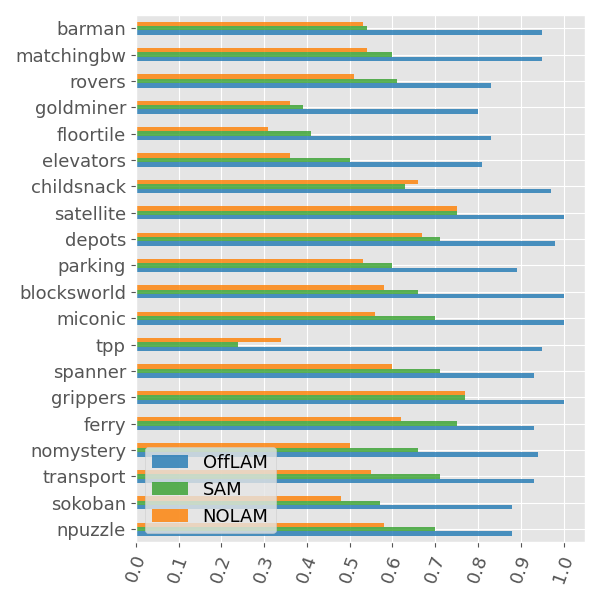
\includegraphics[width=\textwidth]{figures/10_traces_mini/syn_precision.png}
%     \caption{Syntactic precision}
%   \end{subfigure}
%   \\
%   % \begin{subfigure}[b]{0.24\textwidth}
%   %   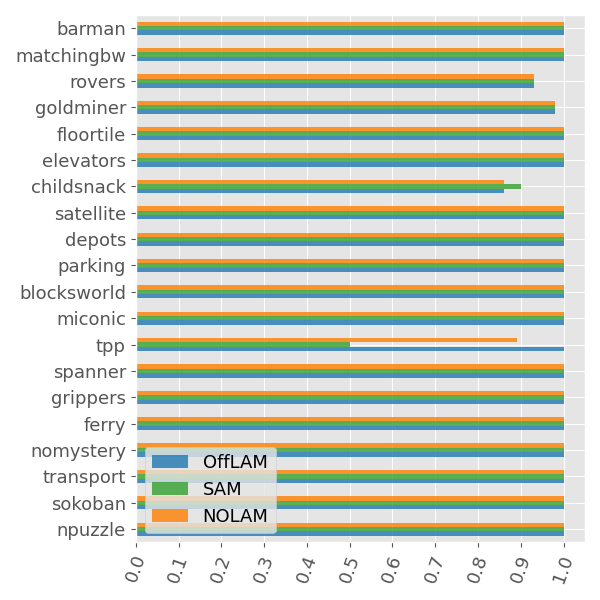
\includegraphics[width=\textwidth]{figures/10_traces_mini/syn_recall.png}
%   %   \caption{Syntactic recall}
%   % \end{subfigure}
%   \begin{subfigure}[b]{0.6\columnwidth}
%     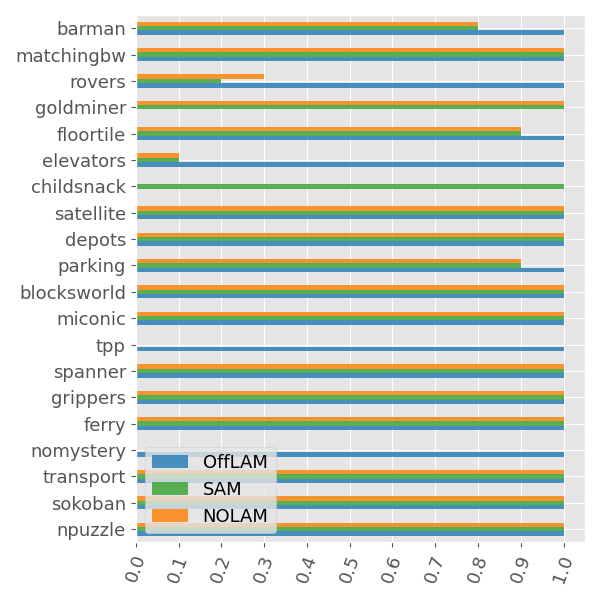
\includegraphics[width=\textwidth]{figures/10_traces_mini/solving.png}
%     \caption{Problem solving ratio}
%   \end{subfigure}
%   \\
%   \begin{subfigure}[b]{0.6\columnwidth}
%     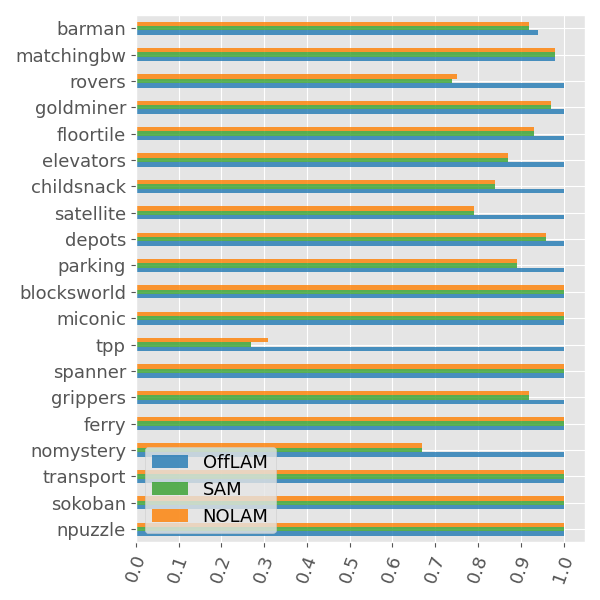
\includegraphics[width=\textwidth]{figures/10_traces_mini/app_recall.png}
%     \caption{Applicability recall}
%   \end{subfigure}




%   \caption{Evaluation metrics when learning from a training set $\Ttrain$ with $10$ traces for every domain.}
%   \label{fig:exp-mini}
% \end{figure} 


% OPTION B

\begin{figure}[ht]
% \label{fix:exp-results}
  \centering

  \begin{subfigure}[b]{\columnwidth}
    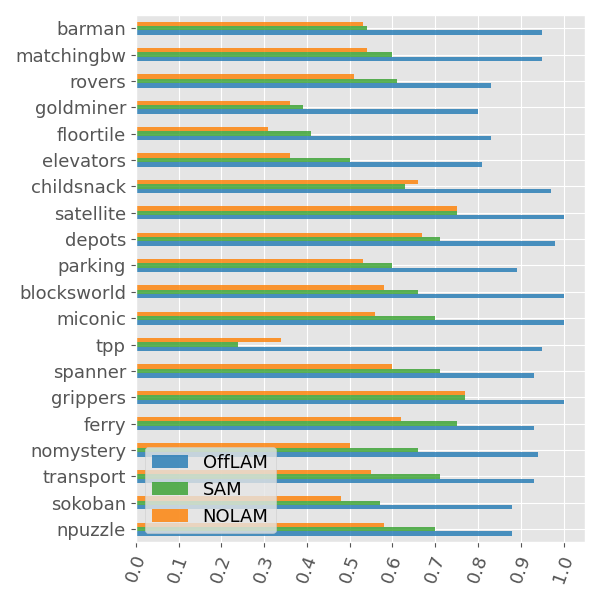
\includegraphics[width=\textwidth]{figures/10_traces_mini/syn_precision.png}
    \caption{Preconditions syntactic precision}
    \label{fig:syn-precision}
  \end{subfigure}
  \hfill
  % \begin{subfigure}[b]{0.24\textwidth}
  %   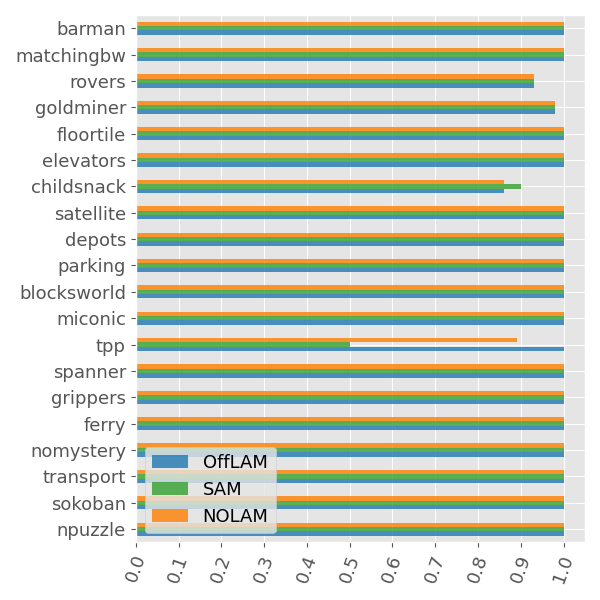
\includegraphics[width=\textwidth]{figures/10_traces_mini/syn_recall.png}
  %   \caption{Syntactic recall}
  % \end{subfigure}
  \begin{subfigure}[b]{\columnwidth}
    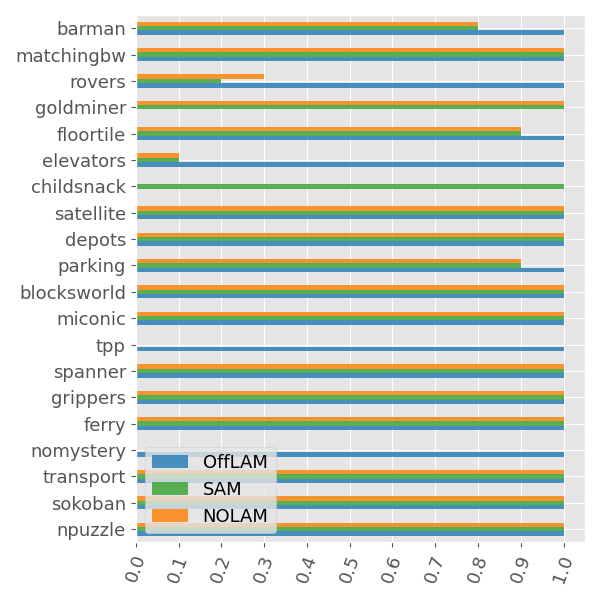
\includegraphics[width=\textwidth]{figures/10_traces_mini/solving.png}
    \caption{Problem solving ratio}
    \label{fig:solving-ratio}
  \end{subfigure}
  \hfill
  \begin{subfigure}[b]{\columnwidth}
    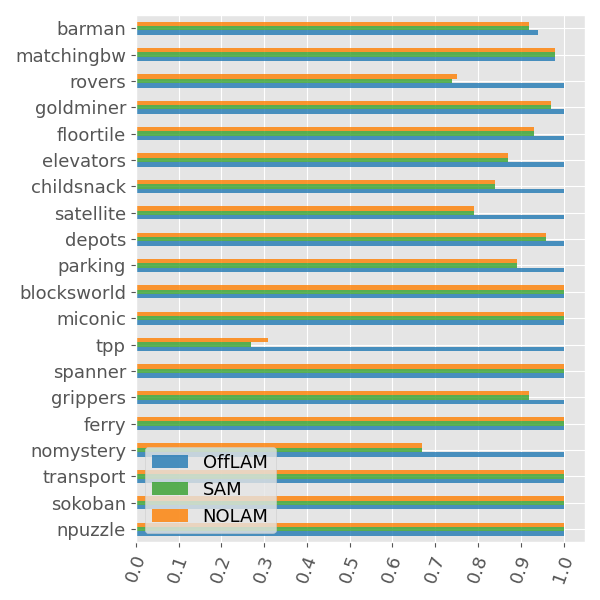
\includegraphics[width=\textwidth]{figures/10_traces_mini/app_recall.png}
    \caption{Applicability recall}
  \end{subfigure}




  \caption{Evaluation metrics for the models learned by \samshort{}, \offlam{} and \nolam{} from a training set $\Ttrain$ of $10$ traces for every domain.}
  \label{fig:exp-mini}
\end{figure} 

% \roni{Writing standard: we show here 3 concrete algorithms, not 3 approaches.}

To demonstrate our evaluation process, we used it to evaluate three state-of-the-art domain model learning algorithms, namely \samshort~\citep{juba2021safe}, \offlam~\citep{LAMANNA2025104256}, and \nolam~\citep{Lamanna24}. The results of our evaluation  are described below. Due to space constraints only a subset of the results are shown in Figure~\ref{fig:exp-mini}. All the experiments were run on a CPU Apple M1 Pro with 16 GB of RAM.
%We evaluated the learning algorithms on standard benchmark domains using the proposed metrics. 





\miniparagraph{Syntactic similarity} 
% We report syntactic precision and recall using the \emph{simple} aggregation across the preconditions and effects of all actions. \roni{It was written here that we use the cumulative aggregation and not the average here. But, this is a syntactic similarity metric, you can only aggregate over actions. Commenting this out}
Both \samshort{} and \nolam{} exhibited relatively low precondition precision ($<0.8$) across all domains, as they assume the presence of negative preconditions and include them in the learned domains. 
In contrast, \offlam{} assumes that domains do not include negative preconditions, which is a correct assumption for our benchmarks, leading to higher precision values.
In terms of precondition recall, \samshort{}'s low values stemmed from its inability to learn some actions entirely, i.e., the actions have all the preconditions and no effects, while \offlam{} and \nolam{} struggled to learn specific predicates due to domain inconsistencies (e.g., in \textsc{rovers}) or the presence of constants not bound to action parameters (e.g., in \textsc{childsnack}).
% \roni{All this discusses preconditions. What about the syntactic similarity of effects?}
% \leo{
In terms of effects, both \offlam{} and \nolam obtained syntactic precision and recall of $1$ in all domains except \textsc{rovers} (because of inconsistent effects), \textsc{goldminer} (because of an unobserved negative effect) and \textsc{childsnack} (for an unobserved positive effect). \samshort{} achieved effects the same results except for \textsc{tpp}, where it only achieved 50\% recall.
% for both positive and negative effects.} do we separate the two types in our evaluation?
% However, the domains used in the experiments do not include negative preconditions. 
% This is due to additional preconditions, as both algorithms include negative preconditions in the learned domains, which are always absent in the reference domains. For instance, in the \textsc{blocksworld} domain, the lifted action \textsc{pick\_up}$(x)$ for a block $x$ has the precondition $\textit{handempty}()$, which implies $\textit{holding}(x)$ is false. 
% % However, the domains learned by \samshort{} and \nolam{} include such negative preconditions, which lowers their syntactic precision. 
% In contrast, \offlam{} assumes domains do not include negative preconditions, resulting in more concise domains and higher precision. However, this metric's sensitivity to such additions is a limitation, as it can penalize the inclusion of predicates that implicitly hold true in the domain. 
% Regarding the aggragated recall \roni{recall of preconditions or effects?} \argaman{The metric is calculated as a combination of the two.}, all algorithms performed similarly, with perfect recall in all but four domains -- \textsc{tpp}, \textsc{childsnack}, \textsc{goldminer} and \textsc{rovers}.
% The lower recall in those domains mainly stem from missing effects.
% A prominent example is \textsc{tpp} domain, with \samshort{} having the lowest recall (i.e., $0.5$). 
% This is due to its assumption that actions cannot be executed with the same object bound to multiple parameters—an assumption that does not hold in this domain.\footnote{This is referred to as the \textit{injective binding assumption} in the \sam learning paper.} 
% The ESAM algorithm remedies this limitation~\citep{juba2021safe}.
% % In \textsc{childsnack} domain, \offlam and \nolam both 
% \roni{This explains why SAM did not work well, but what about the other algorithms? what is unique in these domains. If we do not know, that is also Ok, this is not a paper that is intended to explain the algorithms just show the benchmark}
% \leo{In \textsc{childsnack}, both \offlam{} and \nolam{} misses a positive precondition of action $put\_on\_tray$ involving a constant $kitchen$, since they do not support constants. On the opposite, \samshort{} do support constants. In \textsc{rovers}, all approaches cannot learn some positive and negative effects; indeed the IPC version of \textsc{rover} contains some inconsistent effects. In \textsc{gold-miner}, all approaches do not learn a negative effect because it is never observed in the trajectories.}



\miniparagraph{Predicted applicability} 
By design, \samshort{} and \offlam{} initially assume the preconditions of each lifted action to be the set of all possible preconditions, and remove unnecessary preconditions that are not consistent with the input trajectories, resulting in perfect applicability precision. Notably, \nolam{} achieves perfect applicability precision even without such assumption.
The only outlier is the \textsc{childsnack} domain, where both \nolam{} and \offlam{} have a slight decrease in the precision due to the constant in the domains (which is not supported by these algorithms).
% in the precision due to $put\_on\_tray$'s precondition involving $kitchen$.
% This results from the domain including a constant -- $kitchen$ -- in a predicate of the action $put\_on\_tray$'s preconditions. 
% Indeed, this constant is not part of the action's parameters, which causes it not to be learned.
% \roni{Not clear. Do you mean NOLAM and Offlam do not support constants and SAM does?}\leo{Yes, I added a comment about this in the previous paragraph}
\offlam{} achieved the best performance in terms of applicability recall with perfect recall values in all domains except \textsc{barman}, which had a slight decrease in its recall due to a single literal miss-classified as a precondition. 
% \leo{with only a slight decrease in its recall value due to a false positive precondition for action $empty\_shot$. This results from \offlam{} assuming no negative preconditions, which prevents it from learning unnecessary ones.}
% allows to remove redundant ones with less observations than \samshort{} and \nolam{} that assume the existence of negative preconditions as well. 
Notably, the unnecessary negative preconditions learned by \samshort{} and \nolam{} only significantly impacted the recall for the \textsc{tpp} domain; indeed, all other domains had applicability recall values exceeding $0.6$. 


\miniparagraph{Predicted effects} 
% Across all domains, all algorithms achieved perfect precision and recall. This is attributed to the fact that each action in the trace dataset was observed at least once, ensuring that all effects present in the training trajectories were successfully learned.\roni{Not convincing. Observing once is not enough.}
All algorithms achieved perfect precision and recall across all domains. 
By design, \samshort{} and \offlam{} provides effects syntactic precision equal to $1$ (this also holds for \nolam{} as the trajectories are un-noisy and fully observable), since an action's effect is learned only when a literal becomes true/false after observing such action execution in some trajectory transition. This prevents \samshort{} and \offlam{} from learning unnecessary effects, hence makes the false positives for the predicted effects equal to $0$, and the precision equal to $1$. 
Furthermore, the predicted effects only consider actions applicable according to the learned domain and real environment, and every lifted action execution is observed at least once in the set of trajectories. Therefore, evaluating the actions is only performed when the actions are applicable according to the learned domain. Thus resulting in states that were already observed in the train trajectories.
% Other approaches that are less conservative than our tested algorithms might perform a different approach to learning the effects, resulting in different predictive values. 
Other, less conservative approaches may follow different effect-learning strategies, potentially leading to different precision and recall outcomes.

% when evaluating the predicted effects of an action
% $a$ in a state $s$, there is a trajectory state which satisfies the precondition of $a$ as $s$ does (otherwise $a$ would not be applicable in $s$), and thus if a literal does not change after executing $a$ in such trajectory state, then either the literal is not an effect of $a$ or it is both an effect and a precondition of $a$, which already holds in $s$ (e.g. a positive effect which is already true in $s$). Hence FN equals $0$ and the predicted effects recall equals $1$.
% precision equals 1 because of the effects syntactic precision being equal to 1 and the preconditions being a superset of the real preconditions: no false effects implies no `false changes` in the destination state reached after executing an applicable action. 



\miniparagraph{Problem-solving} 
\offlam{} achieved the highest problem-solving ratio across all domains except for \textsc{childsnack} and \textsc{goldminer}. Notably, in the \textsc{nomystery} and \textsc{tpp} domains, it is the only algorithm to produce a model capable of solving the entire test set.
In the \textsc{elevators} and \textsc{rovers} domains it highly outperforms both \samshort{} and \nolam{} with 85\% and 70\% increase in the 
solving rates respectively.
The difficulty in solving problems for \samshort{} and \nolam{}, is mainly due to the learned domains having unnecessary negative preconditions. 
% Specifically, in these domains, the actions had high arity which resulted in many negative preconditions that were created for them (see Table~\ref{tab:domains} for reference). 
In \textsc{childsnack}, both \offlam{} and \nolam{} produced inapplicable plans due to the missing precondition involving the unsupported constant.
% of $put\_on\_tray$ involving the unsupported constant $kitchen$. 
% This results from the domain having a constant that was not properly learned by these algorithm which was part of the action $put\_on\_tray$'s preconditions.
% An exception is the \textsc{childsnack} domain, which includes a constant unsupported by both NOLAM and OffLAM. 
% \roni{Repetition of the sentence above?}\leo{yes, removed}
% Although plans were generated, they were deemed inapplicable, as shown in Figure~\ref{fig:false-positive-plans}.
Similarly, the plans produced with the models learned by \offlam{} are inapplicable due to a missing negative effect which affects the precondition of subsequent plan actions.
% $(not\; (gold\_at\; ?y))$ of action $fire\_laser$, which affects the precondition of subsequent plan actions.
% We also observed that in the \textsc{goldminer} all of the plans generated using the domains \offlam learned were deemed inapplicable. This resulted from \offlam not learning the effect $(not\; (gold\_at\; ?y))$ which was crucial to the consistency of the resulting plans. 
% Because 
Such effect was never observed in the input trajectories. Interestingly, \sam and \nolam, learned the unobserved negative effect as a negative precondition, which allows to compute valid plans.


\begin{table}[b!]
\resizebox{\columnwidth}{!}{
\addtolength{\tabcolsep}{-0.4em}
\begin{tabular}{l|l|l|l|l|l|l}
% \toprule
\hline
Domain & \multicolumn{2}{c|}{Syntactic} & \multicolumn{2}{c|}{Applicability} & Solv. \% $\uparrow$ & False \% $\downarrow$ \\
 & \makecell[c]{P$\uparrow$} & \makecell[c]{R$\uparrow$} & \makecell[c]{P$\uparrow$} & \makecell[c]{R$\uparrow$} &  & \\
% \midrule
\hline
barman  & 0.95 $^{2}$ & 1.00 $^{1,2,3}$ & 1.00 $^{1,2,3}$ & 0.94 $^{2}$ & 1.00 $^{2}$ & 0.00 $^{1,2,3}$ \\
blocksworld  & 1.00 $^{2}$ & 1.00 $^{1,2,3}$ & 1.00 $^{1,2,3}$ & 1.00 $^{1,2,3}$ & 1.00 $^{1,2,3}$ & 0.00 $^{1,2,3}$ \\
childsnack & 0.97 $^{2}$ & 0.90 $^{1}$ & 1.00 $^{1}$ & 1.00 $^{2}$ & 1.00 $^{1}$ & 0.00 $^{1}$ \\
depots  & 0.98 $^{2}$ & 1.00 $^{1,2,3}$ & 1.00 $^{1,2,3}$ & 1.00 $^{2}$ & 1.00 $^{1,2,3}$ & 0.00 $^{1,2,3}$ \\
elevators  & 0.81 $^{2}$ & 1.00 $^{1,2,3}$ & 1.00 $^{1,2,3}$ & 1.00 $^{2}$ & 1.00 $^{2}$ & 0.00 $^{1,2,3}$ \\
ferry  & 0.93 $^{2}$ & 1.00 $^{1,2,3}$ & 1.00 $^{1,2,3}$ & 1.00 $^{1,2,3}$ & 1.00 $^{1,2,3}$ & 0.00 $^{1,2,3}$ \\
floortile & 0.83 $^{2}$ & 1.00 $^{1,2,3}$ & 1.00 $^{1,2,3}$ & 1.00 $^{2}$ & 1.00 $^{2}$ & 0.00 $^{1,2,3}$ \\
goldminer & 0.8 $^{2}$ & 0.98 $^{1,2,3}$ & 1.00 $^{1,2,3}$ & 1.00 $^{2}$ & 1.00 $^{1,3}$ & 0.00 $^{1,3}$ \\
grippers & 1.00 $^{2}$ & 1.00 $^{1,2,3}$ & 1.00 $^{1,2,3}$ & 1.00 $^{2}$ & 1.00 $^{1,2,3}$ & 0.00 $^{1,2,3}$ \\
matchingbw & 0.95 $^{2}$ & 1.00 $^{1,2,3}$ & 1.00 $^{1,2,3}$ & 0.98 $^{1,2,3}$ & 1.00 $^{1,2,3}$ & 0.00 $^{1,2,3}$ \\
miconic & 1.00 $^{2}$ & 1.00 $^{1,2,3}$ & 1.00 $^{1,2,3}$ & 1.00 $^{1,2,3}$ & 1.00 $^{1,2,3}$ & 0.00 $^{1,2,3}$ \\
nomystery & 0.94 $^{2}$ & 1.00 $^{1,2,3}$ & 1.00 $^{1,2,3}$ & 1.00 $^{2}$ & 1.00 $^{2}$ & 0.00 $^{1,2,3}$ \\
npuzzle & 0.88 $^{2}$ & 1.00 $^{1,2,3}$ & 1.00 $^{1,2,3}$ & 1.00 $^{1,2,3}$ & 1.00 $^{1,2,3}$ & 0.00 $^{1,2,3}$ \\
parking & 0.89 $^{2}$ & 1.00 $^{1,2,3}$ & 1.00 $^{1,2,3}$ & 1.00 $^{2}$ & 1.00 $^{2}$ & 0.00 $^{1,2,3}$ \\
rovers & 0.83 $^{2}$ & 0.93 $^{1,2,3}$ & 1.00 $^{1,2,3}$ & 1.00 $^{2}$ & 1.00 $^{2}$ & 0.00 $^{1,2,3}$ \\
satellite & 1.00 $^{2}$ & 1.00 $^{1,2,3}$ & 1.00 $^{1,2,3}$ & 1.00 $^{2}$ & 1.00 $^{1,2,3}$ & 0.00 $^{1,2,3}$ \\
sokoban & 0.88 $^{2}$ & 1.00 $^{1,2,3}$ & 1.00 $^{1,2,3}$ & 1.00 $^{1,2,3}$ & 1.00 $^{1,2,3}$ & 0.00 $^{1,2,3}$ \\
spanner & 0.93 $^{2}$ & 1.00 $^{1,2,3}$ & 1.00 $^{1,2,3}$ & 1.00 $^{1,2,3}$ & 1.00 $^{1,2,3}$ & 0.00 $^{1,2,3}$ \\
tpp & 0.95 $^{2}$ & 1.00 $^{2}$ & 1.00 $^{1,2,3}$ & 1.00 $^{2}$ & 1.00 $^{2}$ & 0.00 $^{1,2,3}$ \\
transport & 0.93 $^{2}$ & 1.00 $^{1,2,3}$ & 1.00 $^{1,2,3}$ & 1.00 $^{1,2,3}$ & 1.00 $^{1,2,3}$ & 0.00 $^{1,2,3}$ \\
% \bottomrule
\hline
\end{tabular}
}
\caption{Best metric values for every domain obtained among \sam, \offlam, \nolam, respectively denoted by 1,2, and 3; P indicates the precision and R the recall, $\uparrow$ (resp. $\downarrow$) denotes the higher (resp. lower) the better. The predicted effects precision and recall equal $1$ for all approaches in all domains.}
\label{tab:best}
\end{table}




% \hline
% barman  & 0.95 $^{2}$ & 1.00 $^{1,2,3}$ & 1 $^{1,2,3}$ & 0.94 $^{2}$ & 1 $^{2}$ & 0 $^{1,2,3}$ \\
% blocksworld  & 1 $^{2}$ & 1 $^{1,2,3}$ & 1 $^{1,2,3}$ & 1 $^{1,2,3}$ & 1 $^{1,2,3}$ & 0 $^{1,2,3}$ \\
% childsnack & 0.97 $^{2}$ & 0.9 $^{1}$ & 1 $^{1}$ & 1 $^{2}$ & 1 $^{1}$ & 0 $^{1}$ \\
% depots  & 0.98 $^{2}$ & 1 $^{1,2,3}$ & 1 $^{1,2,3}$ & 1 $^{2}$ & 1 $^{1,2,3}$ & 0 $^{1,2,3}$ \\
% elevators  & 0.81 $^{2}$ & 1 $^{1,2,3}$ & 1 $^{1,2,3}$ & 1 $^{2}$ & 1 $^{2}$ & 0 $^{1,2,3}$ \\
% ferry  & 0.93 $^{2}$ & 1 $^{1,2,3}$ & 1 $^{1,2,3}$ & 1 $^{1,2,3}$ & 1 $^{1,2,3}$ & 0 $^{1,2,3}$ \\
% floortile & 0.83 $^{2}$ & 1 $^{1,2,3}$ & 1 $^{1,2,3}$ & 1 $^{2}$ & 1 $^{2}$ & 0 $^{1,2,3}$ \\
% goldminer & 0.8 $^{2}$ & 0.98 $^{1,2,3}$ & 1 $^{1,2,3}$ & 1 $^{2}$ & 1 $^{1,3}$ & 0 $^{1,3}$ \\
% grippers & 1 $^{2}$ & 1 $^{1,2,3}$ & 1 $^{1,2,3}$ & 1 $^{2}$ & 1 $^{1,2,3}$ & 0 $^{1,2,3}$ \\
% matchingbw & 0.95 $^{2}$ & 1 $^{1,2,3}$ & 1 $^{1,2,3}$ & 0.98 $^{1,2,3}$ & 1 $^{1,2,3}$ & 0 $^{1,2,3}$ \\
% miconic & 1 $^{2}$ & 1 $^{1,2,3}$ & 1 $^{1,2,3}$ & 1 $^{1,2,3}$ & 1 $^{1,2,3}$ & 0 $^{1,2,3}$ \\
% nomystery & 0.94 $^{2}$ & 1 $^{1,2,3}$ & 1 $^{1,2,3}$ & 1 $^{2}$ & 1 $^{2}$ & 0 $^{1,2,3}$ \\
% npuzzle & 0.88 $^{2}$ & 1 $^{1,2,3}$ & 1 $^{1,2,3}$ & 1 $^{1,2,3}$ & 1 $^{1,2,3}$ & 0 $^{1,2,3}$ \\
% parking & 0.89 $^{2}$ & 1 $^{1,2,3}$ & 1 $^{1,2,3}$ & 1 $^{2}$ & 1 $^{2}$ & 0 $^{1,2,3}$ \\
% rovers & 0.83 $^{2}$ & 0.93 $^{1,2,3}$ & 1 $^{1,2,3}$ & 1 $^{2}$ & 1 $^{2}$ & 0 $^{1,2,3}$ \\
% satellite & 1 $^{2}$ & 1 $^{1,2,3}$ & 1 $^{1,2,3}$ & 1 $^{2}$ & 1 $^{1,2,3}$ & 0 $^{1,2,3}$ \\
% sokoban & 0.88 $^{2}$ & 1 $^{1,2,3}$ & 1 $^{1,2,3}$ & 1 $^{1,2,3}$ & 1 $^{1,2,3}$ & 0 $^{1,2,3}$ \\
% spanner & 0.93 $^{2}$ & 1 $^{1,2,3}$ & 1 $^{1,2,3}$ & 1 $^{1,2,3}$ & 1 $^{1,2,3}$ & 0 $^{1,2,3}$ \\
% tpp & 0.95 $^{2}$ & 1 $^{2}$ & 1 $^{1,2,3}$ & 1 $^{2}$ & 1 $^{2}$ & 0 $^{1,2,3}$ \\
% transport & 0.93 $^{2}$ & 1 $^{1,2,3}$ & 1 $^{1,2,3}$ & 1 $^{1,2,3}$ & 1 $^{1,2,3}$ & 0 $^{1,2,3}$ \\
% % \bottomrule
% \hline

% \roni{Important: Can we add to the domains table the columns: Constants (Const.), Injective binding (Inj. Bind), and Negative preconditions (Neg. Pre.)? this will connect to the reults we observed.}
% \leo{added. I am not sure about the injective binding assumption since even though an action can take as input objects of the same type, then the fact that it (can) actually involves the same object multiple times depends on the domain and traces. I am not sure this is easily deducible from the action signature only, as I currently did}


% \roni{The results are Ok. Perhaps would be good to add a summary paragraph that says something like As the results show, different algorithms work well in different domains and for different metrics. }
% \leo{I wrote a draft for this }

% \leo{
\miniparagraph{Results summary} 
Table \ref{tab:best} lists the best performance for each metric and domain on the proposed benchmark. The superscripts in each cell indicate which of the evaluated algorithms --- \sam{}, \offlam{}, and \nolam{} --- obtained the best performance in this metric and domain. As the results show, while the algorithms are able to reach impressive performance in our benchmark, one can see that different algorithms perform better in different domains and for different metrics. 
For example, \offlam{} provides better syntactic precondition precision than \samshort{} and \nolam{} in all domains. However, it fails to solve some test problems in \textsc{goldminer} since it does not learn negative effects (while \sam and \offlam{} can learn them). 
% are not learned, as in \textsc{goldminer} domain; while this is not the case for \samshort{} and \nolam{}. 
Indeed, the syntactic precision performance gap between \offlam{} and other approaches (Figure \ref{fig:syn-precision}) is not reflected in terms of problem-solving (Figure \ref{fig:solving-ratio}) as, e.g., in domain \textsc{matchingbw}. 
This provides empirical evidence of the drawbacks in syntactic similarity discussed in Section \ref{sec:problem-setting}.
Interestingly, the different approaches to deal with action objects binding can significantly impact the performance in domains where the injective action binding assumption is violated, as in \textsc{elevators} and \textsc{tpp}.  


% BACKUP IF I DO DAMAGE
% We assessed the best performance of three state-of-the-art approaches on the proposed benchmark (Table \ref{tab:best}). As the results show, different algorithms perform better in different domains and for different metrics. On the one hand, \offlam{} provides better syntactic precision than \samshort{} and \nolam{}, on the other hand, it assumes there are no negative preconditions, which can degrade problem-solvability performance when some negative effects are not learned, as in \textsc{goldminer} domain; while this is not the case for \samshort{} and \nolam{}. 
% Moreover, the syntactic precision performance gap between \offlam{} and other approaches (Figure \ref{fig:syn-precision}) is not reflected in terms of problem-solving (Figure \ref{fig:solving-ratio}) as, e.g., in domain \textsc{matchingbw}. This provides empirical evidence of the drawbacks in syntactic similarity discussed in Section \ref{sec:problem-setting}.
% Interestingly, the different approaches to deal with action objects binding can significantly impact the performance in domains where the injective action binding assumption is violated, as in \textsc{elevators} and \textsc{tpp}.  


\section{Bridging Representation Gaps}
\label{sec:bridging-gap}
% \roni{Moved this section to after the results, as currently the results do not have any aspect of this so it looks wierd.}
% Motivation: representation may be different learning
So far, we assumed the input trajectories and the learned domain model use the same representation (Assumption A2). Next, we relax this assumption and propose a paradigm for comparing domain model learning algorithms across different representations. 
We limit the discussion to the case where input representation and the learned domain still follow a classical planning representation, as opposed to an image-based or other, more-involved types of representations. 
Nevertheless, existing domain model learning algorithms may output domain models that use a different representation than the input representation.
% \leo{It was not immediately clear to me that `existing domain model learning algorithms` refer to classical planning domains learning algorithms , the second sentence seems to me more general, maybe it can be swapped with the previous one, for example: indeed, existing domain model learning algorithms may output domain models that use a different representation than the input representation [add cit?]. We limit the discussion to the case where the learned domain is still a classical planning domain, as opposed to an images-based or other more involved types of representations. }

% Concrete examples
In some cases, these representation differences are minimal, e.g., using a different ordering of the parameters or object types~\cite{xi2024neuro}. % \leo{can we add a cit?}. \roni{this is not a perfect cite. If we have a better one that would be good.}
In other cases, the differences are more significant. 
For example, the ESAM algorithm~\citep{juba2021safe} outputs a domain model with additional \emph{proxy actions}. 
These proxy actions do not exist in the environment and are used to resolve ambiguities in the mapping of objects to parameters.
In a related manner, \cite{Hankui2013RefiningModels} also create additional macro actions alongside refining the model to turn the input sequences into solutions. 
% \roni{@Pascal: you mentioned a related paper that learned macro actions. Can you add here a citation about it and maybe a sentence on how it relates?}\pascalSr{done, kind-of -- I don't think the authors did a good job explaining what their macro actions are actually required for; I found that weird... So, I can't say much about the relation.}
% \roni{I think it's good enough -TNX!}
% \yarin{added LOCM:}
Similarly, the LOCM algorithm~\citep{cresswell2013acquiring} creates a state representation that is significantly different from the input representation, based on the states of finite-state machines it creates from the given action sequences in the trajectory. 
%-with no access to intermediate state information or predicate names-and outputs action schemas using \emph{proxy predicates}. 
% induces finite-state machines solely from action sequences-with no access to intermediate state information or predicate names-and outputs action schemas using \emph{proxy predicates}. 
% (e.g., \texttt{object\_state0}, \texttt{object\_state1(agent)}). 
% These proxy predicates are not part of the original domain but are introduced as a mechanism to infer the semantics of the original predicates. 
% For example, a learned transition from \texttt{object\_state1} to \texttt{object\_state0} may represent an object being put down, corresponding to a change in the original predicate \texttt{holding(agent, object)}.
\roni{@All: More examples?}
\mauro{OpMaker2 generates classical planning models in OCL language \cite{mccluskey2010action}}
\roni{@Mauro: I read briefly the OpMaker2 and didn't fully understand. Can you write a sentence or two on this. It was not clear to me if OpMaker2 outputs a PDDL or something else.}
\leo{I did not understand what are the assumptions about the input trajectories representation, if any. For example, do we consider visual trajectories? If yes, what about adding latplan? it uses visual trajectories and learns a classical planning model}\roni{For now I clarified above that we focus on symbolic input representation, so we can discuss this in the next subsection.}

% Using each of the previously proposed metrics in such cases, where the input representation is different from the learned domain model representation, is different. 



\subsection{The Encoder-Decoder Mechanism}
Let $R_E$ denote the input representation and let $R_M$ denote the representation of the learned domain model. 
% The input trajectories are given in $R_E$, while the output of a planner that uses the learned domain model is in $R_M$. 
% To allow the comparison of the learned domain model with the reference domain model, we need 
To bridge the gap between these two representations, we require every domain model learning algorithm to output 
a \emph{representation encoder} and a \emph{representation decoder} in addition to the learned model. 
% We describe these two components below.  
The \emph{encoder} transforms states and actions in $R_E$ to corresponding states and actions in the learned domain representation $R_M$. 
The \emph{decoder} performs the reverse transformation, mapping states and actions in $R_M$ to corresponding states and actions in $R_E$.


Formally, let $A_E$ and $A_M$ be the set of actions in the environment and in the learned domain models, respectively, and let $S_E$ and $S_M$ be the set of states in the real and learned domain models, respectively. The power set is denoted by $P(X)$, which is the set of all subsets of $X$. 
The encoder is required to implement the following set of functions:
\begin{itemize}
    \item $\encodea: S_E\times A_E\rightarrow P(A_M)$, returns the actions in $A_M$ representing the application of $a\in A_E$ in a given state $s \in S$.\footnote{This definition implicitly assumes a single action in the learned domain is mapped to a single action in the environment. This assumption is reasonable, but one may produce an domain model in which a sequence of actions corresponds to a single action in the environment. For such cases, the above definition should be revised such that encoding an action return a set of sequences of actions. We avoid this for simplicity.}
    % \roni{Incorporating a great comment by Christian. Is it clear?} \cm{Yep, reads good to me!}} tnx!
    \item ${\encodes: S_E\rightarrow S_M}$, returns the state in $S_M$ that represents the state $s\in S_E$. 
    % \yarin{returns the state $s \in S$ as its representation in $S_M$}
\end{itemize}
The decoder must implement the following functions:
\begin{itemize}
    \item ${\decodea: A_M\rightarrow A_E}$, returns the action in $E$ corresponding to the action in $M$. 
    % \yarin{returns the action $a \in A_M$ as its representation in $A$}roni: not sure: what is "as its representation" part?}
    \item ${\decodes: S_M\rightarrow S_E}$, returns the state in the input representation that represents a given state in $S_M$. 
    % \yarin{returns the state $s \in S_M$ as its representation in $S$}\roni{I do not understand. Let's talk about this.}
\end{itemize}
Next, we describe how to use these encoder/decoder methods to compute the predictive power and problem-solving metrics across even when the input representation is different from the one returned by the evaluated domain model learning algorithm.




% \end{itemize}
    
%     are a proxy of the action $a$.
    
%     $\text{ and} \\ encodeAction(s,a,m^*,m)$=
% ${\{a'\in m| a'\ is\ a\ proxy\ action\ of\ a\}}$
%     \item ${\mathit{decodeAction}: A_{m}\rightarrow  A_{m^*} }$ $\text{ and } {\mathit{decodeAction}(s,a',m^*,m)}$$  a^*\in A_{m^*}$ s.t. $a^*$ is a proxy of $a$. 



% \begin{itemize}
%     \item $encodePlan: \{\pi_{m^*}\in \pi(A_{m^*})\}\rightarrow P(\pi_{m}\in \pi(A_{m}))$
%     \item $\mathit{decodePlan}:\{\pi_{m}\in \pi(A_{m})\} \rightarrow  \{\pi_{m^*}\in \pi(A_{m^*})\}$
% \end{itemize}

% \begin{itemize}
%     \item $encodePredicates:P( P_{m^*}) \rightarrow  P(P_m) \\$  and $encode{Predicates}(P'\subseteq P^*,m^*,m) = P''\subseteq P_m$
%     \item $\mathit{decodePredicates}: P( P_{m}) \rightarrow  P(P_{m^*}) $  and $\mathit{decodePredicates}(P'\subseteq P_{m^*},m^*,m) = P''\subseteq P_m$. 
% \end{itemize}

\miniparagraph{Predictive power metrics}
To adapt the predicted applicability metric, we only modify the way $\app_M(a,\stest)$ is computed to consider different state encodings and the possibility that multiple actions in $M$ may decode to $a$. 
Formally, let $\app_M(a,s)$ be true if $a$ is applicable in $s$ according to $M$. Then $\app_M(a,\stest)$ is redefined as follows:
\begin{equation}
    \large\{s \mid s\in\stest  \wedge 
        \exists a': \decodea(a')=a  
        \wedge \app_M(a',\encodes(s))\large\}        
\end{equation}
That is, we consider an action $a\in A$ to be applicable in a state $s\in\stest$ according to the learned model $M$ if there exists an action $a'\in A_M$ that is decoded to $a$ and is applicable in $\encodes(s)$ according to $M$. 
The predicted effects metrics are adapted 
by replacing $a_M(s)$ with $a^E_M(s)$, which is defined as follows. 
First, we find an action $a'\in A_m$ that satisfies $\decodea(a')=a$ and 
$\app_M(a',\encodes(s))$.\footnote{If none such exists, we cannot compare predicted effects. If more than one such action exists, we choose arbitrarily one of them.} 
Then, we compute $a^E_m(s)=a'_M(\encodes(s))$

\roni{Would be great if someone would add an example of this.}

\miniparagraph{Problem-solving metrics} 
Adapting the problem-solving metrics to use the encoder-decoder mechanism is straightforward. 
For every problem in \ptest we encode the initial state, obtaining a set of problems that can be given to a planner with the learned domain model ($M$). 
Then, the planner is run on each of these problems to attempt to solve them.
In cases where a plan was returned by the planner, we then validate its correctness by decoding the actions in the returned plan and trying to run it in the environment. 

% the encoded problem with the learned model. 

% and apply a planner with the learned domain model to attempt to generate a plan. 
% To validate this plan, we use the \decodea function on all the actions in the plan 
% and simulate them in the environment. 


% Finally, the decoder uses \decodea to decode the solution plan from the learned model representation to the input representation. 
% This allows checking if a plan has been found and if it is valid according to the reference domain model. 


\subsection{Examples of Encoder-Decoder Methods}
Next, we show how to implement the encoder-decoder mechanism several domain model learning algorithms. 
% that use representations different from the input representation. 

\miniparagraph{ESAM~\citep{juba2021safe}}
This algorithm may add proxy actions to the learned domain. 
Each of these proxy actions is mapped to a single action in the input representation. 
Thus, for ESAM the \encodea, \encodes, \decodes functions are the identity functions, but the \decodea function maps a proxy action to its action in the environment. 

\miniparagraph{OBSERVER~\citep{wang1996learning}}
This algorithm deals with grounded domain representations. 
Thus, we require an encoder to move from lifted to grounded representations and then a decoder to map back to a lifted representation.

\miniparagraph{LOCM~\citep{cresswell2013acquiring}} 
The states in the learned domain model are based on the hidden FSM states induced from the traces and while the actions are reuse the original names. Thus, \encodea and \decodea are identity functions, \encodes maps a concrete state $s$ to the unique abstract state $s_M$ whose conjunction of LOCM fluents (each FSM-state predicate with its parameter bindings) matches $s$, and \decodes reconstructs the concrete state by inverting the fluent encoding, assigning each object the attributes implied by its FSM-state predicates.


% . 
% Encoding and decoding states is needed as the states in LOCM model are, as noted above, related to the finite state machine they construct. 

% \cm{Not sure there's enough detail here on LOCM to make it worth it for inclusion.}
% \yarin{maybe something like this: LOCM~\citep{cresswell2013acquiring} produces it's state space from the hidden FSM states induced from the traces and while the actions are reuse the original names. Thus, \encodea and \decodea are identity functions, \encodes maps a concrete state $s$ to the unique abstract state $s_M$ whose conjunction of LOCM fluents (each FSM-state predicate with its parameter bindings) matches $s$, and \decodes reconstructs the concrete state by inverting the fluent encoding, assigning each object the attributes implied by its FSM-state predicates.}
% Decoding is relatively 
% How to encode which is:\yarin{I will complete this}
% Encoder: identity for both state and actions
% % action name and proxy for state predicates
% Decoder: translate proxy predicates to original predicates

% ROSAME-I~\citep{xi2024neuro}: \roni{Maybe Yarin or Argaman can help with this one}
% Encoder: encode to a numeric vector of ones and zeros
% Decoder: map action parameters

% OBSERVER\citep{wang1996learning}: \roni{Anyone can help here?}
% Encoder: from binding to grounded
% Decoder: from grounded predicates and actions to the binding they represent





% : \roni{Either me or someone from my group will write this one}
% Encoder: identity for both state and actions     
% Decoder: translate proxy actions to original actions


% . \yarin{Some action model learning algorithms operate directly in the original input representation $R_{\realm}$, without transforming the state or action spaces. For these algorithms, the learned model uses the same symbols and structure as the input data. As such, there is no need for additional encoding or decoding: the identity function suffices for both.}

% SAM~\citep{juba2021safe}\yarin{or is ut juba2021safe ?}: \roni{Either me or someone from my group will write this one}
% Encoder: identity
% Decoder: identity

% NOLAM~\citep{Lamanna24}:
% Encoder: \leo{identity}
% Decoder: \leo{identity}

% OFFLAM\citep{lamanna2021online}:
% Encoder: \leo{identity}
% Decoder: \leo{identity}

% FAMA~\citep{aineto2019learning}:
% Encoder: identity
% Decoder: identity - maybe change to parameter names?

% ESAM~\citep{juba2021safe}: \roni{Either me or someone from my group will write this one}
% Encoder: identity for both state and actions     
% Decoder: translate proxy actions to original actions

% ROSAME-I~\citep{xi2024neuro}: \roni{Maybe Yarin or Argaman can help with this one}
% Encoder: encode to a numeric vector of ones and zeros
% Decoder: map action parameters

% OBSERVER\citep{wang1996learning}: \roni{Anyone can help here?}
% Encoder: from binding to grounded
% Decoder: from grounded predicates and actions to the binding they represent

% LOCM~\citep{cresswell2013acquiring}:\yarin{I will complete this}
% Encoder: identity for both state and actions
% % action name and proxy for state predicates
% Decoder: translate proxy predicates to original predicates

% \roni{Most important: anyone can help here?}

\subsection{Non-Classical Domain Model Learning}
% \roni{For all: please read and let me know what you think by adding comments in the text (e.g., add text like this ``[[YourName: bla bla bla'']]) or editting.}
% Different input representations
The proposed encoder-decoder evaluation paradigm is designed to be flexible and extensible. 
We list several such directions and outline how our evaluation paradigm can be modified to support them. 

\miniparagraph{Non-symbolic input representation}
Some domain model learning algorithms are designed to learn  from trajectories in which the states are images or given in some other non-symbolic representation, which may be images~\citep{asai2020learning,asai2022classical,xi2024neuro} or even natural language description of the domain~\citep{lindsay2017framer,liu2023llm+, guan2023leveraging}.%\roni{Maybe some recent LLM-based approach?}\yarin{I added LLM+P and LLM+PDDL} GREAT!
Using a domain simulator, an encoder for the initial state, and a decoder for the resulting plans' actions, one can still compute all problem solving and predicted applicability metrics. 
Computing predicted effects would also require a decoder to translate a PDDL state to an image, which may be more challenging to implement. 
% Similar\yarin{the word left in by mistake?}TNX


\miniparagraph{Learning non-classical planning domain models}
Some domain model learning algorithms accept symbolic trajectories as input but still output non-classical domain models. For example, PI-SAM~\citep{le2024learning} outputs a conformant planning domain model and ROSAME~\citep{xi2024neuro} outputs a Probabilistic PDDL model. \roni{I vaguely remember some other work that does this, maybe}
Adapting the predictive power metrics to such cases may not be trivial, but the problem-solving metrics can be adapted in a straightforward manner. 


% Beyond discrete
Some prior work also considered learning domain models that include mixed discrete and continuous state variables~\citep{segura2021discovering,mordoch2023learning}. 
Adapting our evaluation paradigm to such setups is also possible. 
The predicted applicability metrics can be computed as-is, considering both numeric and discrete preconditions.
Problem-solving metrics are easily adaptable, but will require a tolerance of some sort to account for numeric precision issues. 
More involved is the predicted effects metric, which may require defining some loss function for the numeric effects, as learning exactly the same numeric effects as in the reference domain model is unrealistically challenging. 


% Note that in all of these variants and generalizations, the encoder-decoder mechanism allows seamless use of the problem-solving metrics. 





% % Beyond input
% In particular, it can be extended to support input trajectories that are given in representations that are different from classical planning, such as images or other types of data. 
% Another possible extension is to allow the action model learning algorithm to output a domain model that uses a more general type of planning. 
% For example, the action model learning algorithm may output a domain model that uses a probabilistic~\citep{xi2024neuro} or partially observable representation~\citep{le2024learning}. 




% \yarin{We can add a section on trajectories with not successful actions too @Argaman}
% \argaman{I think the paper is already too packed to add this to the discussion...}
% % Online metrics 
% \todo{Maybe talk about metrics for online learning}




%\subsection{Relation to Model Reconciliation}
%\roni{Pascal and Mauro: maybe put here is a discussion on what is model reconciliation and how it relates to our work, and existing model reconciliation metrics?}


%\roni{Pascal and Mauro: same for model repair?}

% \subsection{Trade-Offs and Limitations}
% \brendan{There is a lot of discussion earlier about the motivation for the metrics, but we should recap and include some other bits that did not make it in earlier in this section. I added the above subsection header, and I propose as a start something like the following:\\
% We have proposed two families of metrics with complementary strengths and weaknesses, state-based and problem-based. The state-based metrics are easy to compute and thus provide a clear, well-defined benchmark for estimating the predictive power of methods. This is in contrast to the problem-based metrics that rely on the use of planners that are compute-intensive and, depending on the resources available, may have rather different success rates for the same model representation. The downside of state-based metrics is that in contrast to classical machine learning settings, the ``data distribution'' in planning is highly \emph{non-stationary} (not ``i.i.d.''):  Although the states in the benchmarks were selected to be representative of those visited on trajectories collected using the reference model, this may change. Indeed, the states encountered on a trajectory generated by a planner using a given learned domain-model representation depend on the model. Planners can exploit deficiencies in the learned representation to systematically visit states that are erroneously modeled, if those errors make goals easier to achieve. Thus, the state-based metrics may sometimes be a poor proxy for the utility of the learned model for planning, and here, the problem-based metrics are crucial.}
% \roni{This is super. I'll incorporate it in.}

\section{Discussion}
We explored three family of metrics: syntactic similarity, predictive power, and problem-solving ability. 
There is an interesting trade-off between these families of metrics. 
The syntactic similarity are the easiest to compute, as it only requires comparing the learned domain with a reference domain. However, they are arguably the least useful, and computing them requires many assumptions (Assumptions A1 and A2 above). 
The predictive power metrics characterize well a desirable property of a domain model, and are still relatively easy to compute. 
The downside of these metrics is that in contrast to classical machine learning settings, the ``data distribution'' in planning is highly \emph{non-stationary} (not ``i.i.d.''):  Although the states in the benchmarks were selected to be representative of those visited on trajectories collected using the reference model, this may change. Indeed, the states encountered on a trajectory generated by a planner using a given learned domain-model representation depend on the model. Planners can exploit deficiencies in the learned representation to systematically visit states that are erroneously modeled, if those errors make goals easier to achieve. Thus, the predictive power metrics can be a poor proxy for the utility of the learned model for planning. The problem-based metrics fill in this gap, but, of course, they are the hardest to compute as they require running a planner to compute them. 



% providing a clear, well-defined benchmark for estimating the predictive power of method


% and are still 
% easy to compute and thus provide a clear, well-defined benchmark for estimating the predictive power of methods. This is in contrast to the problem-based metrics that rely on the use of planners that are compute-intensive and, depending on the resources available, may have rather different success rates for the same model representation. The downside of state-based metrics is that in contrast to classical machine learning settings, the ``data distribution'' in planning is highly \emph{non-stationary} (not ``i.i.d.''):  Although the states in the benchmarks were selected to be representative of those visited on trajectories collected using the reference model, this may change. Indeed, the states encountered on a trajectory generated by a planner using a given learned domain-model representation depend on the model. Planners can exploit deficiencies in the learned representation to systematically visit states that are erroneously modeled, if those errors make goals easier to achieve. Thus, the state-based metrics may sometimes be a poor proxy for the utility of the learned model for planning, and here, the problem-based metrics are crucial.}
% \roni{This is super. I'll incorporate it in.}




\section{Conclusion and Future Work}
We proposed a comprehensive evaluation process and a suite of metrics for assessing domain model learning algorithms. Our framework includes three complementary families of metrics: syntactic similarity, predictive power, and problem-solving ability. We analyzed the strengths and limitations of each metric family and how they jointly capture different aspects of model quality.
We also describe our implementation of an evaluation process that computes these metrics, along with a benchmark of domain model learning problems that builds on domains from International Planning Competition (IPC) learning track.
Empirical evaluation of three state-of-the-art domain model learning algorithms on this benchmark reveals that each algorithm exhibits distinct strengths and weaknesses.
To address the challenge of comparing learned domain models expressed in different representations, we further proposed an encoder-decoder mechanism that enables meaningful comparison and metrics across heterogeneous outputs.
The proposed benchmark and evaluation framework are publicly available, providing a foundation for systematic and reproducible research in this area.
Future work may extend the benchmark to include domains beyond the IPC and adapt the evaluation metrics to settings involving online or incremental learning~\citep{lamanna2021online, sreedharan2023optimistic, benyamin2025integratingreinforcementlearningaction, ng2019incremental, chitnis2021glib, jin2022creativity, verma2023autonomous, karia2023epistemic}. 


\commentout{
\miniparagraph{Online learning of domain models}
Here, the learning algorithm is required to learn a domain model by actively interacting with the environment~\citep{lamanna2021online, sreedharan2023optimistic, benyamin2025integratingreinforcementlearningaction, ng2019incremental, chitnis2021glib, jin2022creativity, verma2023autonomous, karia2023epistemic}. 
All the proposed metrics can be computed as-is, after a predefined number of iterations, for the online learning setting. 
However, an additional perspective that may be of interest in online learning of domain models are \emph{cumulative} metrics of the learning process, such as the number of actions performed for learning or the number of problems failed to solve while collecting observations.
% \brendan{Changed terminology. This has little to do with ``regret,'' which refers to fixing, e.g., a single best policy from a class in hindsight as a baseline for comparison.}  Sounds good.
Specific metrics and evaluation for online learning of domain models, however, is beyond the scope of this work. 
}



% we proposed an evaluation process and metrics for domain model learning algorithms. 
% This includes three families of metrics, syntactic similarity, predictive power, and problem-solving ability, and discussed their complementary strengths and weaknesses. 
% % of these metrics and propose an evaluation process for computing them. 
% Then, we described our implementation of this evaluation process and a set benchmark problems based on domains from the IPC. 
% Empirical results on three state of the art domain model learning algorithms over this benchmark show that each algorithm has its pros and cons. 
% Finally, we proposed an encoder-decoder mechanism for comparing domain model learning algorithms that output domains that use different representation. 
% The benchmark and evaluation process we proposed are publicly available, facilitating future research in the field to progress. Future work can also add to our benchmark domains beyond the IPC, as well as extend our metrics to the online learning setting. 


% \section{Conclusion Future Work}
% \roni{I'll fix this text later}
% % TODO VERIFY TEXT BELOW
% We presented a new paradigm for evaluating action 
% model learning algorithms across different representations. In this paradigm, each domain model learning algorithm is required to output a domain model and an encoder-decoder pair. The encoder-decoder pair is used to bridge representation gaps and enable measuring the problem-solving capabilities of the learned domain models. We proposed an evaluation scheme that leverages the encoder-decoder pair to systematically compare learned domain models and described several evaluation metrics. A benchmark suite was also provided to facilitate the evaluation of domain model learning algorithms, based on existing domain models from the International Planning Competition (IPC). We demonstrated our evaluation paradigm by applying it to several domain model learning algorithms, including \sam, ESAM, FAMA, and ROSAME.

% Finally, domain models can also be compared not only in terms of their characteristics, but also in terms of the processes used to learn or generate them \citep{vallati2021quality}, a perspective that is commonly used for assessing conceptual models. This is also a direction for future work. 




\bibliographystyle{kr}
\bibliography{library} 

\supplementary{
\clearpage
\onecolumn
% \leo{there is a command in the preamble to hide supplementary material}
\section*{Supplementary Material: Submission \#316}
%
% \subsection{IPC Domains Statistics} roni: moved to the main tex
% \begin{table*}[ht]
\centering
\resizebox{0.8\columnwidth}{!}{
\addtolength{\tabcolsep}{-0.2em}
    \centering
    \begin{tabular}{l|c|c|c|c|c|c|c|c|c|c}
    % \toprule
    \hline
    Domain & Operators & Predicates & Types & Const. & \multicolumn{2}{c|}{Operators arity} & \multicolumn{2}{c|}{Predicates arity} & Neg. pre. & Inj. ass.\\ 
     &  &  & & & $min$ & $max$ & $min$ & $max$ & & \\ \hline
    % \midrule
barman & 12 & 15 & 9 & no & 2 & 6 & 1 & 2 & no & no \\
blocksworld & 4 & 5 & 1 & no & 1 & 2 & 0 & 2 & no & no \\
childsnack & 6 & 13 & 6 & yes & 2 & 4 & 1 & 2 & no & no \\
depots & 5 & 6 & 9 & no & 3 & 4 & 1 & 2 & no & no \\
elevators & 6 & 8 & 5 & no & 3 & 5 & 2 & 2 & no & no \\
ferry & 3 & 5 & 2 & no & 2 & 2 & 0 & 2 & no & no \\
floortile & 7 & 10 & 3 & no & 3 & 4 & 1 & 2 & no & no \\
goldminer & 7 & 12 & 1 & no & 1 & 2 & 0 & 2 & no & no \\
grippers & 3 & 4 & 4 & no & 3 & 4 & 2 & 3 & no & no \\
matchingbw & 10 & 10 & 2 & no & 2 & 3 & 1 & 2 & no & no \\
miconic & 4 & 6 & 2 & no & 2 & 2 & 1 & 2 & no & no \\
nomystery & 3 & 6 & 5 & no & 3 & 6 & 2 & 3 & no & no \\
npuzzle & 1 & 3 & 2 & no & 3 & 3 & 1 & 2 & no & no \\
parking & 4 & 5 & 2 & no & 3 & 3 & 1 & 2 & no & no \\
rovers & 9 & 25 & 7 & no & 2 & 6 & 1 & 3 & no & no \\
satellite & 5 & 8 & 4 & no & 2 & 4 & 1 & 2 & no & no \\
sokoban & 2 & 4 & 3 & no & 3 & 5 & 1 & 3 & no & no \\
spanner & 3 & 6 & 5 & no & 3 & 4 & 1 & 2 & no & no \\
tpp & 4 & 7 & 7 & no & 3 & 7 & 2 & 3 & no & no \\
transport & 3 & 5 & 6 & no & 3 & 5 & 2 & 2 & no & no \\

    % \hline
    \end{tabular}
    }
    \caption{Details about the domains available in the proposed benchmark.}
    \label{tab:domains}
\end{table*}
%
\vspace{0.8cm}
\subsection{Training Set $\Ttrain$ Statistics}
\begin{table}[ht]
\centering
\resizebox{.45\columnwidth}{!}{
\begin{tabular}{l|c|c|c}
% \toprule
\hline
 Domain & \# States & \# Objects & \# Lifted Actions \\
% \midrule
\hline
barman & 35.80 & 25.10 & 34.80 \\
blocksworld & 23.00 & 7.50 & 22.00 \\
childsnack & 25.50 & 28.40 & 24.50 \\
depots & 21.60 & 28.30 & 20.60 \\
elevators & 25.80 & 14.50 & 24.80 \\
ferry & 27.60 & 14.70 & 26.60 \\
floortile & 35.90 & 53.70 & 34.90 \\
goldminer & 30.00 & 21.00 & 29.00 \\
grippers & 15.50 & 17.60 & 14.50 \\
matchingbw & 25.00 & 9.50 & 24.00 \\
miconic & 21.00 & 10.80 & 20.00 \\
nomystery & 19.80 & 16.80 & 18.80 \\
npuzzle & 30.00 & 29.80 & 29.00 \\
parking & 21.00 & 12.10 & 20.00 \\
rovers & 30.00 & 25.10 & 29.00 \\
satellite & 24.50 & 25.10 & 23.50 \\
sokoban & 26.40 & 60.80 & 25.40 \\
spanner & 20.30 & 21.30 & 19.30 \\
tpp & 30.00 & 17.30 & 29.00 \\
transport & 28.20 & 29.60 & 27.20 \\
% \bottomrule
\end{tabular}
}
\caption{Average number of states, objects, and lifted actions among the set of $10$ trajectories for every domain.}
\label{tab:traj-stats}
\end{table}
\vspace{1cm}

\begin{figure}[ht]
% \label{fix:exp-results}
  \centering

  \begin{subfigure}[b]{0.48\textwidth}
    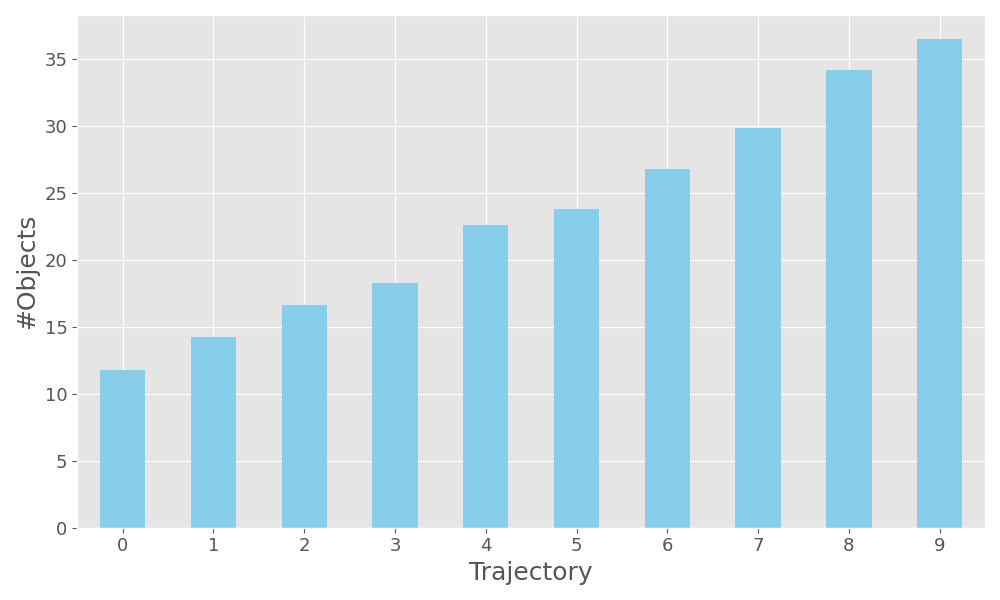
\includegraphics[width=\textwidth]{figures/10_traces/objects.png}
    \caption{Number of objects in every trajectory of $\Ttrain$ averaged among all domains.}
  \end{subfigure}
  \hfill
  \begin{subfigure}[b]{0.48\textwidth}
    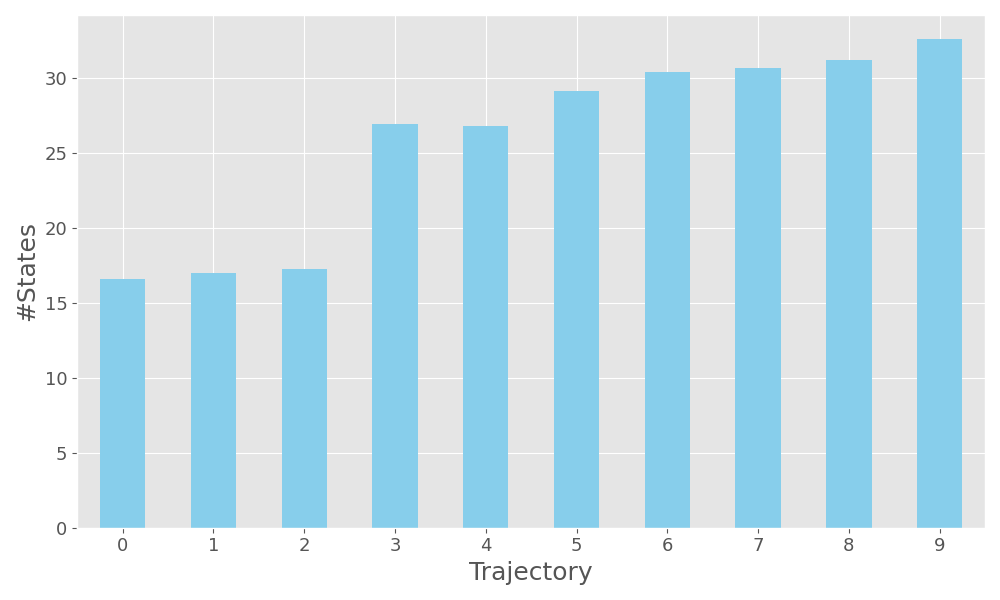
\includegraphics[width=\textwidth]{figures/10_traces/states.png}
    \caption{Number of states in every trajectory of $\Ttrain$ averaged among all domains.}
  \end{subfigure}
  
% \caption{Evaluation metric values for the models learned by \sam, \offlam, \nolam in every benchmark domain. The training set $\Ttrain$ includes $10$ trajectories for every domain.}
\end{figure} 
\vspace{4cm}
\subsection{Detailed Experimental Results}

\begin{table}[h]
\centering
\resizebox{1\columnwidth}{!}{
\begin{tabular}{l|c|c|c|c|c|c|c|c}
% \toprule
\hline
% Domain & Syn. P $\uparrow$ & Syn. R $\uparrow$ & App. P $\uparrow$ & App. R $\uparrow$ & Pred. effs. P $\uparrow$ & Pred. effs. R $\uparrow$ & Solving ratio $\uparrow$ & False plans ratio $\downarrow$ \\
Domain & \multicolumn{2}{c|}{Syntactic} & \multicolumn{2}{c|}{Applicability} & \multicolumn{2}{c|}{Predicted effects} & Solvability \% $\uparrow$ & False plans \% $\downarrow$ \\
 & \makecell[c]{P$\uparrow$} & \makecell[c]{R$\uparrow$} & \makecell[c]{P$\uparrow$} & \makecell[c] {R$\uparrow$} &  \makecell[c]{P$\uparrow$} & \makecell[c] {R$\uparrow$} & & \\
% \midrule
\hline
barman  & 0.95 $^{2}$ & 1.0 $^{1,2,3}$ & 1.0 $^{1,2,3}$ & 0.94 $^{2}$ & 1 $^{1,2,3}$ & 1 $^{1,2,3}$ & 1.0 $^{2}$ & 0 $^{1,2,3}$ \\
blocksworld  & 1.0 $^{2}$ & 1.0 $^{1,2,3}$ & 1.0 $^{1,2,3}$ & 1.0 $^{1,2,3}$ & 1 $^{1,2,3}$ & 1 $^{1,2,3}$ & 1.0 $^{1,2,3}$ & 0 $^{1,2,3}$ \\
childsnack  & 0.97 $^{2}$ & 0.9 $^{1}$ & 1.0 $^{1}$ & 1.0 $^{2}$ & 1 $^{1,2,3}$ & 1 $^{1,2,3}$ & 1.0 $^{1}$ & 0 $^{1}$ \\
depots  & 0.98 $^{2}$ & 1.0 $^{1,2,3}$ & 1.0 $^{1,2,3}$ & 1.0 $^{2}$ & 1 $^{1,2,3}$ & 1 $^{1,2,3}$ & 1.0 $^{1,2,3}$ & 0 $^{1,2,3}$ \\
elevators  & 0.81 $^{2}$ & 1.0 $^{1,2,3}$ & 1.0 $^{1,2,3}$ & 1.0 $^{2}$ & 1 $^{1,2,3}$ & 1 $^{1,2,3}$ & 1.0 $^{2}$ & 0 $^{1,2,3}$ \\
ferry  & 0.93 $^{2}$ & 1.0 $^{1,2,3}$ & 1.0 $^{1,2,3}$ & 1.0 $^{1,2,3}$ & 1 $^{1,2,3}$ & 1 $^{1,2,3}$ & 1.0 $^{1,2,3}$ & 0 $^{1,2,3}$ \\
floortile  & 0.83 $^{2}$ & 1.0 $^{1,2,3}$ & 1.0 $^{1,2,3}$ & 1.0 $^{2}$ & 1 $^{1,2,3}$ & 1 $^{1,2,3}$ & 1.0 $^{2}$ & 0 $^{1,2,3}$ \\
goldminer  & 0.8 $^{2}$ & 0.98 $^{1,2,3}$ & 1.0 $^{1,2,3}$ & 1.0 $^{2}$ & 1 $^{1,2,3}$ & 1 $^{1,2,3}$ & 1.0 $^{1,3}$ & 0 $^{1,3}$ \\
grippers  & 1.0 $^{2}$ & 1.0 $^{1,2,3}$ & 1.0 $^{1,2,3}$ & 1.0 $^{2}$ & 1 $^{1,2,3}$ & 1 $^{1,2,3}$ & 1.0 $^{1,2,3}$ & 0 $^{1,2,3}$ \\
matchingbw  & 0.95 $^{2}$ & 1.0 $^{1,2,3}$ & 1.0 $^{1,2,3}$ & 0.98 $^{1,2,3}$ & 1 $^{1,2,3}$ & 1 $^{1,2,3}$ & 1.0 $^{1,2,3}$ & 0 $^{1,2,3}$ \\
miconic  & 1.0 $^{2}$ & 1.0 $^{1,2,3}$ & 1.0 $^{1,2,3}$ & 1.0 $^{1,2,3}$ & 1 $^{1,2,3}$ & 1 $^{1,2,3}$ & 1.0 $^{1,2,3}$ & 0 $^{1,2,3}$ \\
nomystery  & 0.94 $^{2}$ & 1.0 $^{1,2,3}$ & 1.0 $^{1,2,3}$ & 1.0 $^{2}$ & 1 $^{1,2,3}$ & 1 $^{1,2,3}$ & 1.0 $^{2}$ & 0 $^{1,2,3}$ \\
npuzzle  & 0.88 $^{2}$ & 1.0 $^{1,2,3}$ & 1.0 $^{1,2,3}$ & 1.0 $^{1,2,3}$ & 1 $^{1,2,3}$ & 1 $^{1,2,3}$ & 1.0 $^{1,2,3}$ & 0 $^{1,2,3}$ \\
parking  & 0.89 $^{2}$ & 1.0 $^{1,2,3}$ & 1.0 $^{1,2,3}$ & 1.0 $^{2}$ & 1 $^{1,2,3}$ & 1 $^{1,2,3}$ & 1.0 $^{2}$ & 0 $^{1,2,3}$ \\
rovers  & 0.83 $^{2}$ & 0.93 $^{1,2,3}$ & 1.0 $^{1,2,3}$ & 1.0 $^{2}$ & 1 $^{1,2,3}$ & 1 $^{1,2,3}$ & 1.0 $^{2}$ & 0 $^{1,2,3}$ \\
satellite  & 1.0 $^{2}$ & 1.0 $^{1,2,3}$ & 1.0 $^{1,2,3}$ & 1.0 $^{2}$ & 1 $^{1,2,3}$ & 1 $^{1,2,3}$ & 1.0 $^{1,2,3}$ & 0 $^{1,2,3}$ \\
sokoban  & 0.88 $^{2}$ & 1.0 $^{1,2,3}$ & 1.0 $^{1,2,3}$ & 1.0 $^{1,2,3}$ & 1 $^{1,2,3}$ & 1 $^{1,2,3}$ & 1.0 $^{1,2,3}$ & 0 $^{1,2,3}$ \\
spanner  & 0.93 $^{2}$ & 1.0 $^{1,2,3}$ & 1.0 $^{1,2,3}$ & 1.0 $^{1,2,3}$ & 1 $^{1,2,3}$ & 1 $^{1,2,3}$ & 1.0 $^{1,2,3}$ & 0 $^{1,2,3}$ \\
tpp  & 0.95 $^{2}$ & 1.0 $^{2}$ & 1.0 $^{1,2,3}$ & 1.0 $^{2}$ & 1 $^{1,2,3}$ & 1 $^{1,2,3}$ & 1.0 $^{2}$ & 0 $^{1,2,3}$ \\
transport  & 0.93 $^{2}$ & 1.0 $^{1,2,3}$ & 1.0 $^{1,2,3}$ & 1.0 $^{1,2,3}$ & 1 $^{1,2,3}$ & 1 $^{1,2,3}$ & 1.0 $^{1,2,3}$ & 0 $^{1,2,3}$ \\
% \bottomrule
\hline
\end{tabular}
}
% \caption{Best metric values for every domain obtained among \sam, \offlam, \nolam, respectively denoted by 1,2, and 3; P indicates the precision and R the recall, $\uparrow$ (resp. $\downarrow$) denotes the higher (resp. lower) the better.}
\caption{Best metric values for every domain obtained among \sam, \offlam, \nolam, respectively denoted by 1,2, and 3; P indicates the precision and R the recall, $\uparrow$ (resp. $\downarrow$) denotes the higher (resp. lower) the better. The training set $\Ttrain$ includes $10$ trajectories for every domain.}
\end{table}

\begin{figure}[ht]
% \label{fix:exp-results}
  \centering

  \begin{subfigure}[b]{0.45\textwidth}
    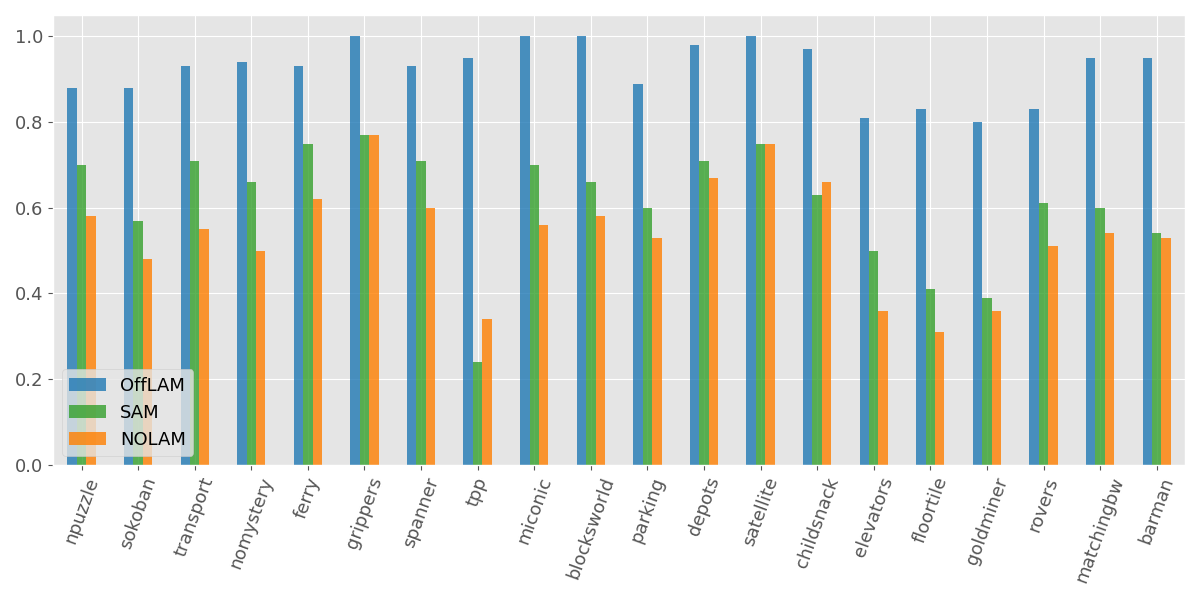
\includegraphics[width=\textwidth]{figures/10_traces/syn_precision.png}
    \caption{Syntactic precision}
  \end{subfigure}
  \hfill
  \begin{subfigure}[b]{0.45\textwidth}
    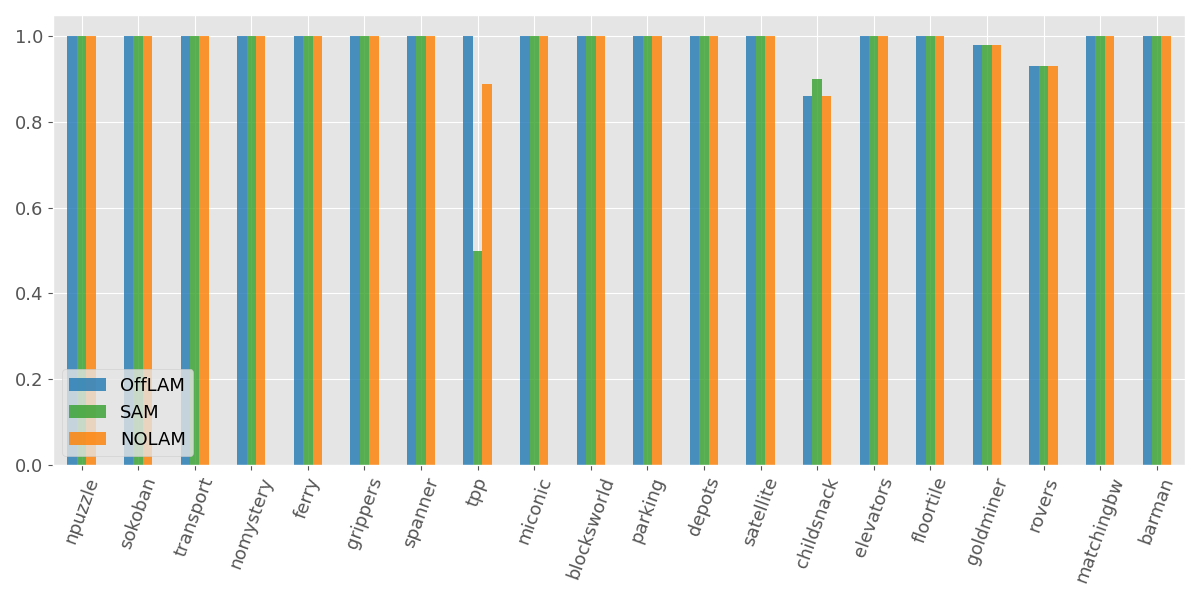
\includegraphics[width=\textwidth]{figures/10_traces/syn_recall.png}
    \caption{Syntactic recall}
  \end{subfigure}

  \vspace{1em}

  \begin{subfigure}[b]{0.45\textwidth}
    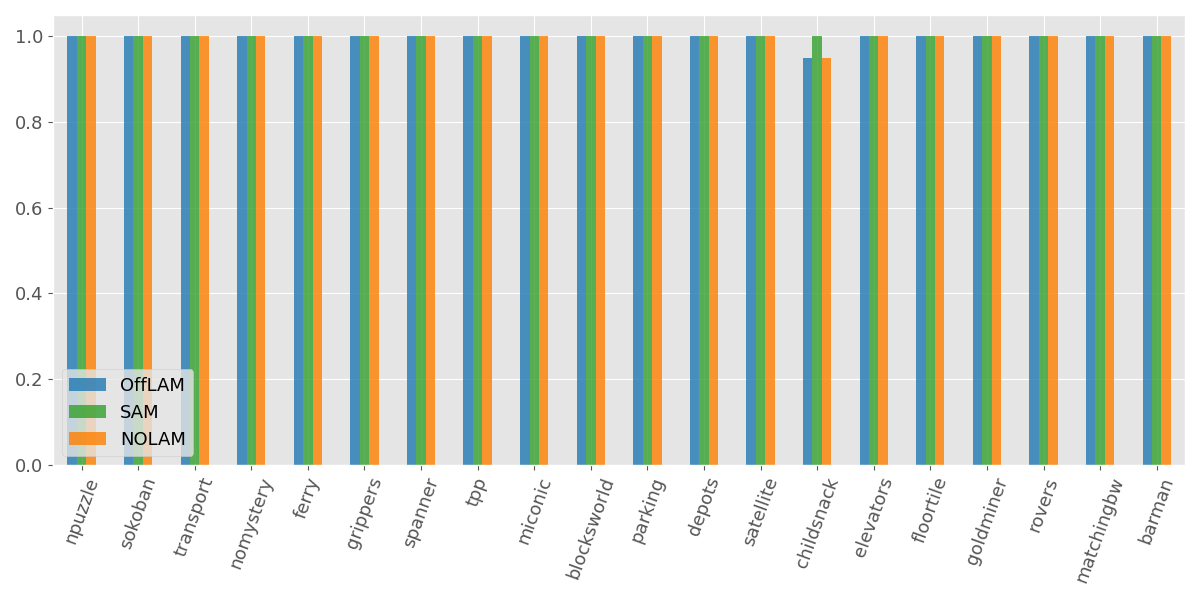
\includegraphics[width=\textwidth]{figures/10_traces/app_precision.png}
    \caption{Applicability precision}
  \end{subfigure}
  \hfill
  \begin{subfigure}[b]{0.45\textwidth}
    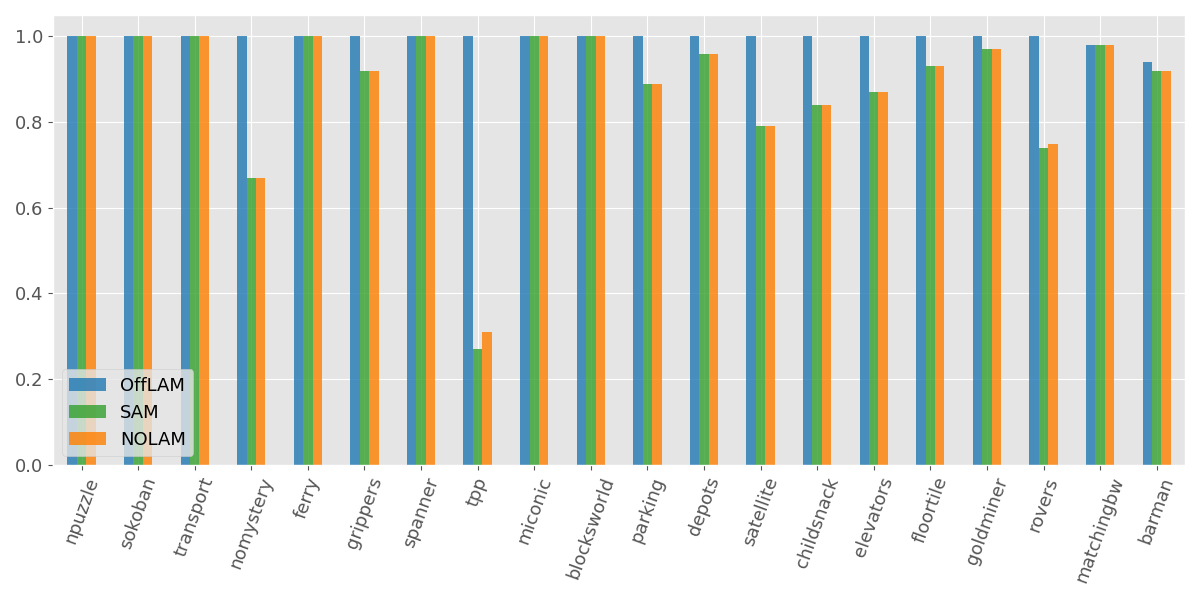
\includegraphics[width=\textwidth]{figures/10_traces/app_recall.png}
    \caption{Applicability recall}
  \end{subfigure}

  \vspace{1em}

  \begin{subfigure}[b]{0.45\textwidth}
    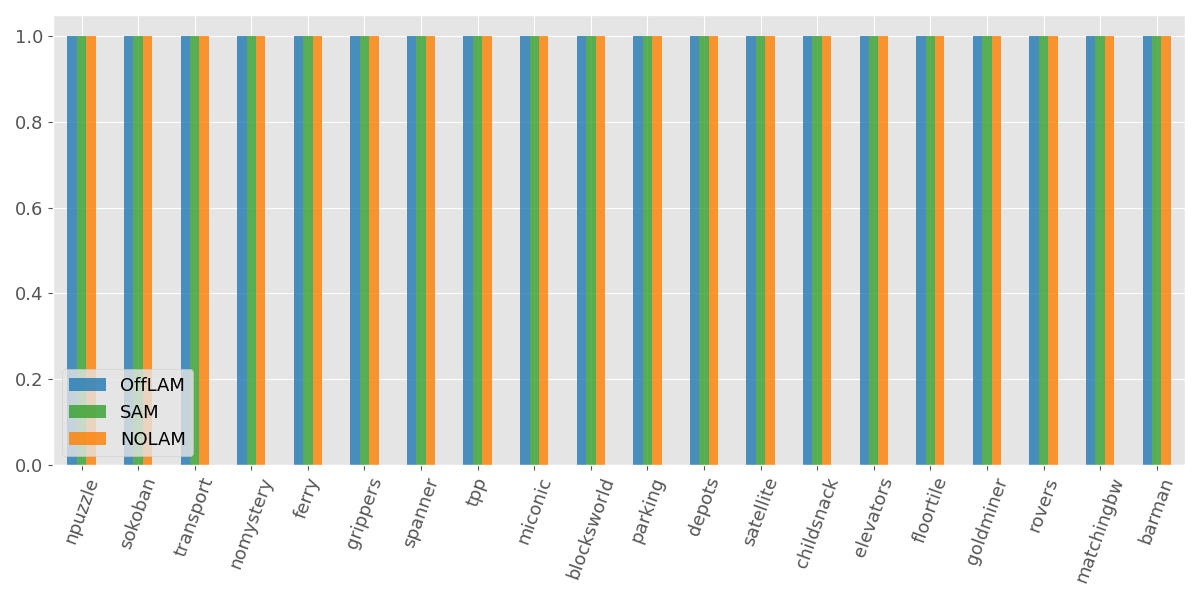
\includegraphics[width=\textwidth]{figures/10_traces/predeffs_precision.png}
    \caption{Predicted effects precision}
  \end{subfigure}
  \hfill
  \begin{subfigure}[b]{0.45\textwidth}
    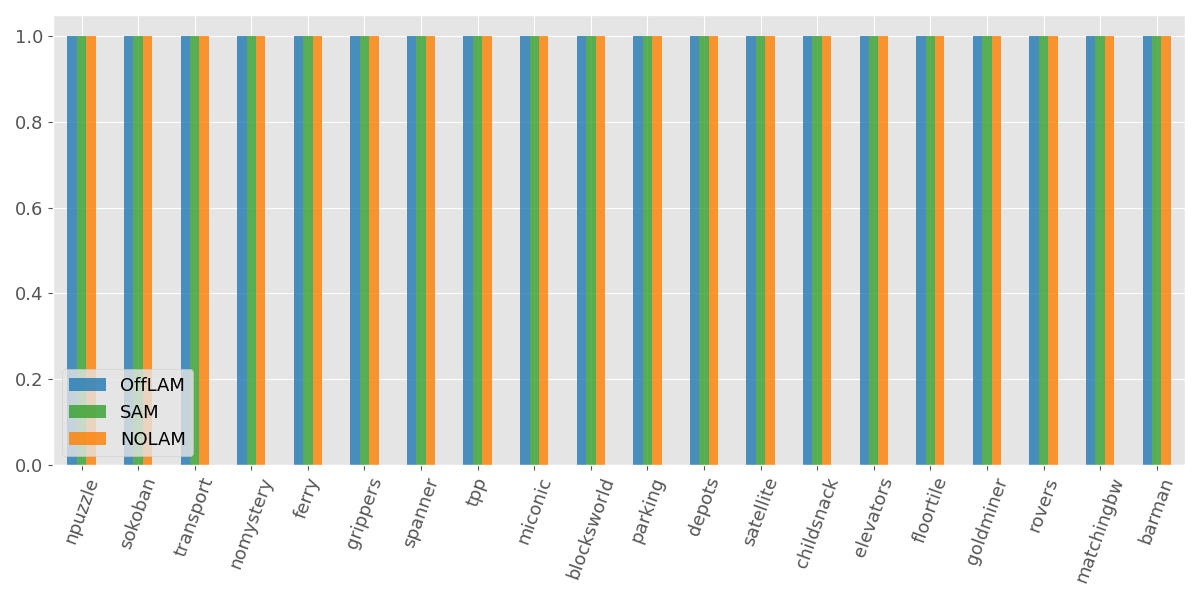
\includegraphics[width=\textwidth]{figures/10_traces/predeffs_recall.png}
    \caption{Predicted effects recall}
  \end{subfigure}

  \vspace{1em}

  \begin{subfigure}[b]{0.45\textwidth}
    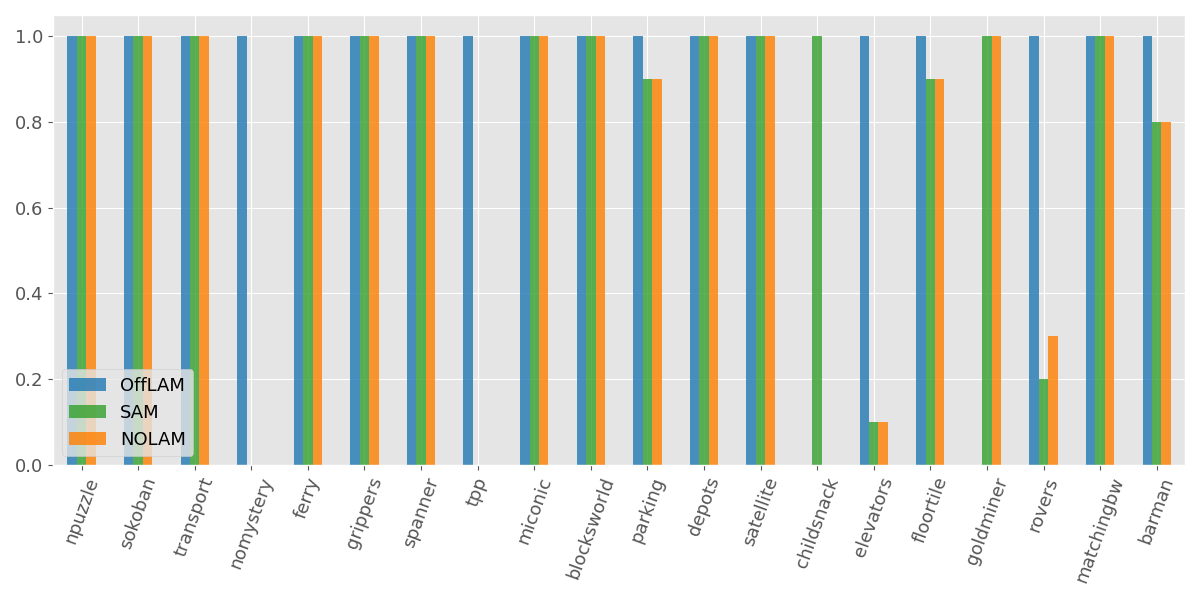
\includegraphics[width=\textwidth]{figures/10_traces/solving.png}
    \caption{Problem solving ratio}
  \end{subfigure}
  \hfill
  \begin{subfigure}[b]{0.45\textwidth}
    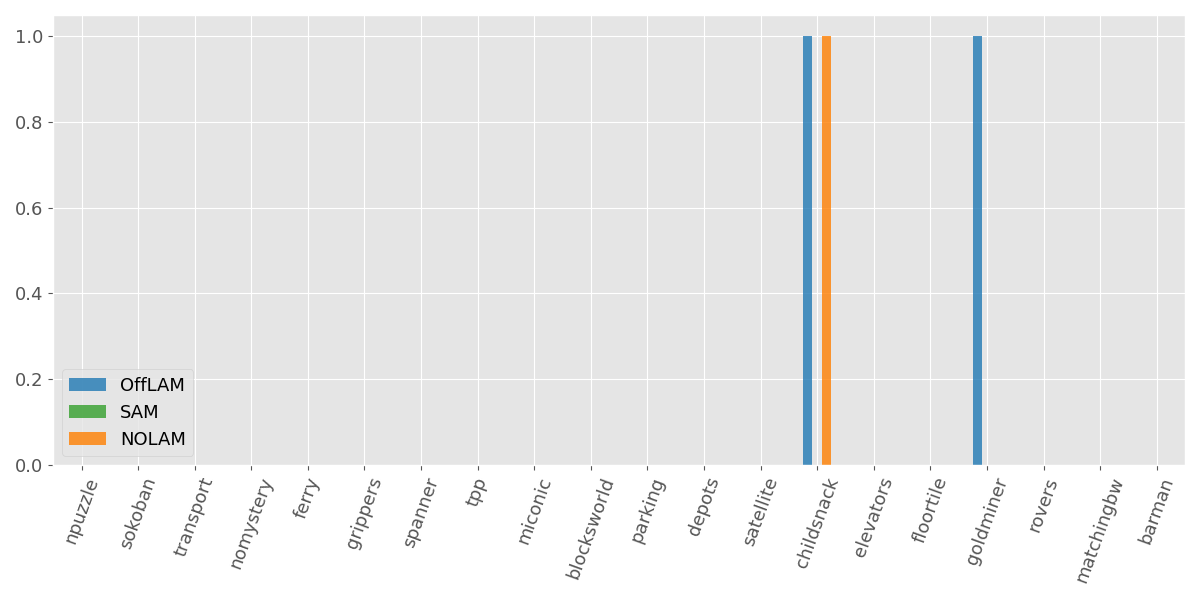
\includegraphics[width=\textwidth]{figures/10_traces/false_plans.png}
    \caption{False plans ratio}
    \label{fig:false-positive-plans}
  \end{subfigure}

  % \caption{Overall caption for the 6 images.}
  % \caption{Evaluation metrics when learning from a training set $\Ttrain$ with $10$ traces for every domain.}
\caption{Evaluation metric values for the models learned by \sam, \offlam, \nolam in every benchmark domain. The training set $\Ttrain$ includes $10$ trajectories for every domain.}
  % \label{fig:exp}
\end{figure} 
% \clearpage


\clearpage
\subsection{Additional Experimental Results}
We also conducted an additional experiments where we generated a training set $\hat{T}_{train}$ with only $2$ trajectories with $10$ states for every domain. To generate this dataset, we produced heuristic plan by considering the $2$ most complex problem settings (in terms of number of objects) adopted for generating the training set with $10$ trajectories for every domain.

\subsection{Training Set $\hat{T}_{train}$ Statistics}
\begin{table}[ht]
\centering
\resizebox{.45\columnwidth}{!}{
\begin{tabular}{l|c|c|c}
% \toprule
\hline
 Domain & \# Objects & \# States & \# Lifted Actions \\
% \midrule
\hline
barman & 33.50 & 9.00 & 10.00 \\
blocksworld & 11.50 & 9.00 & 10.00 \\
childsnack & 38.50 & 9.00 & 10.00 \\
depots & 40.50 & 9.00 & 10.00 \\
elevators & 17.50 & 9.00 & 10.00 \\
ferry & 23.00 & 9.00 & 10.00 \\
floortile & 73.00 & 9.00 & 10.00 \\
goldminer & 33.00 & 9.00 & 10.00 \\
grippers & 27.50 & 9.00 & 10.00 \\
matchingbw & 13.50 & 9.00 & 10.00 \\
miconic & 15.00 & 9.00 & 10.00 \\
nomystery & 23.50 & 9.00 & 10.00 \\
npuzzle & 49.00 & 9.00 & 10.00 \\
parking & 18.00 & 9.00 & 10.00 \\
rovers & 38.50 & 9.00 & 10.00 \\
satellite & 39.50 & 9.00 & 10.00 \\
sokoban & 107.00 & 9.00 & 10.00 \\
spanner & 32.50 & 9.00 & 10.00 \\
tpp & 24.50 & 9.00 & 10.00 \\
transport & 48.50 & 9.00 & 10.00 \\
% \bottomrule
\end{tabular}
}
\caption{Average number of states, objects, and lifted actions in the training set $\hat{T}_{train}$ with $2$ trajectories for every domain.}
% \label{tab:traj-stats}
\end{table}
\vspace{1cm}

\begin{figure}[ht!]
% \label{fix:exp-results}
  \centering

  \begin{subfigure}[b]{0.48\textwidth}
    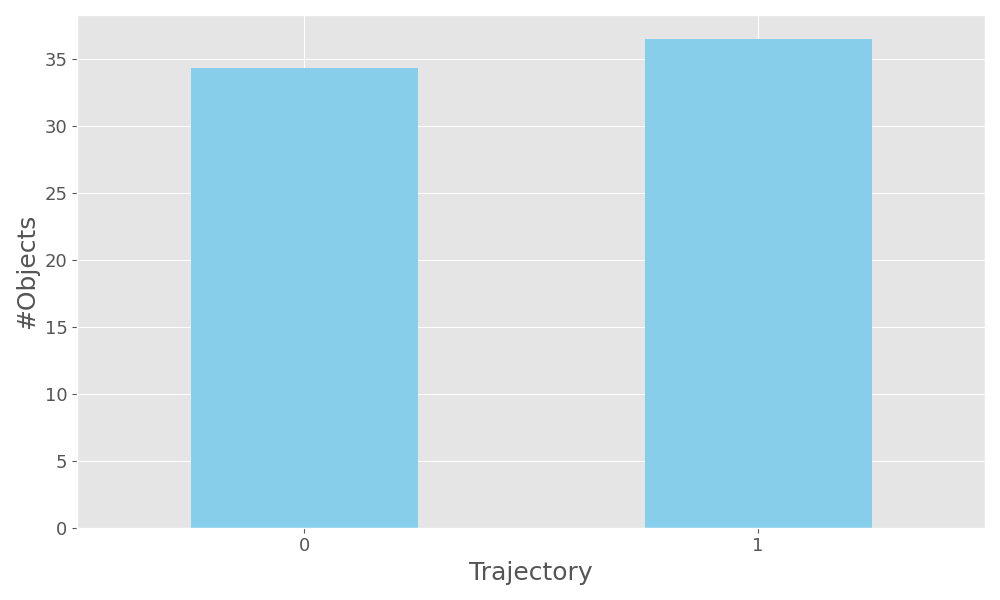
\includegraphics[width=\textwidth]{figures/2_traces/objects.png}
    \caption{Number of objects in every trajectory of $\hat{T}_{train}$ averaged among all domains.}
  \end{subfigure}
  \hfill
  \begin{subfigure}[b]{0.48\textwidth}
    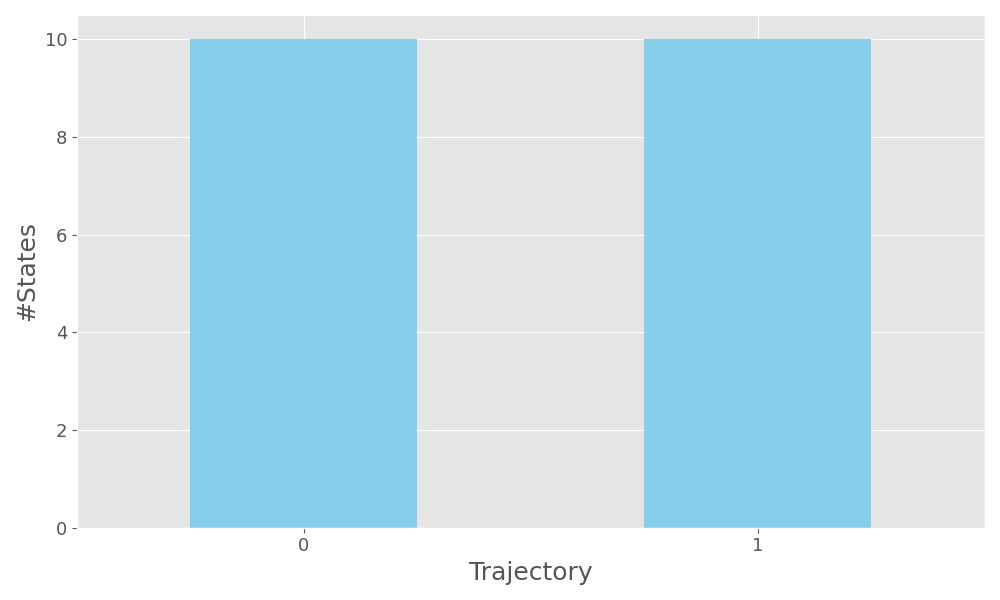
\includegraphics[width=\textwidth]{figures/2_traces/states.png}
    \caption{Number of states in every trajectory of $\hat{T}_{train}$ averaged among all domains.}
  \end{subfigure}
  
% \caption{Evaluation metric values for the models learned by \sam, \offlam, \nolam in every benchmark domain. The training set $\Ttrain$ includes $10$ trajectories for every domain.}
\end{figure} 

\begin{figure}[ht]
  \centering

  \begin{subfigure}[b]{0.45\textwidth}
    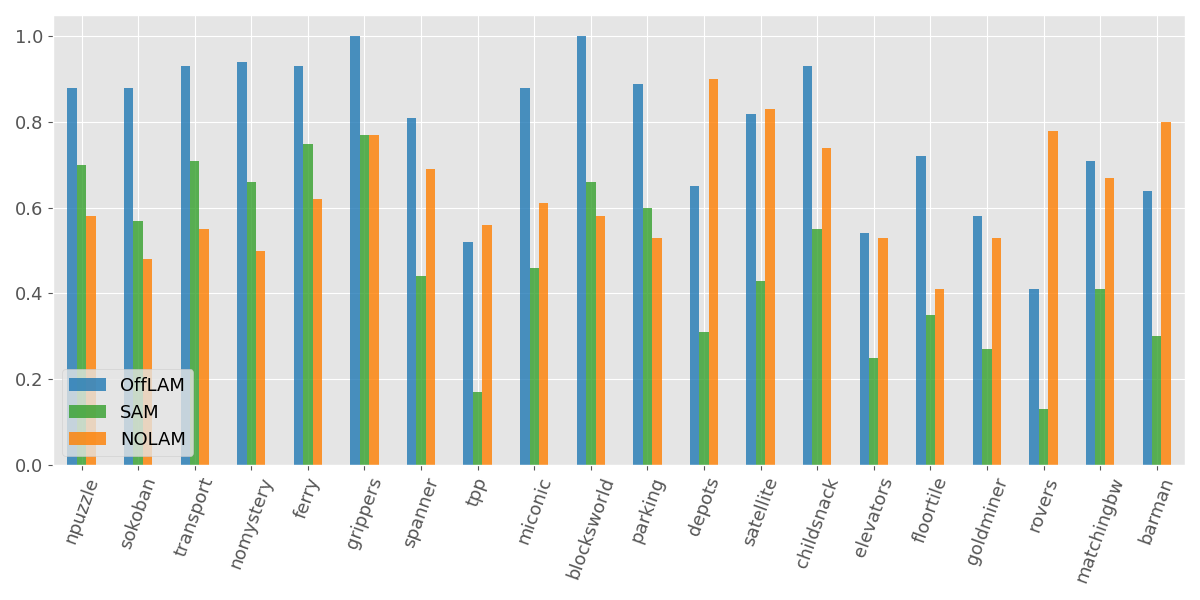
\includegraphics[width=\textwidth]{figures/2_traces/syn_precision.png}
    \caption{Syntactic precision}
  \end{subfigure}
  \hfill
  \begin{subfigure}[b]{0.45\textwidth}
    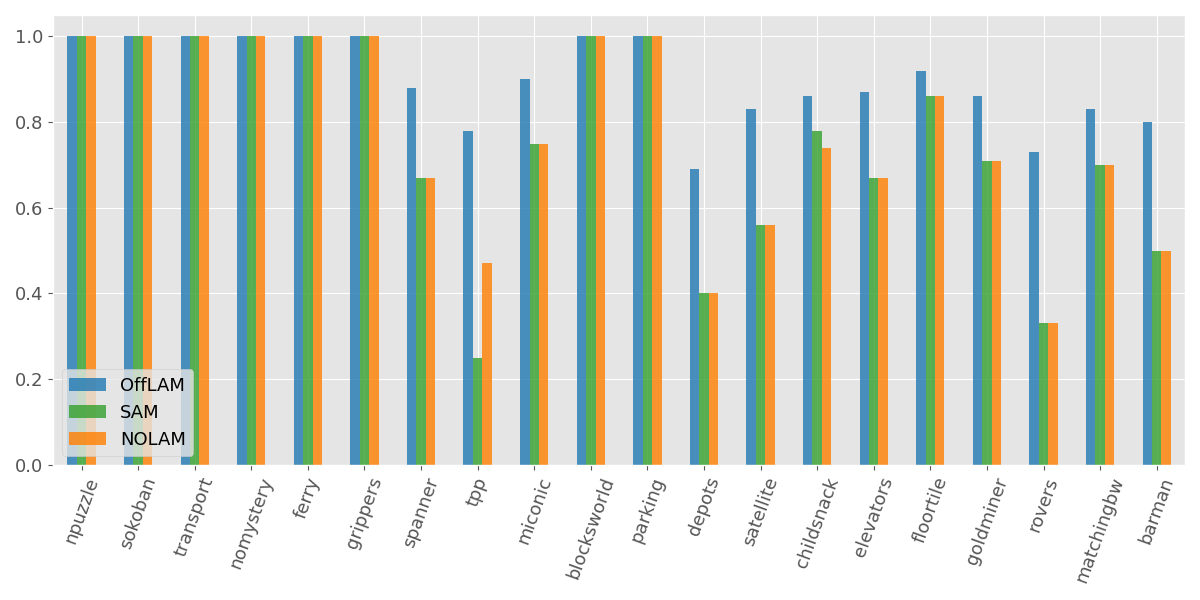
\includegraphics[width=\textwidth]{figures/2_traces/syn_recall.png}
    \caption{Syntactic recall}
  \end{subfigure}

  \vspace{1em}

  \begin{subfigure}[b]{0.45\textwidth}
    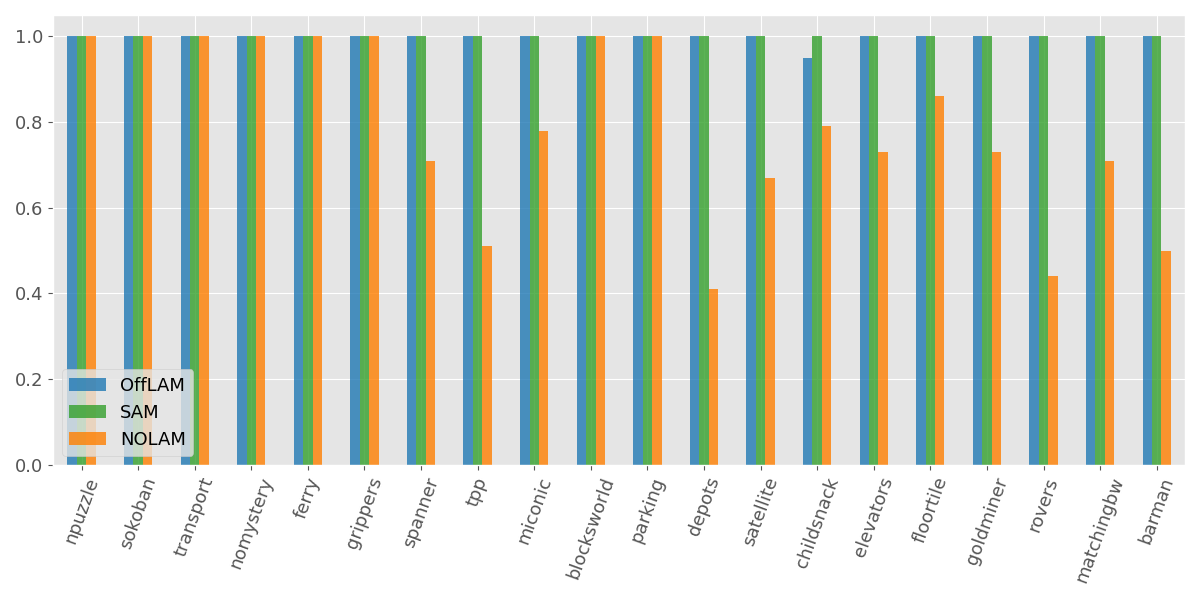
\includegraphics[width=\textwidth]{figures/2_traces/app_precision.png}
    \caption{Applicability precision}
  \end{subfigure}
  \hfill
  \begin{subfigure}[b]{0.45\textwidth}
    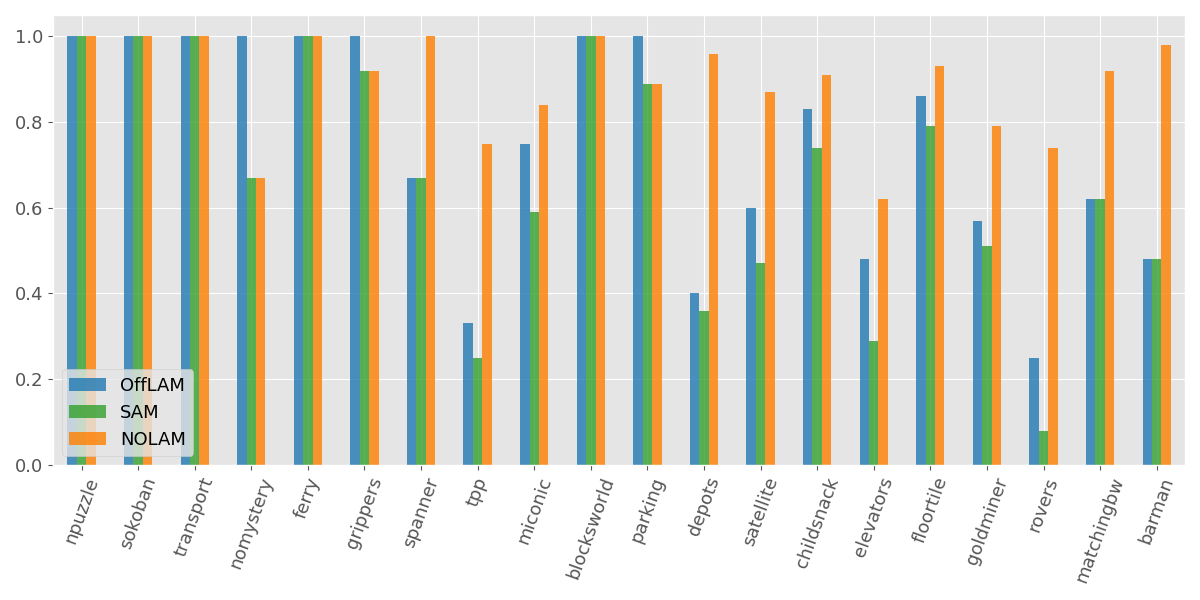
\includegraphics[width=\textwidth]{figures/2_traces/app_recall.png}
    \caption{Applicability recall}
  \end{subfigure}

  \vspace{1em}

  \begin{subfigure}[b]{0.45\textwidth}
    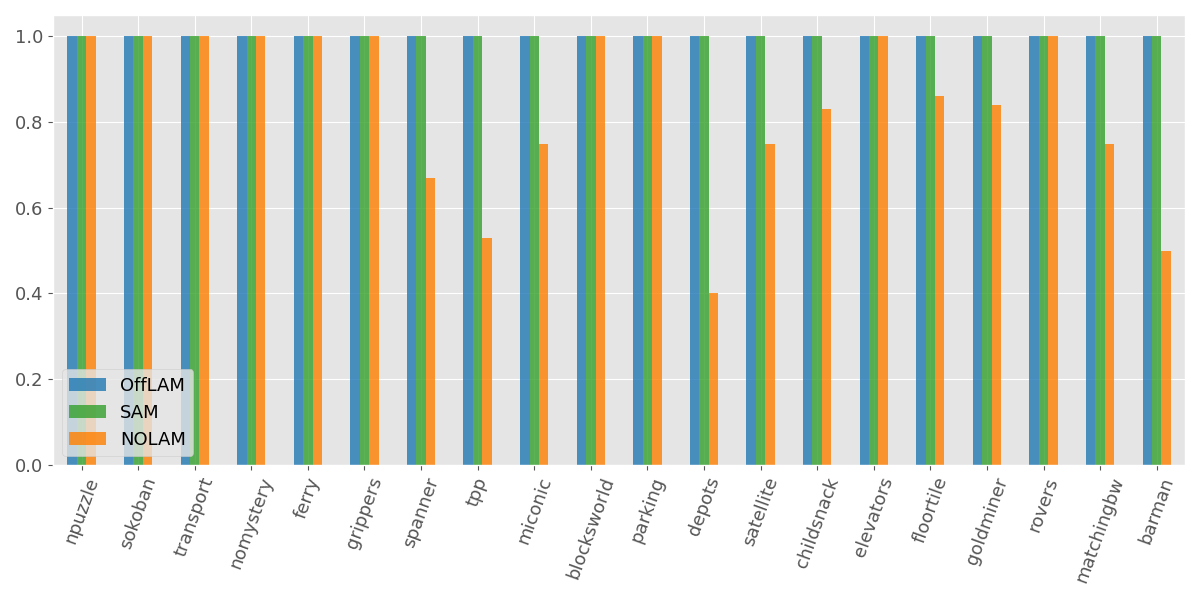
\includegraphics[width=\textwidth]{figures/2_traces/predeffs_precision.png}
    \caption{Predicted effects precision}
  \end{subfigure}
  \hfill
  \begin{subfigure}[b]{0.45\textwidth}
    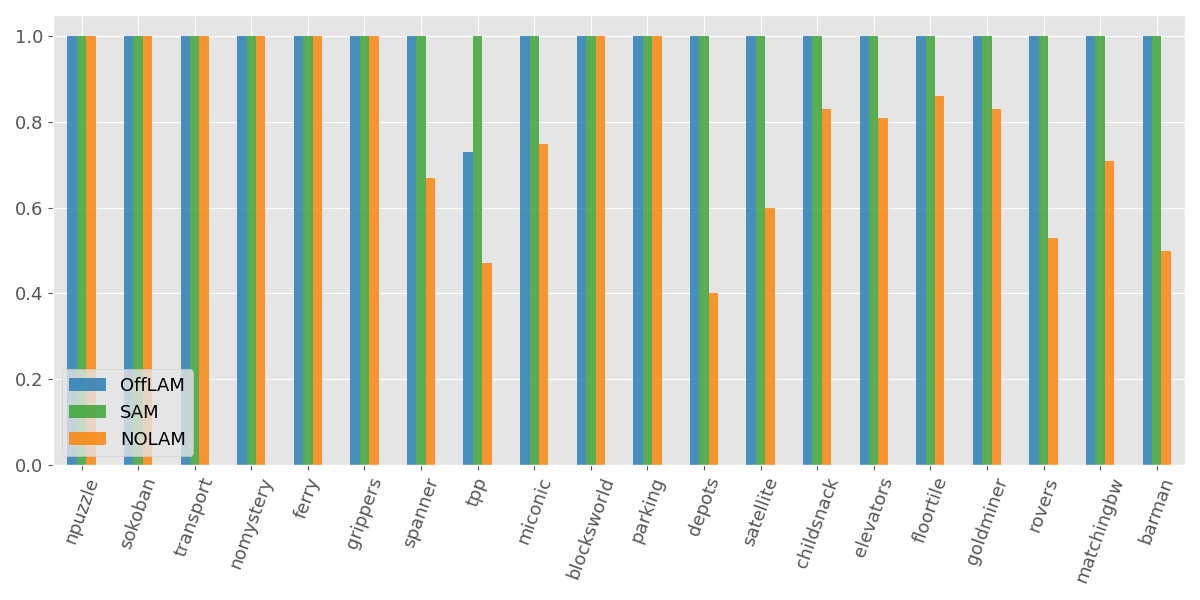
\includegraphics[width=\textwidth]{figures/2_traces/predeffs_recall.png}
    \caption{Predicted effects recall}
  \end{subfigure}

  \vspace{1em}

  \begin{subfigure}[b]{0.45\textwidth}
    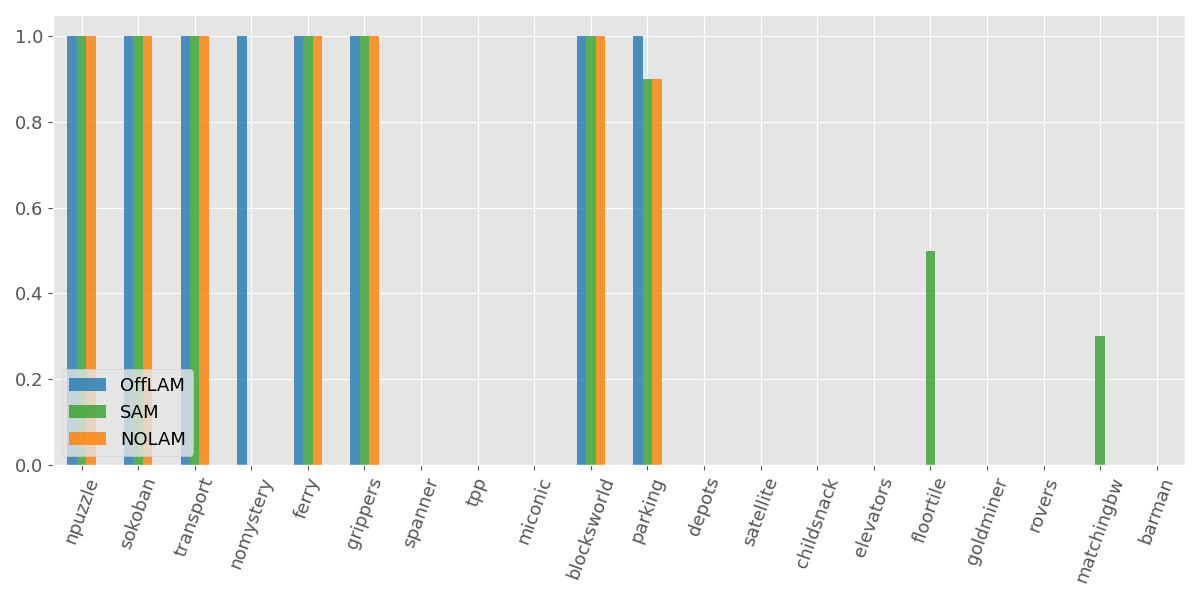
\includegraphics[width=\textwidth]{figures/2_traces/solving.png}
    \caption{Problem solving ratio}
  \end{subfigure}
  \hfill
  \begin{subfigure}[b]{0.45\textwidth}
    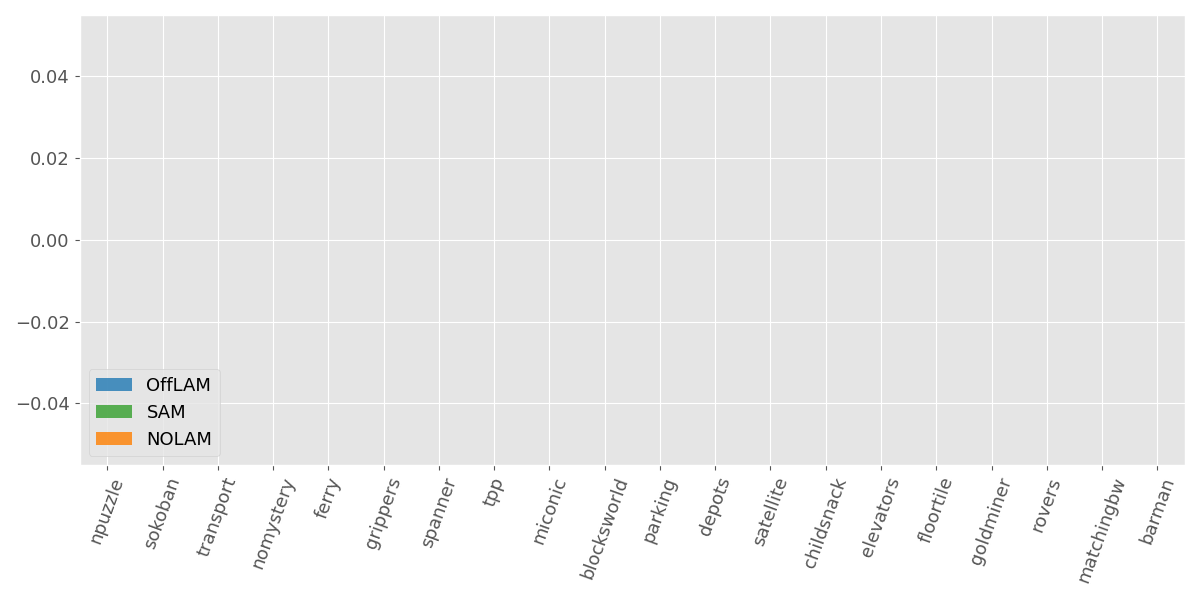
\includegraphics[width=\textwidth]{figures/2_traces/false_plans.png}
    \caption{False plans ratio}
  \end{subfigure}

  % \caption{Overall caption for the 6 images.}
  \caption{Evaluation metrics when learning from a training set $\hat{T}_{train}$ with $2$ traces for every domain.}
\end{figure} 


\begin{table}[h]
\centering
\resizebox{1\columnwidth}{!}{
\begin{tabular}{l|c|c|c|c|c|c|c|c}
% \toprule
\hline
% Domain & Syn. P $\uparrow$ & Syn. R $\uparrow$ & App. P $\uparrow$ & App. R $\uparrow$ & Pred. effs. P $\uparrow$ & Pred. effs. R $\uparrow$ & Solving ratio $\uparrow$ & False plans ratio $\downarrow$ \\
Domain & \multicolumn{2}{c|}{Syntactic} & \multicolumn{2}{c|}{Applicability} & \multicolumn{2}{c|}{Predicted effects} & Solvability \% $\uparrow$ & False plans \% $\downarrow$ \\
 & \makecell[c]{P$\uparrow$} & \makecell[c]{R$\uparrow$} & \makecell[c]{P$\uparrow$} & \makecell[c] {R$\uparrow$} &  \makecell[c]{P$\uparrow$} & \makecell[c] {R$\uparrow$} & & \\
% \midrule
\hline
barman  & 0.8 $^{3}$ & 0.8 $^{2}$ & 1.0 $^{1,2}$ & 0.99 $^{3}$ & 1.0 $^{1,2}$ & 1.0 $^{1,2}$ & 0.0 $^{1,2,3}$ & 0 $^{1,2,3}$ \\
blocksworld  & 1.0 $^{2}$ & 1.0 $^{1,2,3}$ & 1.0 $^{1,2,3}$ & 1.0 $^{1,2,3}$ & 1.0 $^{1,2,3}$ & 1.0 $^{1,2,3}$ & 1.0 $^{1,2,3}$ & 0 $^{1,2,3}$ \\
childsnack  & 0.93 $^{2}$ & 0.86 $^{2}$ & 1.0 $^{1}$ & 0.91 $^{3}$ & 1.0 $^{1,2}$ & 1.0 $^{1,2}$ & 0.0 $^{1,2,3}$ & 0 $^{1,2,3}$ \\
depots & 0.9 $^{3}$ & 0.69 $^{2}$ & 1.0 $^{1,2}$ & 0.96 $^{3}$ & 1.0 $^{1,2}$ & 1.0 $^{1,2}$ & 0.0 $^{1,2,3}$ & 0 $^{1,2,3}$ \\
elevators  & 0.54 $^{2}$ & 0.87 $^{2}$ & 1.0 $^{1,2}$ & 0.63 $^{3}$ & 1.0 $^{1,2,3}$ & 1.0 $^{1,2}$ & 0.0 $^{1,2,3}$ & 0 $^{1,2,3}$ \\
ferry  & 0.93 $^{2}$ & 1.0 $^{1,2,3}$ & 1.0 $^{1,2,3}$ & 1.0 $^{1,2,3}$ & 1.0 $^{1,2,3}$ & 1.0 $^{1,2,3}$ & 1.0 $^{1,2,3}$ & 0 $^{1,2,3}$ \\
floortile & 0.72 $^{2}$ & 0.92 $^{2}$ & 1.0 $^{1,2}$ & 0.93 $^{3}$ & 1.0 $^{1,2}$ & 1.0 $^{1,2}$ & 0.5 $^{1}$ & 0 $^{1,2,3}$ \\
goldminer  & 0.58 $^{2}$ & 0.86 $^{2}$ & 1.0 $^{1,2}$ & 0.78 $^{3}$ & 1.0 $^{1,2}$ & 1.0 $^{1,2}$ & 0.0 $^{1,2,3}$ & 0 $^{1,2,3}$ \\
grippers  & 1.0 $^{2}$ & 1.0 $^{1,2,3}$ & 1.0 $^{1,2,3}$ & 1.0 $^{2}$ & 1.0 $^{1,2,3}$ & 1.0 $^{1,2,3}$ & 1.0 $^{1,2,3}$ & 0 $^{1,2,3}$ \\
matchingbw  & 0.71 $^{2}$ & 0.83 $^{2}$ & 1.0 $^{1,2}$ & 0.92 $^{3}$ & 1.0 $^{1,2}$ & 1.0 $^{1,2}$ & 0.3 $^{1}$ & 0 $^{1,2,3}$ \\
miconic  & 0.88 $^{2}$ & 0.9 $^{2}$ & 1.0 $^{1,2}$ & 0.83 $^{3}$ & 1.0 $^{1,2}$ & 1.0 $^{1,2}$ & 0.0 $^{1,2,3}$ & 0 $^{1,2,3}$ \\
nomystery  & 0.94 $^{2}$ & 1.0 $^{1,2,3}$ & 1.0 $^{1,2,3}$ & 1.0 $^{2}$ & 1.0 $^{1,2,3}$ & 1.0 $^{1,2,3}$ & 1.0 $^{2}$ & 0 $^{1,2,3}$ \\
npuzzle  & 0.88 $^{2}$ & 1.0 $^{1,2,3}$ & 1.0 $^{1,2,3}$ & 1.0 $^{1,2,3}$ & 1.0 $^{1,2,3}$ & 1.0 $^{1,2,3}$ & 1.0 $^{1,2,3}$ & 0 $^{1,2,3}$ \\
parking  & 0.89 $^{2}$ & 1.0 $^{1,2,3}$ & 1.0 $^{1,2,3}$ & 1.0 $^{2}$ & 1.0 $^{1,2,3}$ & 1.0 $^{1,2,3}$ & 1.0 $^{2}$ & 0 $^{1,2,3}$ \\
rovers  & 0.78 $^{3}$ & 0.73 $^{2}$ & 1.0 $^{1,2}$ & 0.73 $^{3}$ & 1.0 $^{1,2,3}$ & 1.0 $^{1,2}$ & 0.0 $^{1,2,3}$ & 0 $^{1,2,3}$ \\
satellite  & 0.83 $^{3}$ & 0.83 $^{2}$ & 1.0 $^{1,2}$ & 0.85 $^{3}$ & 1.0 $^{1,2}$ & 1.0 $^{1,2}$ & 0.0 $^{1,2,3}$ & 0 $^{1,2,3}$ \\
sokoban  & 0.88 $^{2}$ & 1.0 $^{1,2,3}$ & 1.0 $^{1,2,3}$ & 1.0 $^{1,2,3}$ & 1.0 $^{1,2,3}$ & 1.0 $^{1,2,3}$ & 1.0 $^{1,2,3}$ & 0 $^{1,2,3}$ \\
spanner & 0.81 $^{2}$ & 0.88 $^{2}$ & 1.0 $^{1,2}$ & 1.0 $^{3}$ & 1.0 $^{1,2}$ & 1.0 $^{1,2}$ & 0.0 $^{1,2,3}$ & 0 $^{1,2,3}$ \\
tpp  & 0.56 $^{3}$ & 0.78 $^{2}$ & 1.0 $^{1,2}$ & 0.75 $^{3}$ & 1.0 $^{1,2}$ & 1.0 $^{1}$ & 0.0 $^{1,2,3}$ & 0 $^{1,2,3}$ \\
transport  & 0.93 $^{2}$ & 1.0 $^{1,2,3}$ & 1.0 $^{1,2,3}$ & 1.0 $^{1,2,3}$ & 1.0 $^{1,2,3}$ & 1.0 $^{1,2,3}$ & 1.0 $^{1,2,3}$ & 0 $^{1,2,3}$ \\
% \bottomrule
\hline
\end{tabular}
}
% \caption{Best metric values for every domain obtained among \sam, \offlam, \nolam, respectively denoted by 1,2, and 3; P indicates the precision and R the recall, $\uparrow$ (resp. $\downarrow$) denotes the higher (resp. lower) the better.}
\caption{Best metric values for every domain obtained among \sam, \offlam, \nolam, respectively denoted by 1,2, and 3; P indicates the precision and R the recall, $\uparrow$ (resp. $\downarrow$) denotes the higher (resp. lower) the better. The training set $\hat{T}_{train}$ includes $2$ trajectories for every domain.}
\end{table}
}

% RONI: I HOPE YOU ALSO SLEEP SOMETIME ;)

% Yes soon I think.. But you too

% I'm close to converging also, but I want to submit a first version before. Close to it. 
% One thing if we're "talking" to note: I changed the flow a bit in the experimental results so its something like: (1) here's a general way to evaluate model learningn using our metrics, (2) and here's how we impelmented it ( putting here all the details like the planner configuration and all that). I already did this change, just writing so  you're not surprised or annoyed when you read it (after sleeping of course). Hope that's Ok?

% Awesome sure, thanks for saying it (but I think I would not realized it), so I am also converging with the supplementary material (and additional exp with 2 traces), tomorrow morning will polish the code so that we can submit also that

% SOUNDS Great (need to figure out how to anonymize it, but I know there are ways to do it)

% Yes i usually upload the git repo zip by removing the ".git" folder (whichh stores e.g. commit with username etc.)

% Super! TNX

% you too and good night :)


\end{document}

